%*****************************************************A**************************
%********************************** Chapter XXXXXXXX ***************************
%*******************************************************************************

\nomenclature[z-MIP]{MIP}{Minimally Ionising Particle}
\nomenclature[z-MPV]{MPV}{Most Probable Value} 
\nomenclature[z-PID]{PID}{Particle IDentification}
\nomenclature[z-ROI]{ROI}{Region Of Interest}
\nomenclature[z-PoCA]{PoCA}{Point of Closest Approach}

\chapter{Simulations of the 35 ton prototype}  %Title of chapter

\graphicspath{ {35tonSimulation/Figs/PDF/} {35tonSimulation/Figs/Vector/} } %{35tonSimulation/Figs/Raster/}

%********************************** %First Section  *************************************
\section{Determination of interaction times} \label{sec:SimInteractionTimes} %Section - X.1
As outlined at the end of Section~\ref{sec:LArSoft} it is important to know the interaction time of a track when performing calorimetric reconstruction. When performing simulations the simplest interaction time to assign to a reconstructed object is the Monte Carlo truth time of when the particle was created. The creation time can be used as the time taken to travel the relatively modest distances considered in simulations are small when compared to the resolution of the detector (500 ns). When matching a reconstructed object with a GEANT4 particle the particle which contributed the most overall deposited charge to the whole track is chosen. This means that the energy deposited for each hit on the track is broken down into how much each particle contributed to the charge of the individual hit, with the energies summed over all hits. The ability to assign the true interaction times to 3D objects is vital when wanting to benchmark how well other determinations of interaction times perform or to determine the efficiency of the tracking algorithms as described in Section~\ref{sec:SimRecoEffic}. \\

In the 35 ton detector, it was envisioned that there would be at least two ways in which interaction times could be assigned to tracks, one using the external cosmic ray counters and another using reconstructed scintillation light collected by the photon detectors. The cosmic ray counters were used extensively in the 35 ton data, as described in Section~\ref{sec:DataAlgs}, however in simulation the scintillation light was used as this would have been more powerful during continuous running as not all particles would pass through the counters but one wold expect almost all of them to produce reconstructable scintillation light. The flashes of light are reconstructed using a pre-built library which models the expected number of photoelectrons to be measured on each photon detector given the 3D position of the source of the flash. This library takes into account the expected quantum efficiencies of each photon detector. \\

When trying to produce an association metric a sample of 10,000 Anti-Muons with a cosmic-like distribution was used as then there there should only be one long track with which to match one reconstructed flash. A cosmic-like distribution is defined as a set of particles that have a $\cos^{2}$ angular distribution, no minimum or maximum energies and have a uniform $y$ position with flat distrbutions of positions in $x$ and $z$. When this sample was simulated it was clear that the photon detector reconstruction using the pre-built libraries worked well as the reconstructed flash source normally lay very close to the track which caused it. It was found that a calculation of a Point of Closest Approach (PoCA) of the reconstructed track to the flash source gave an effective metric by which the two could be combined. Other metrics such as the distance between the flash source and the track centre, and the perpendicular distance between the flash source and the line joining the start and end of track were investigated but found to provide less reliable metrics. The latter of these metrics is less effective because the reconstructed tracks are rarely straight lines, due to particles scattering as they travel through the LAr and so the perpendicular distance at each hit must be calculated. A comparison of these metrics is shown in Figure~\ref{fig:PDYZDist}. \\

\begin{figure}[h!]
  \centering
  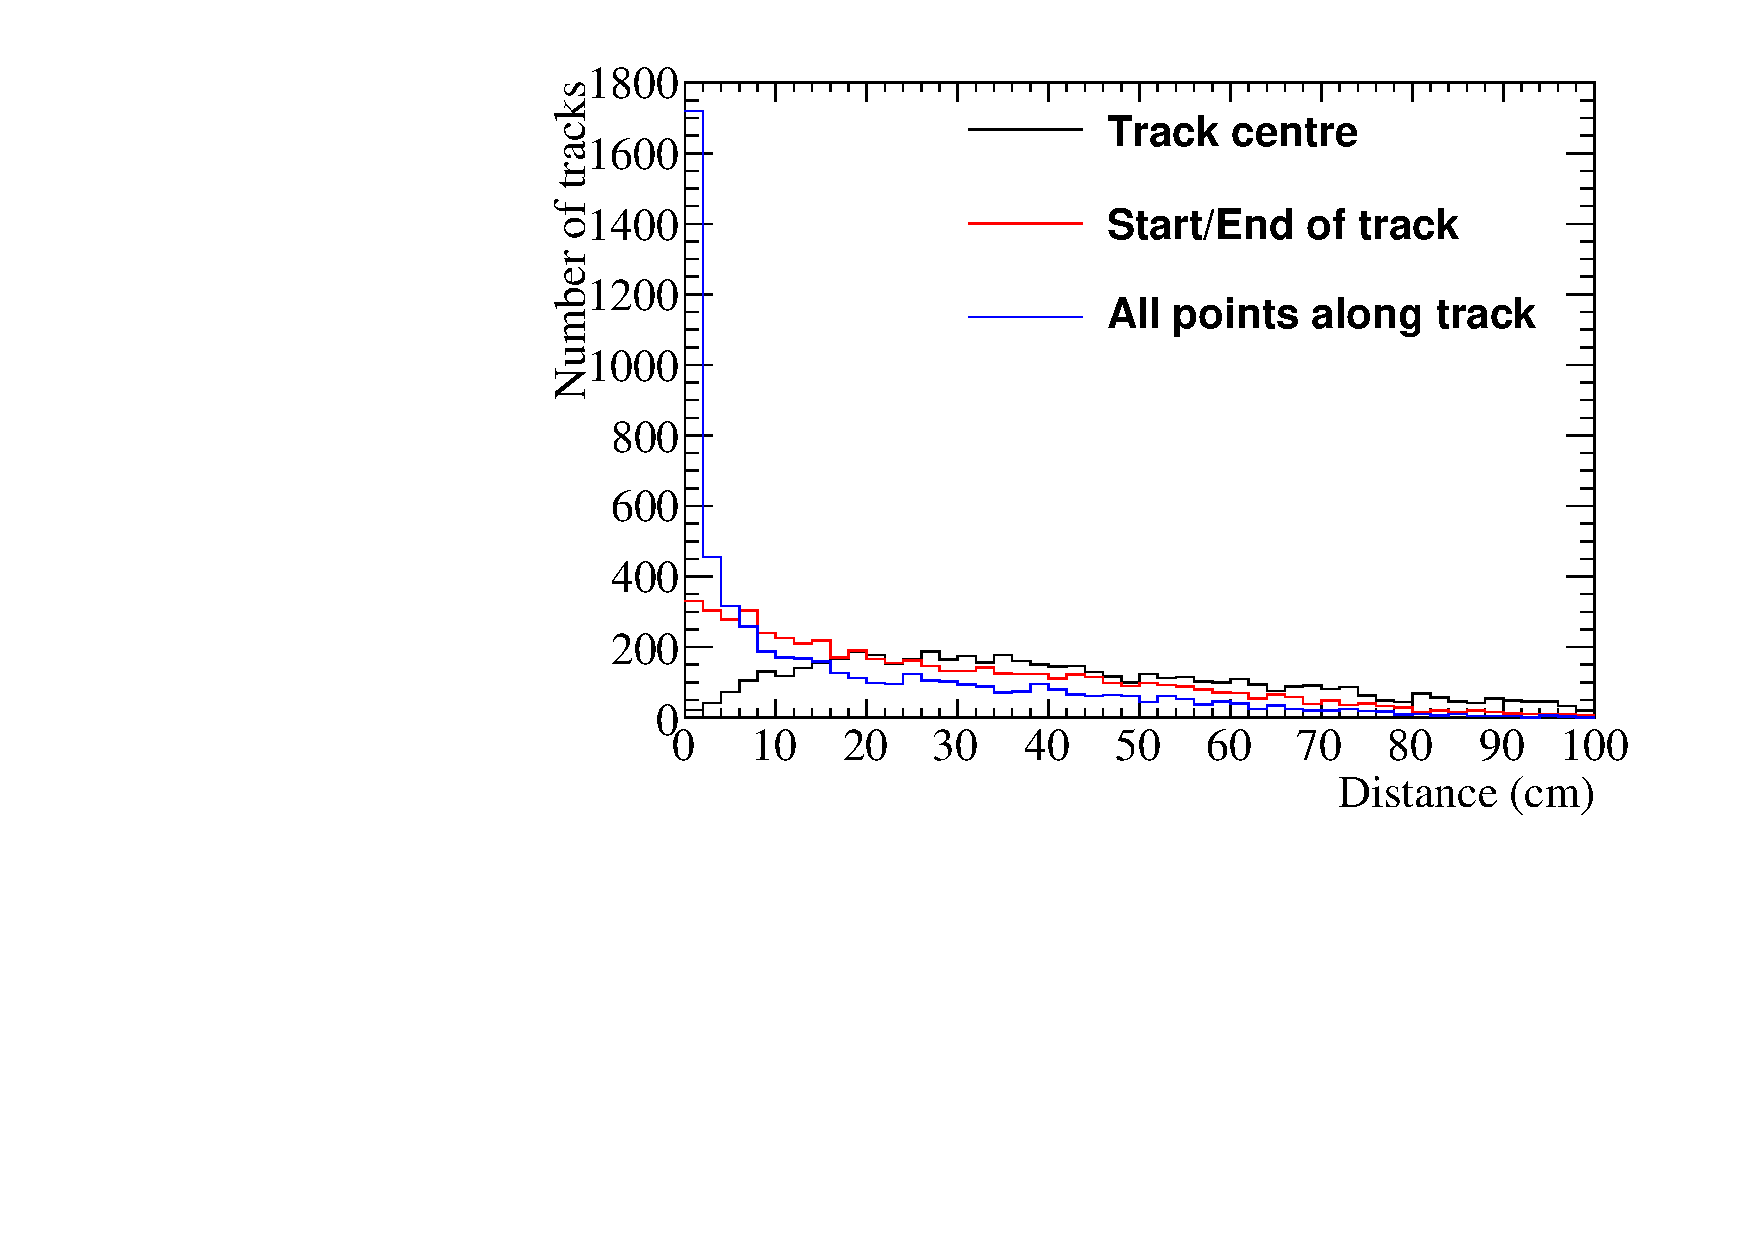
\includegraphics[width=0.5\textwidth]{DiffTrackSeps}
  \caption[Matching tracks and flashes in the 35 ton using positions in the $yz$ plane]
          {A comparison of metrics to match tracks and flashes in the 35 ton detector using the proximity of tracks and flashes in the $yz$ plane.}
  \label{fig:PDYZDist}
\end{figure}

Another metric by which flashes could be assigned to reconstructed tracks is by utilising the relationship between the number of measured photoelectrons and the distance from the APAs at which they were produced. When considering two flashes of scintillation light that are produced at different distances from the APAs, it would be expected that more photoelectrons would be collected when the photons were produced closer to the APAs. This relationship is shown in Figure~\ref{fig:PD_PExPlot} where it can be seen that there is an exponential decay in the number of photoelectrons which are measured with increasing drift distances. Utilising this relationship, means that the distance from the APAs can be predicted from the number of photoelectrons which are measured. This predicted distance from the APA planes can then be compared to the expected $x$ position of a reconstructed track given the difference in flash time and hit times, this is shown in Figure~\ref{fig:PD_PEDiffX}. The difference in these two quantities can then be used as the second metric as it gives an indication of how well the properties of a flash match the reconstructed $x$ position of the track. If the predicted and reconstructed $x$ positions are identical then the track and flash are well matched, this corresponds to the collection of points around the $y=x$ line in Figure~\ref{fig:PD_PEDiffX}. \\

\begin{figure}[h!]
  \centering
  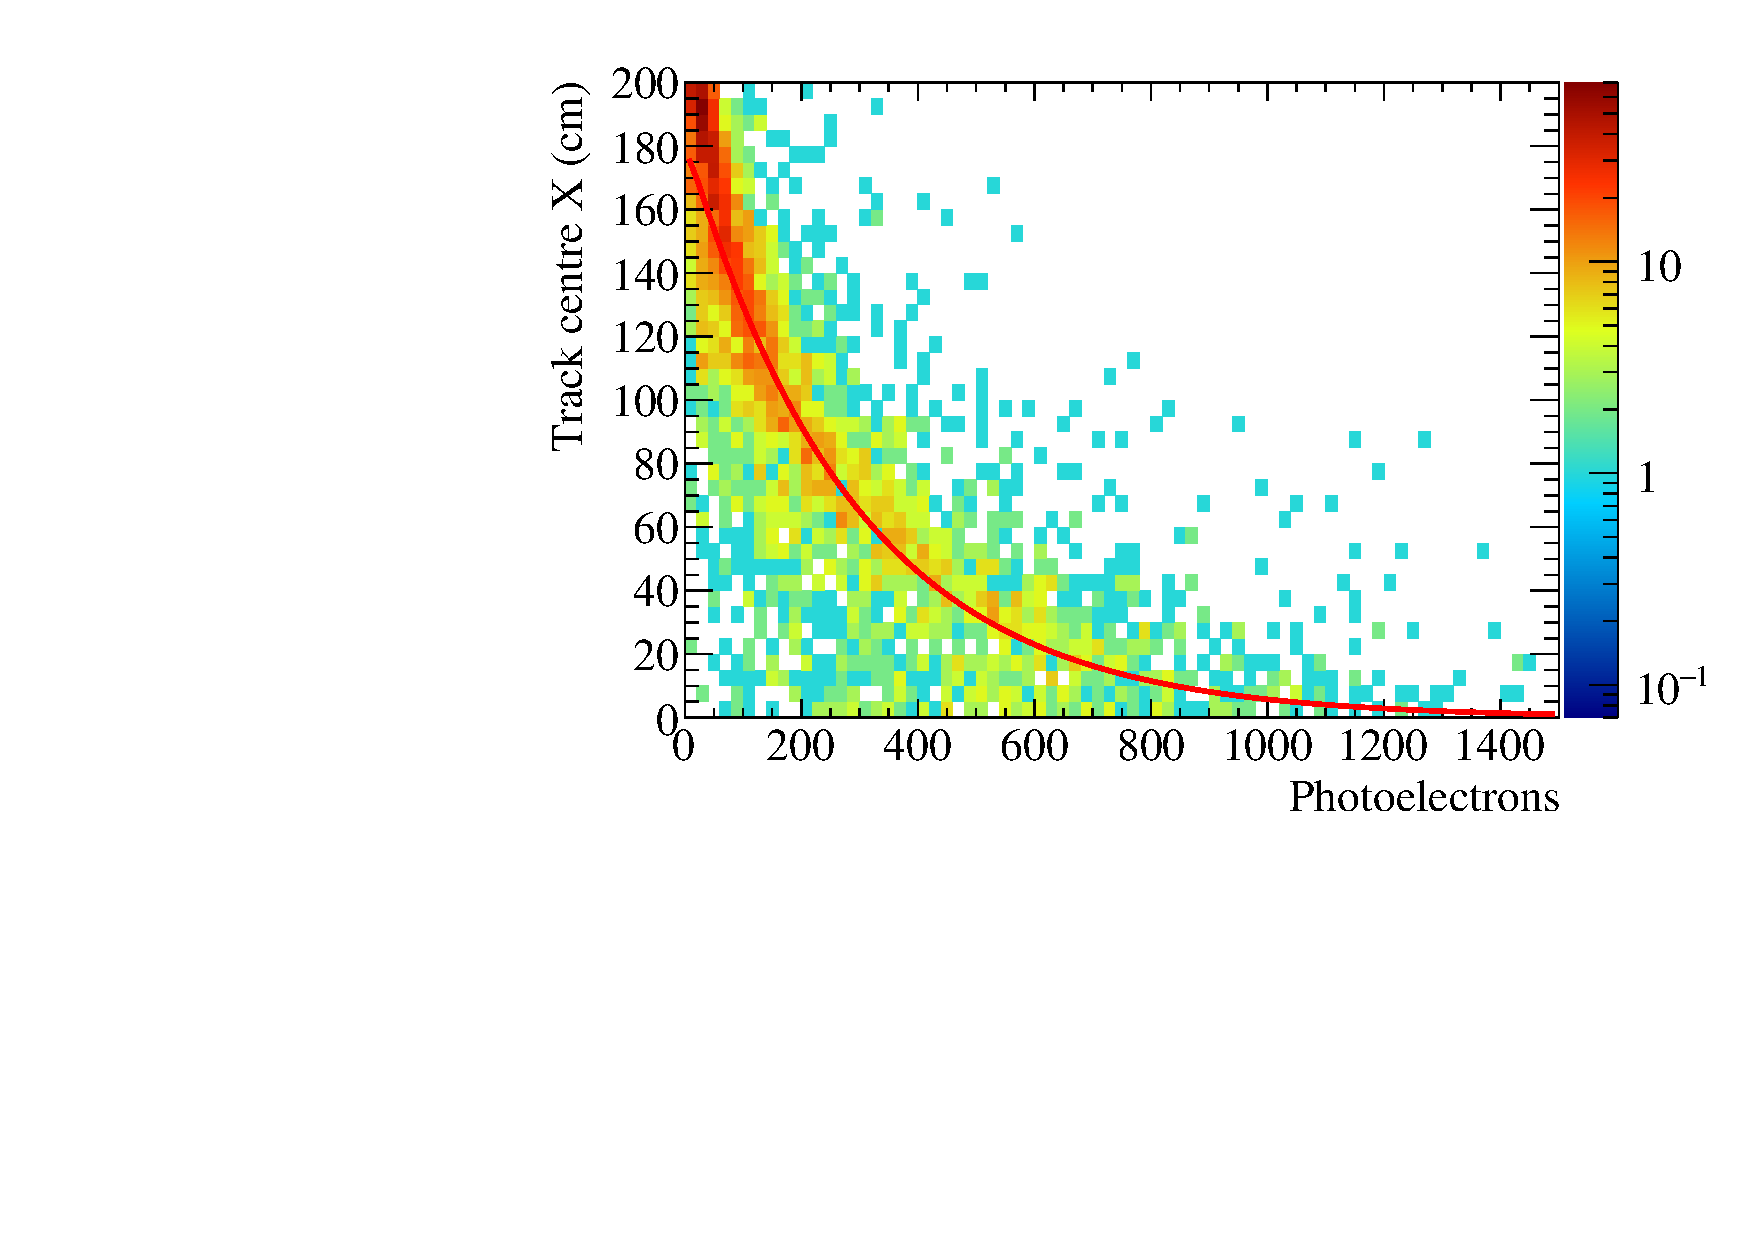
\includegraphics[width=0.6\textwidth]{NumPE_Distance}
  \caption[How the number of photoelectrons measured changes with drift distance]
          {How the number of photoelectrons measured changes with drift distance. The red line corresponds to a parameterisation of the distribution which can be used to predict the $x$ position of a flash given the number of photoelectrons that are collected.}
  \label{fig:PD_PExPlot}
\end{figure}

\begin{figure}[h!]
  \centering
  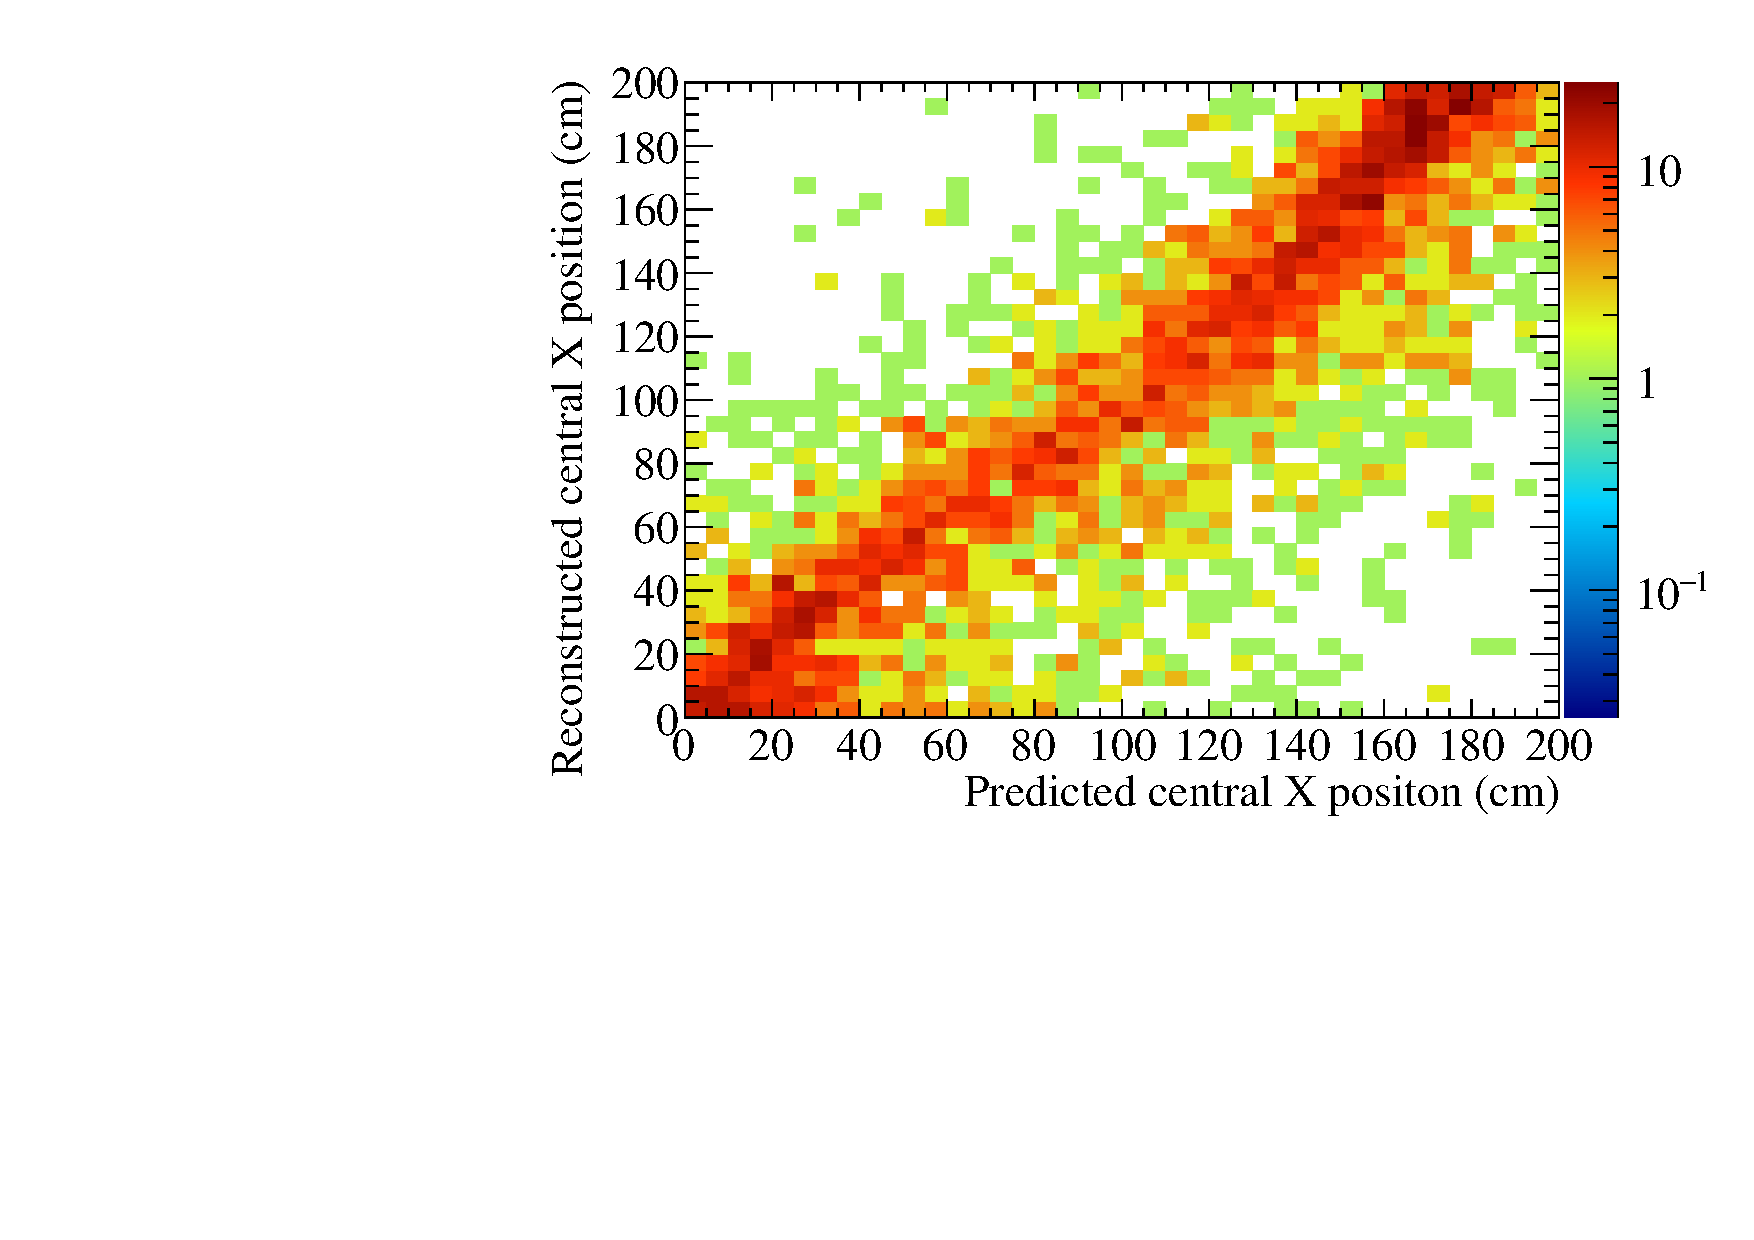
\includegraphics[width=0.6\textwidth]{DiffFlashPredReco}
  \caption[The predited $x$ positions of flashes using the relationship between photoelectron and drift distance]
          {A comparison of the $x$ position predicted using the relationship in Fig~\ref{fig:PD_PExPlot} and the $x$ position predicted by using the difference in flash and hit times.}
  \label{fig:PD_PEDiffX}
\end{figure}

Using these metrics it is possible to attempt to assign reconstructed flashes to reconstructed tracks. Only flashes which are within one drift window of a given track are considered, as flashes outside of this time window cannot have been caused by the reconstructed track. Once flashes are assigned to tracks it is possible to determine how well the matching has performed by comparing the Monte Carlo truth interaction time with the photon detector interaction time. When doing this it is more useful to use a long (16 ms, 32,000 tick) CRY sample as then particles come at random timings as opposed to all at $T$ = 0 in the Anti-Muon sample initially considered. This comparison is shown in Figure~\ref{fig:PD_MCPDDiff}, where there is a clear peak at a time difference of 0 ms in the Monte Carlo truth and photon detector interaction times. When zooming in on this peak it can be seen that there is a systematic offset of 0.6 $\mu$s, this is due to an electronics offset applied in the simulation to the photon detector system. \\

\begin{figure}[h!]
  \centering
  \begin{subfigure}{0.45\textwidth}
    \centering
    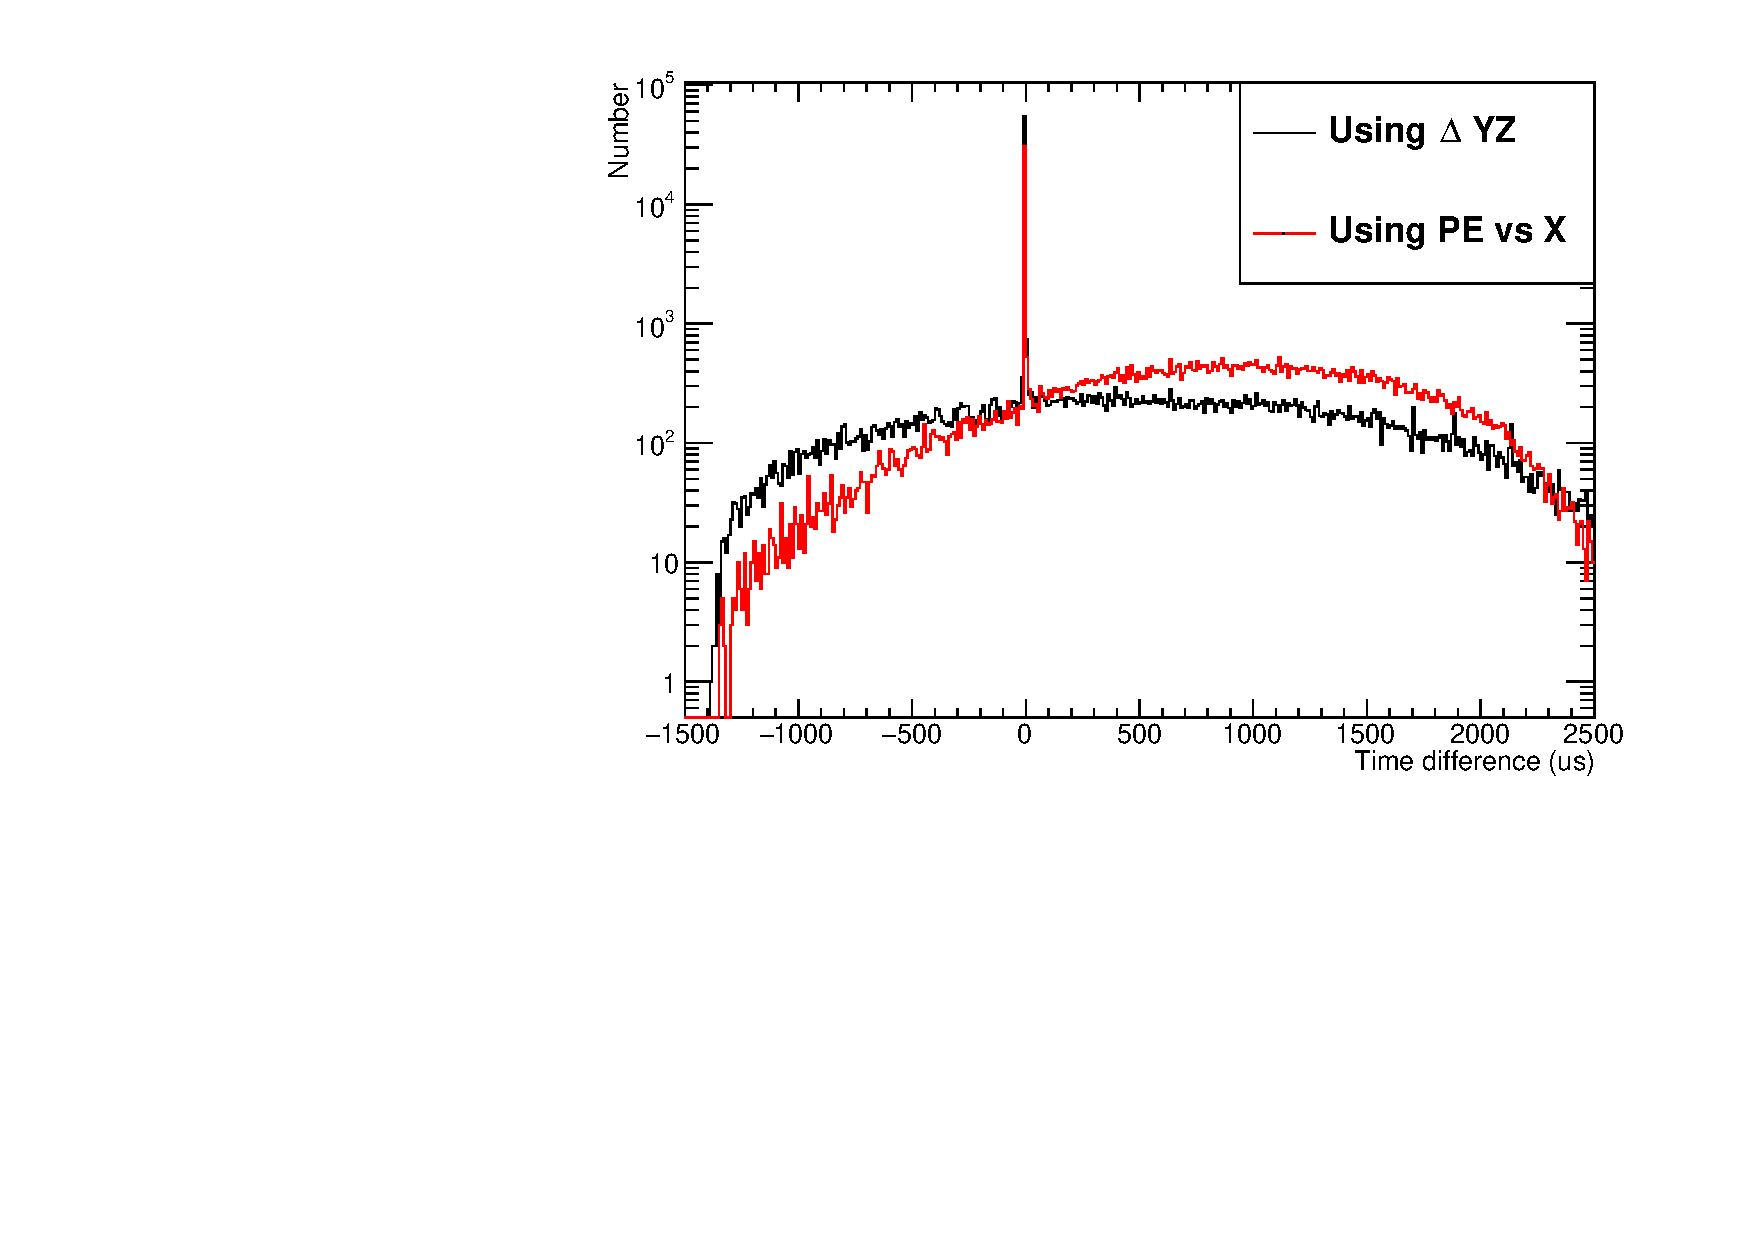
\includegraphics[width=\textwidth]{Pred_Reco_T_Full}
    \caption{The difference in interaction times.}
  \end{subfigure}
  \hspace{0.08\textwidth}
  \begin{subfigure}{0.45\textwidth}
    \centering
    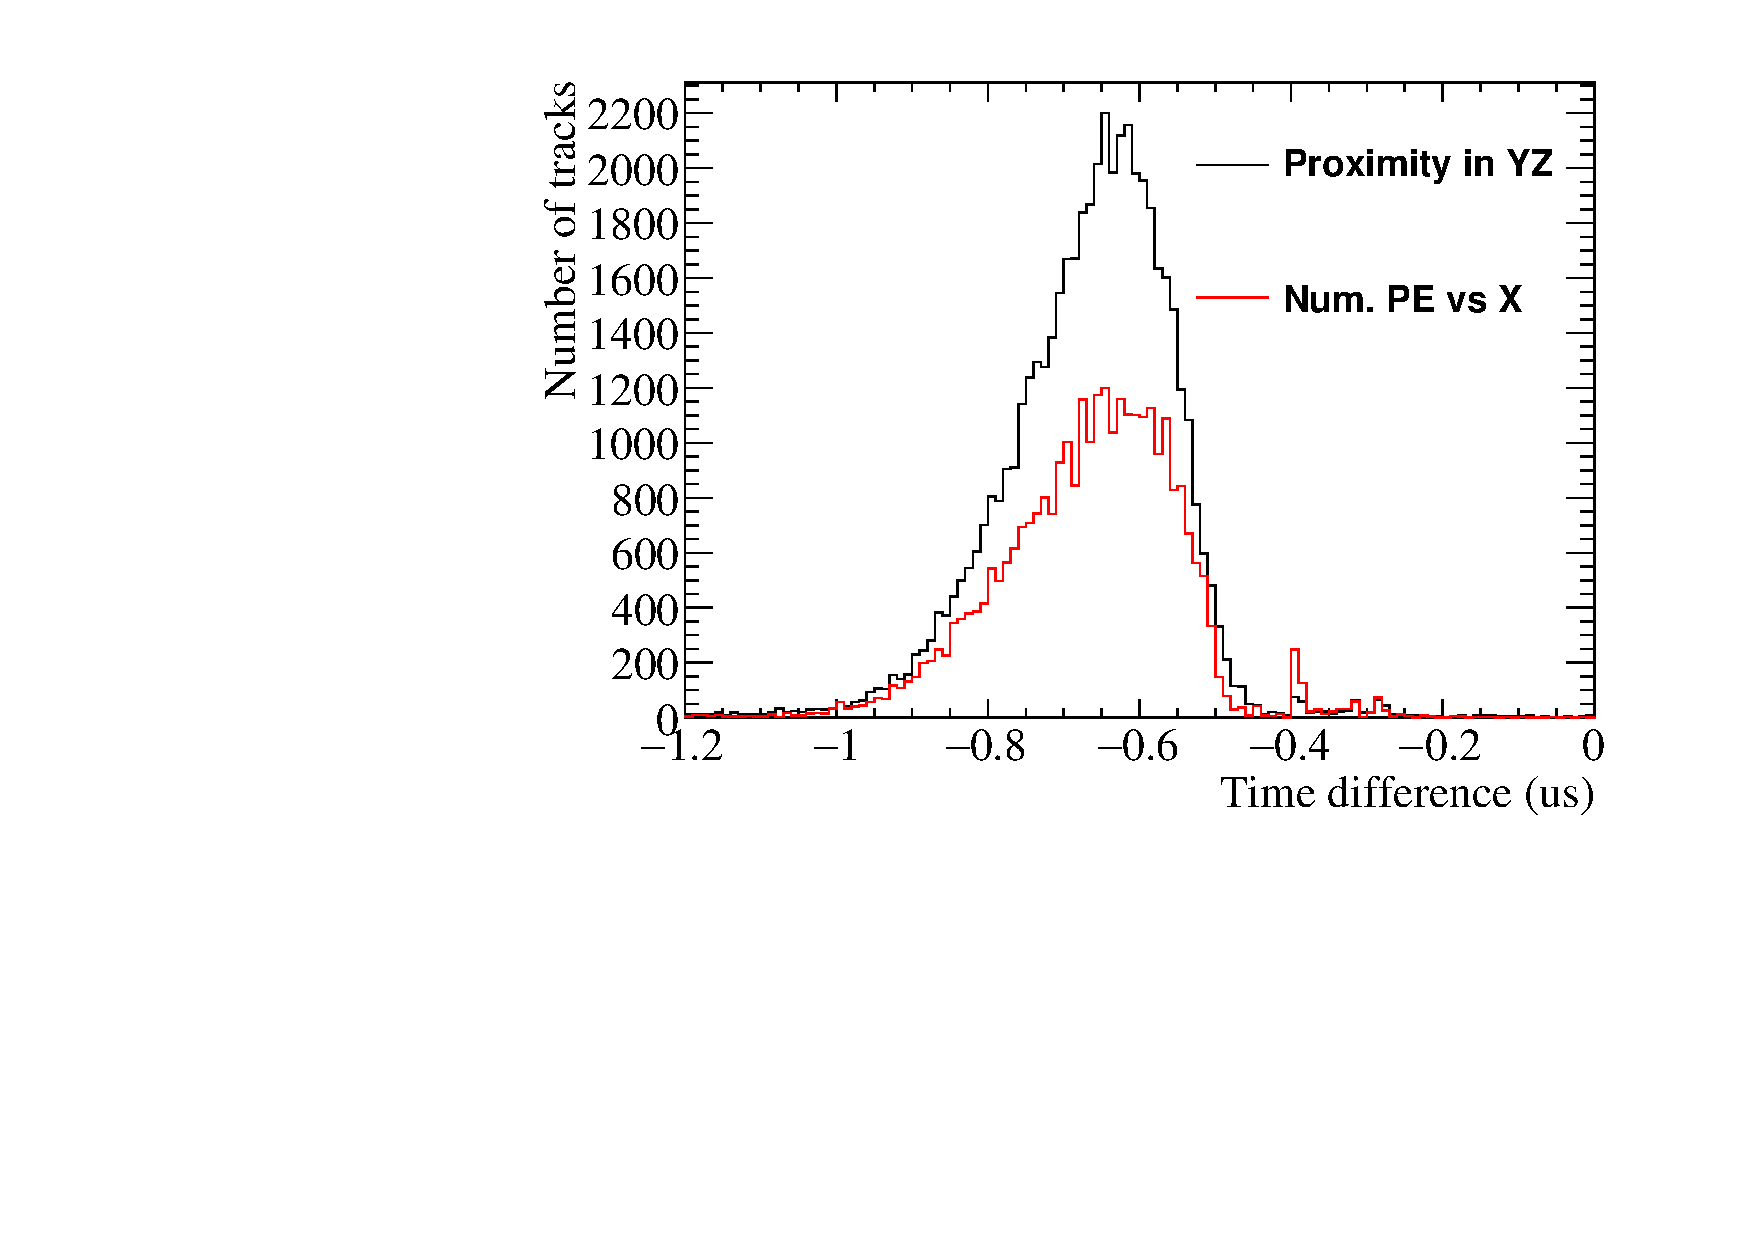
\includegraphics[width=\textwidth]{Pred_Reco_T_Zoom}
    \caption{Zoomed in at low time differences.}
  \end{subfigure}
  \caption[The difference in Monte Carlo interaction times and the predicted interaction times using the photon detectors]
          {The difference in Monte Carlo interaction times and the predicted interaction times using the photon detectors.}
          \label{fig:PD_MCPDDiff}
\end{figure}

From Figure~\ref{fig:PD_MCPDDiff} it can clearly be seen that the metric using the proximity of the flash centre to the track trajectory yields the best matches. This is likely caused by the large spread in the number of photoelectrons collected at fixed drift distances, as shown by Figure~\ref{fig:PD_PExPlot}. The two metrics can be combined to give a prediction for the interaction time, though given the increased sensitivity from the proximity metric this should be given greater weighting. In physics data the metric using the number of collected photoelectrons is particularly sensitive to the absolute light level in the detector as a high residual light level would reduce the proportional change in the number of photoelectrons collected for increasing drift distances. This metric also relies a sample of tracks with known $x$ positions upon which it can be calibrated which may be difficult to obtain. \\

%********************************** % Second Section  *************************************
\section{Calibrating calorimetric constants} \label{sec:MCCalib} %Section - X.2
Having the correct calorimetric responses is vital when trying to calculate $\frac{dE}{dx}$ as the measured change in charge has to be correctly converted to the change in energy. The parameters which need to be tuned in order to ensure that this is done correctly are the $Recomb_A$ and $Recomb_B$ of Equations~\ref{eq:Birks_A}, ~\ref{eq:Birks_B}, ~\ref{eq:ModBox} and ~\ref{eq:ModBox_B},. These parameters have to be tuned in such a way as to make a known particle energy deposition have the correct $\frac{dE}{dx}$, the easiest deposition to tune against is the Minimally Ionising Particle (MIP) peak which in LAr should have a value of 1.8 MeV cm$^{-3}$. To do this the sample of 10,000 Anti-Muons made to calibrate the photon detector track/flash assignment will be used as many of these particles will be MIPs. \\

To select the MIPs in the sample only tracks caused by through-going muons are used. The $\frac{dE}{dx}$ value for all hits in all tracks is then calculated, with the different planes separated out as each one will have its own normalisation factor. A Gaussian distribution is then fitted around the peaks for each of the planes to discern the Most Probable Value (MPV) of $\frac{dE}{dx}$ for that plane. If the MPVs are not equal to 1.8 MeV cm$^{-3}$ then the normalisation factors are scaled through a process of trial and error until the correct MPVs are measured. An example of the tuning being applied is shown in Figure~\ref{fig:CaloTune}. Tuning of the calorimetric constants is required whenever the electronics gains or signal shaping functions are changed.

\begin{figure}[h!]
  \centering
  \begin{subfigure}{0.45\textwidth}
    \centering
    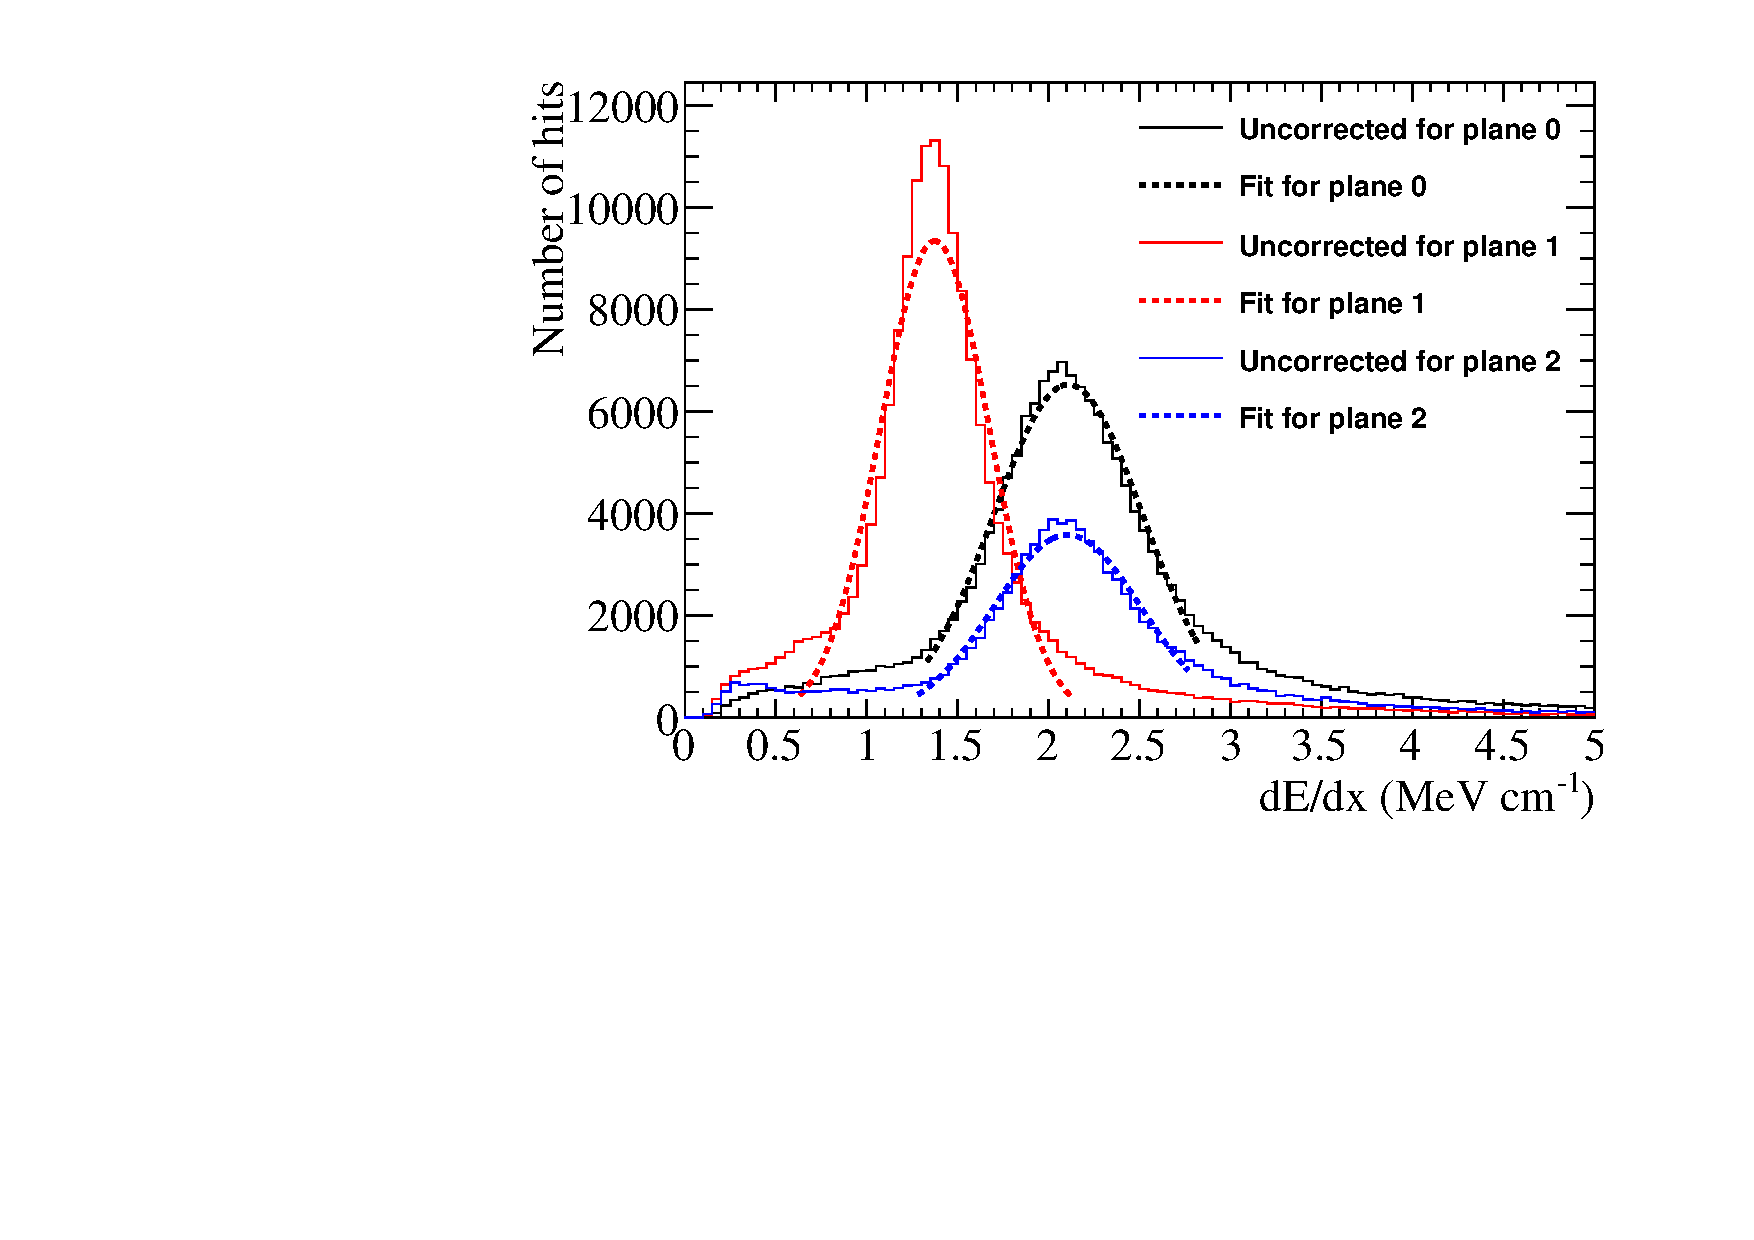
\includegraphics[width=\textwidth]{UnCorrectedCanvas}
    \caption{Before a normalisation correction is applied.}
    \label{fig:CaloTune_Before}
  \end{subfigure}
  \hspace{0.08\textwidth}
  \begin{subfigure}{0.45\textwidth}
    \centering
    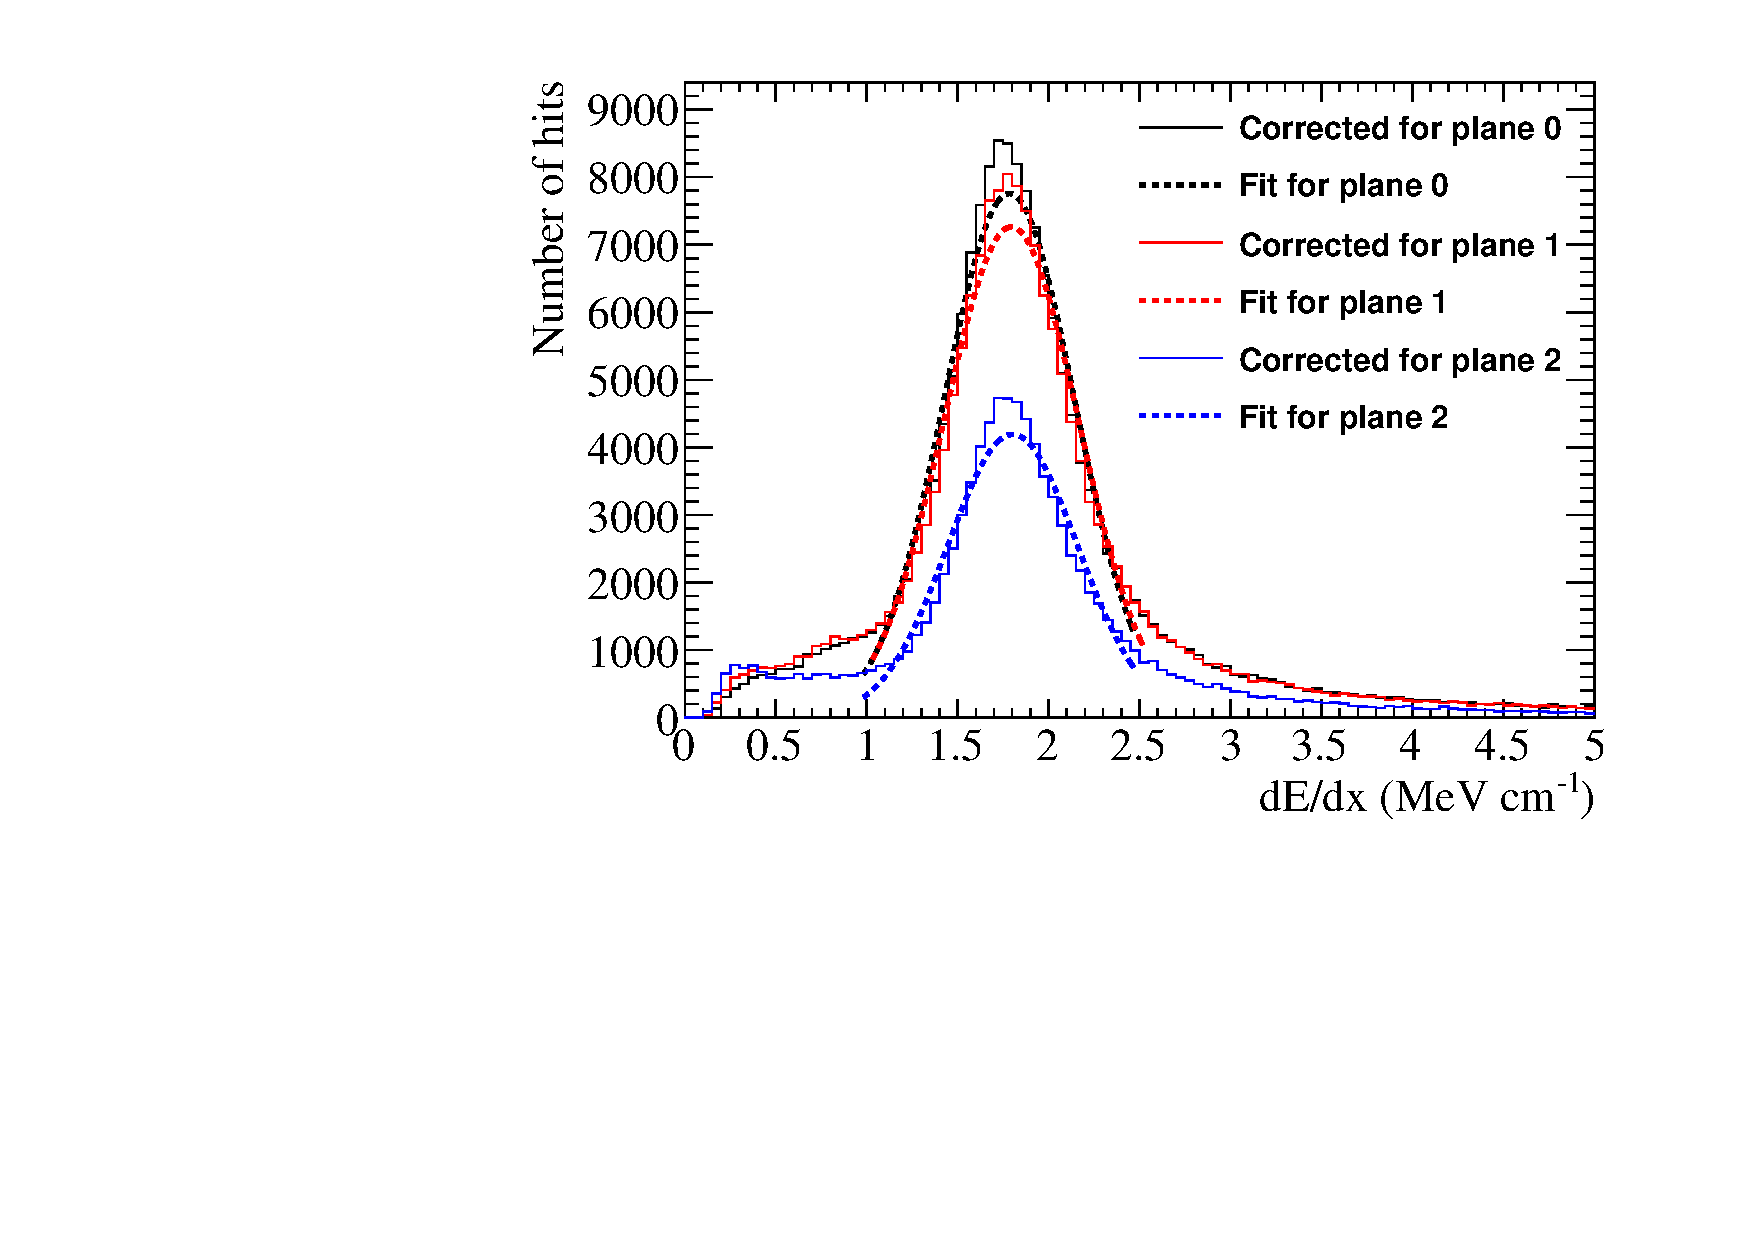
\includegraphics[width=\textwidth]{CorrectedCanvas}
    \caption{After a normalisation correction is applied.}
    \label{fig:CaloTune_After}
  \end{subfigure}
  \caption[The tuning of the calorimetric constants in the 35 ton]
          {How the $\frac{dE}{dx}$ MPVs change for each plane when a change is made to the electronics gains in the 35 ton. Figure~\ref{fig:CaloTune_Before} shows the MPVs before the constants are corrected, whilst Figure~\ref{fig:CaloTune_After} shows the MPVs after the constants are retuned.}
          \label{fig:CaloTune}
\end{figure}
        
%********************************** % Third Section  *************************************
\section{Discerning reconstruction efficiencies} \label{sec:SimRecoEffic} %Section - X.3
Knowledge of the strengths and weaknesses of different tracking algorithms is vital when using them for physics analyses, to this end it is useful to develop a metric by which they can be compared. In order to do this a series of conditions have to be applied to the reconstructed tracks from a large set of simulated particles which are reconstructed using different tracking algorithms. It is interesting to observe what the effect of event complexity has on the reconstruction algorithms and so efficiencies will be calculated for both the Anti-Muon and CRY samples used in Section~\ref{sec:SimInteractionTimes}. \\

The criteria upon which to determine whether a particle is well reconstructed has to be carefully chosen as every definition will have limitations. For example, consider a particle that travels 100 cm in the active volume of the detector but is reconstructed as 2 separate tracks (tracks 1 and 2), with lengths 77 cm and 23 cm respectively. Firstly, should these tracks be merged, or left separate? If the reconstruction algorithms have found them to be separate tracks then it is likely that it would be difficult to ascertain that they are from the same particle in real data, and so in considerations here they are not merged. One metric of efficiency would be to consider a track well reconstructed if it has a length between 75$\%$ and 125$\%$ of the Monte Carlo truth length that the particle traversed in the detector, in which case track 1 would be considered well reconstructed. Another metric however would be to consider a track well reconstructed if the Monte Carlo truth distance the particle traversed in the detector is between 75$\%$ and 125$\%$ of the reconstructed length, in which case neither track would be considered well matched. Both metrics have used exactly the same tracks and a seemingly identical method of evaluating whether a track is well reconstructed or not, but have got the opposite results. As such it is wrong to say which consideration gives the correct result, but instead the result of each should be considered equally. It should also be noted that these are just two of a wide range of definitions one could use to quantify a well reconstructed track. In discussions here the former definition of efficiency will be used, such that a track is considered well reconstructed if:
\begin{itemize}
\item Reconstructed track length is more than or equal to 75$\%$ of the Monte Carlo track length.
\item Reconstructed track length is less than or equal to 125$\%$ of the Monte Carlo track length.
\item Only one reconstructed track can be matched per Monte Carlo particle.
\end{itemize}

When calculating efficiencies it is important to consider much more than just the ratio of reconstructed to true track length. To this end efficiencies with regards to many aspects of the tracks are calculated:
\begin{itemize}
\item Track length
\item Energy deposited in the active volume of the detector
\item The angle $\theta$ of the track
\item The angle $\phi$ of the track
\end{itemize}
In all efficiency plots the Monte Carlo truth quantity, not the reconstructed quantity is shown so as to reflect how the variations of these quantities affect the reconstruction efficiencies. It is also useful to observe the effect on reconstruction of failed disambiguation and incorrect interaction time determination. To show this, two forms of reconstruction are ran on the particles. One reconstruction path uses no Monte Carlo information and so the interaction time is determined using the photon detectors as described in Section~\ref{sec:SimInteractionTimes}. The second reconstruction path uses cheated disambiguation and interaction time determination. Cheated disambiguation means using the Monte Carlo truth information of the energy deposition to correctly assign which wire segment the energy was deposited on. \\

The calculation of reconstruction efficiencies also serves as an effective method upon which reconstruction algorithms can be further developed as it identifies aspects which do not work as expected. For example when the efficiencies for the CRY sample were initially calculated they were significantly lower than for the Anti-Muon sample, but only when disambiguation was not cheated. It transpired that this was because the disambiguation was only selecting the largest collection of hits on each plane for each TPC. This is not a problem when only 1 particle is simulated and will reduce the number of noise hits but in a CRY sample of 16 ms there will almost certainly be multiple particles in each TPC. Removing the hits from all but one of these multiple particles will cause them to have no reconstructed track, and thus cause the efficiency to drop significantly. Upon making the disambiguation algorithm no longer have this restriction the reconstruction efficiencies of the Anti-Muon and CRY samples were observed to become much more similar. \\

The reconstruction efficiencies given the current state of the most commonly used reconstruction algorithms are shown in Figures~\ref{fig:SimEffic_Length},~\ref{fig:SimEffic_EnDepos},~\ref{fig:SimEffic_Theta},~\ref{fig:SimEffic_Phi} and~\ref{fig:SimEffic_ThetaPhi}. Efficiencies are shown for both the Anti-Muon and CRY samples, where it can be seen that the efficiency tends to be lower for the CRY sample. It is thought that this is due to the more complex event structure, as particles will have large interaction times and particles which have similar interaction times may cross causing reconstruction errors. The reconstruction efficiencies for the CRY sample are more realistic as events will rarely be isolated in the detector due to the large flux of cosmic particles on the Earth's surface. \\

\begin{figure}[h!]
  \centering
  \begin{subfigure}{0.45\textwidth}
    \centering
    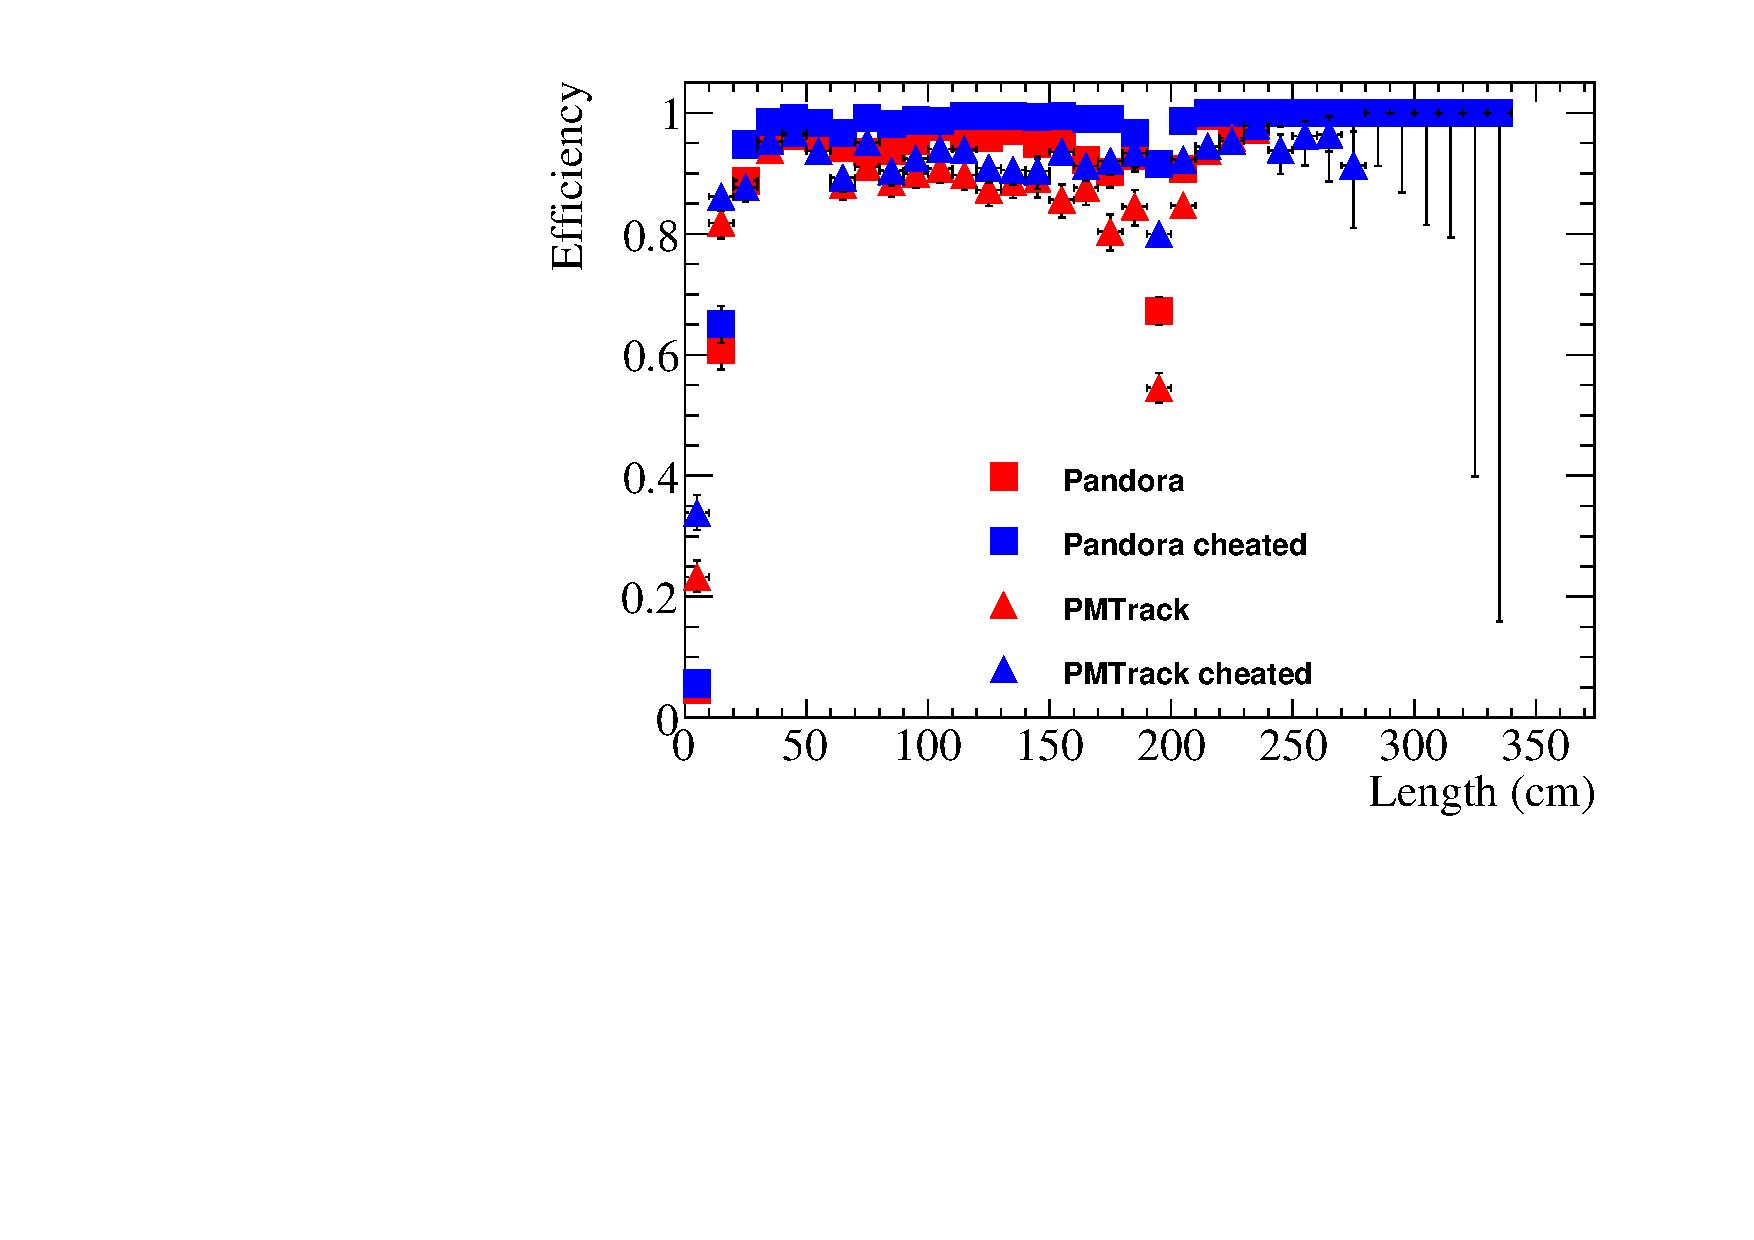
\includegraphics[width=\textwidth]{Effic_AntiMuon_500V_All_Length}
    \caption{Reconstruction efficiencies for an Anti-Muon sample.}
    \label{fig:SimEffic_Length_AMu}
  \end{subfigure}
  \hspace{0.08\textwidth}
  \begin{subfigure}{0.45\textwidth}
    \centering
    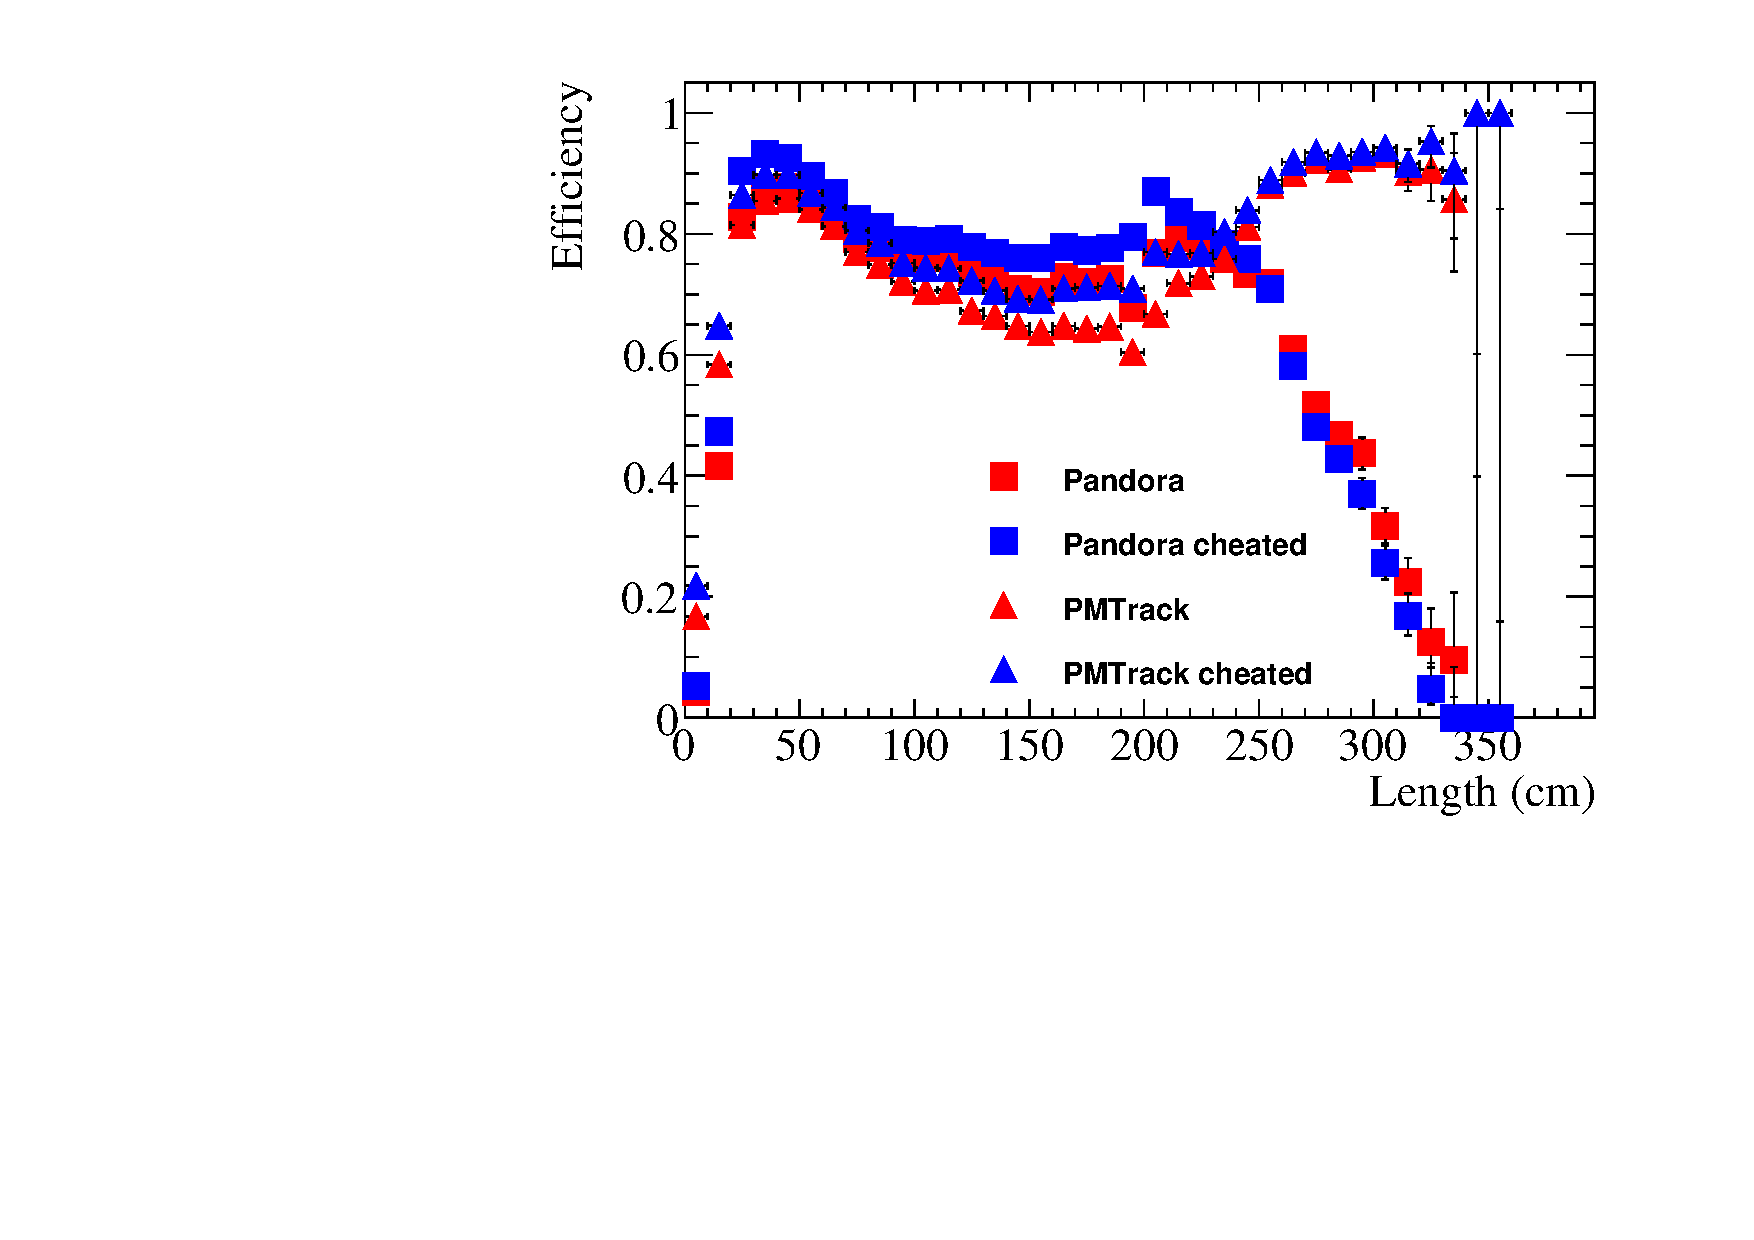
\includegraphics[width=\textwidth]{Effic_Cosmics_500V_All_Length}
    \caption{Reconstruction efficiencies for a CRY sample.}
    \label{fig:SimEffic_Length_CRY}
  \end{subfigure}
  \caption[The reconstruction efficiencies for simulated events as a function of Monte Carlo truth track length.]
          {The reconstruction efficiencies for simulated events as a function of Monte Carlo truth track length. The efficiencies are shown for non-cheated reconstruction (red blocks) and cheated reconstruction (blue blocks) for both Pandora (square blocks) and PMTrack (triangle blocks).}
          \label{fig:SimEffic_Length}
\end{figure}

\begin{figure}[h!]
  \centering
  \begin{subfigure}{0.45\textwidth}
    \centering
    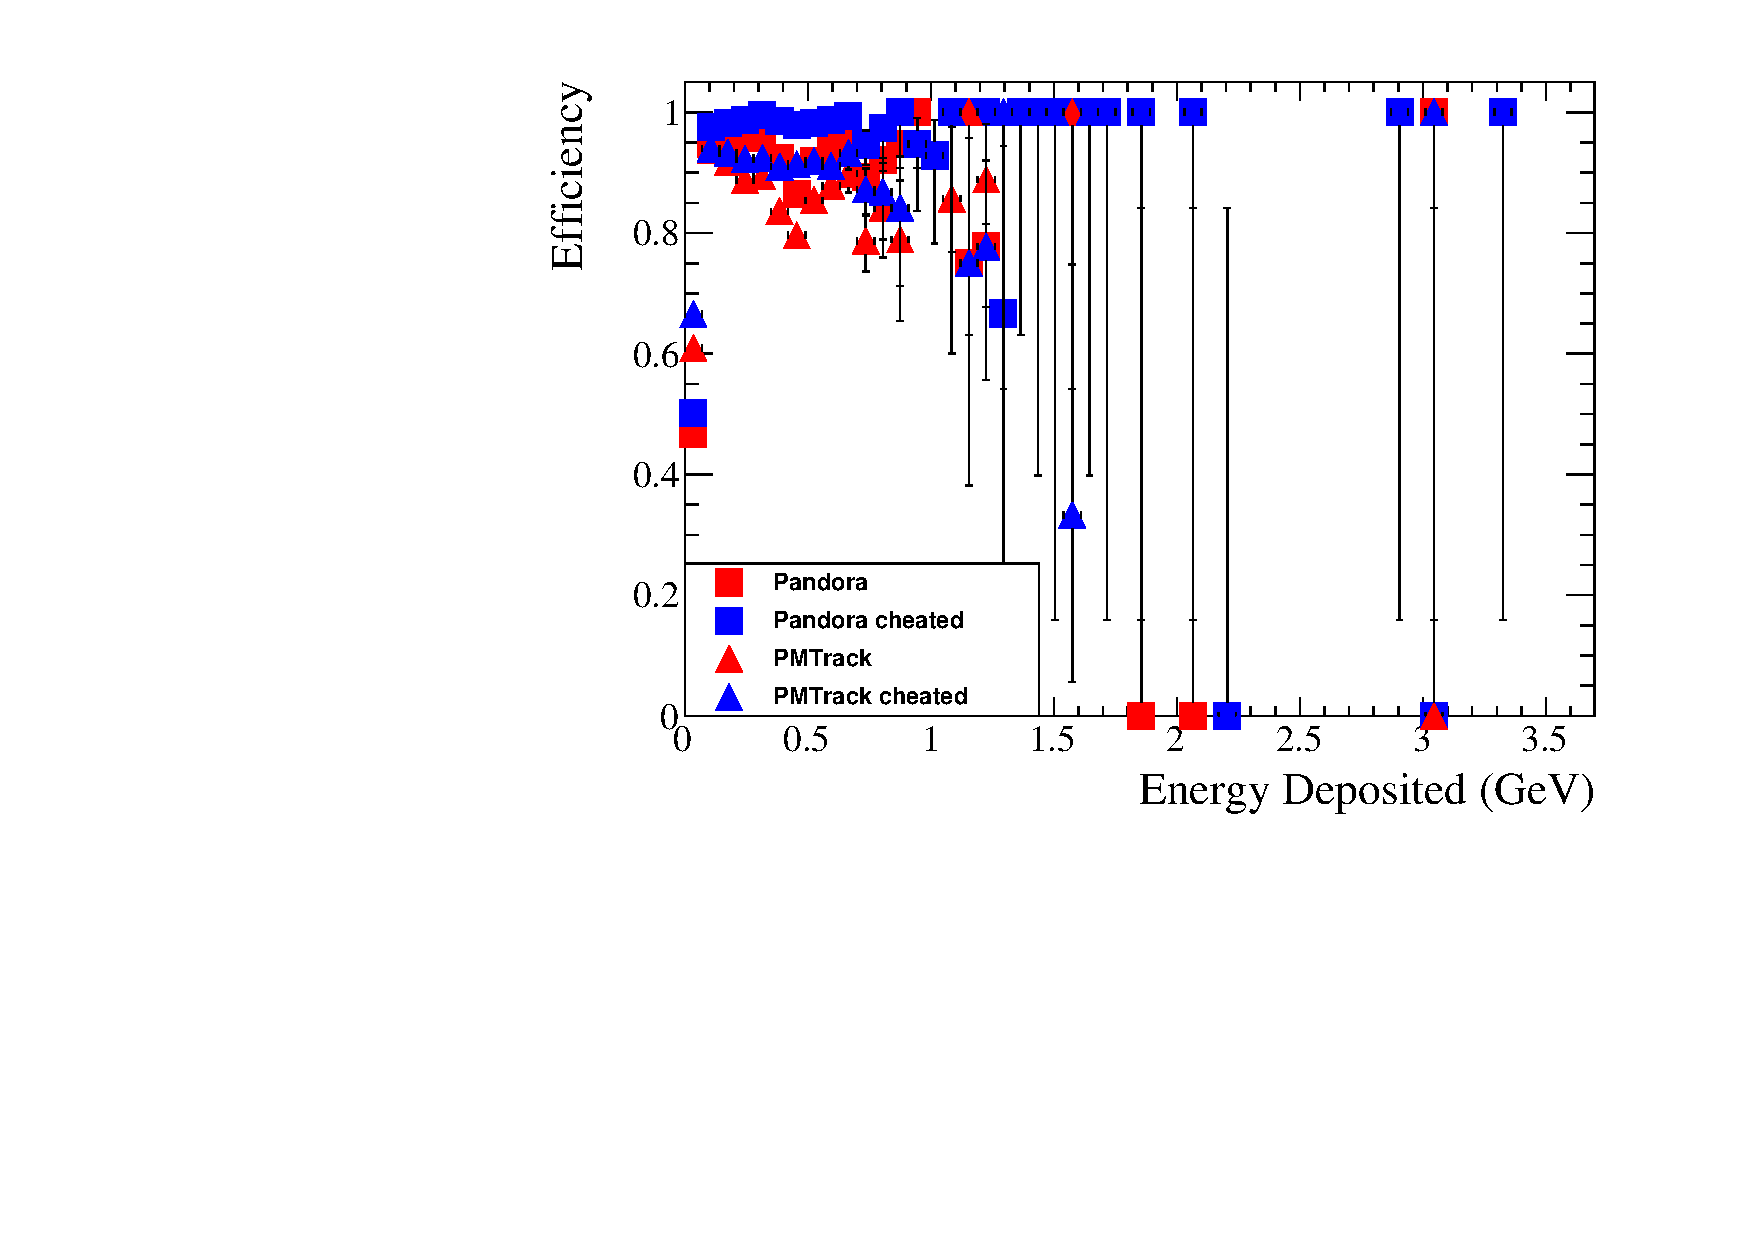
\includegraphics[width=\textwidth]{Effic_AntiMuon_500V_All_EnDepos}
    \caption{Reconstruction efficiencies for an Anti-Muon sample.}
    \label{fig:SimEffic_EnDepos_AMu}
  \end{subfigure}
  \hspace{0.08\textwidth}
  \begin{subfigure}{0.45\textwidth}
    \centering
    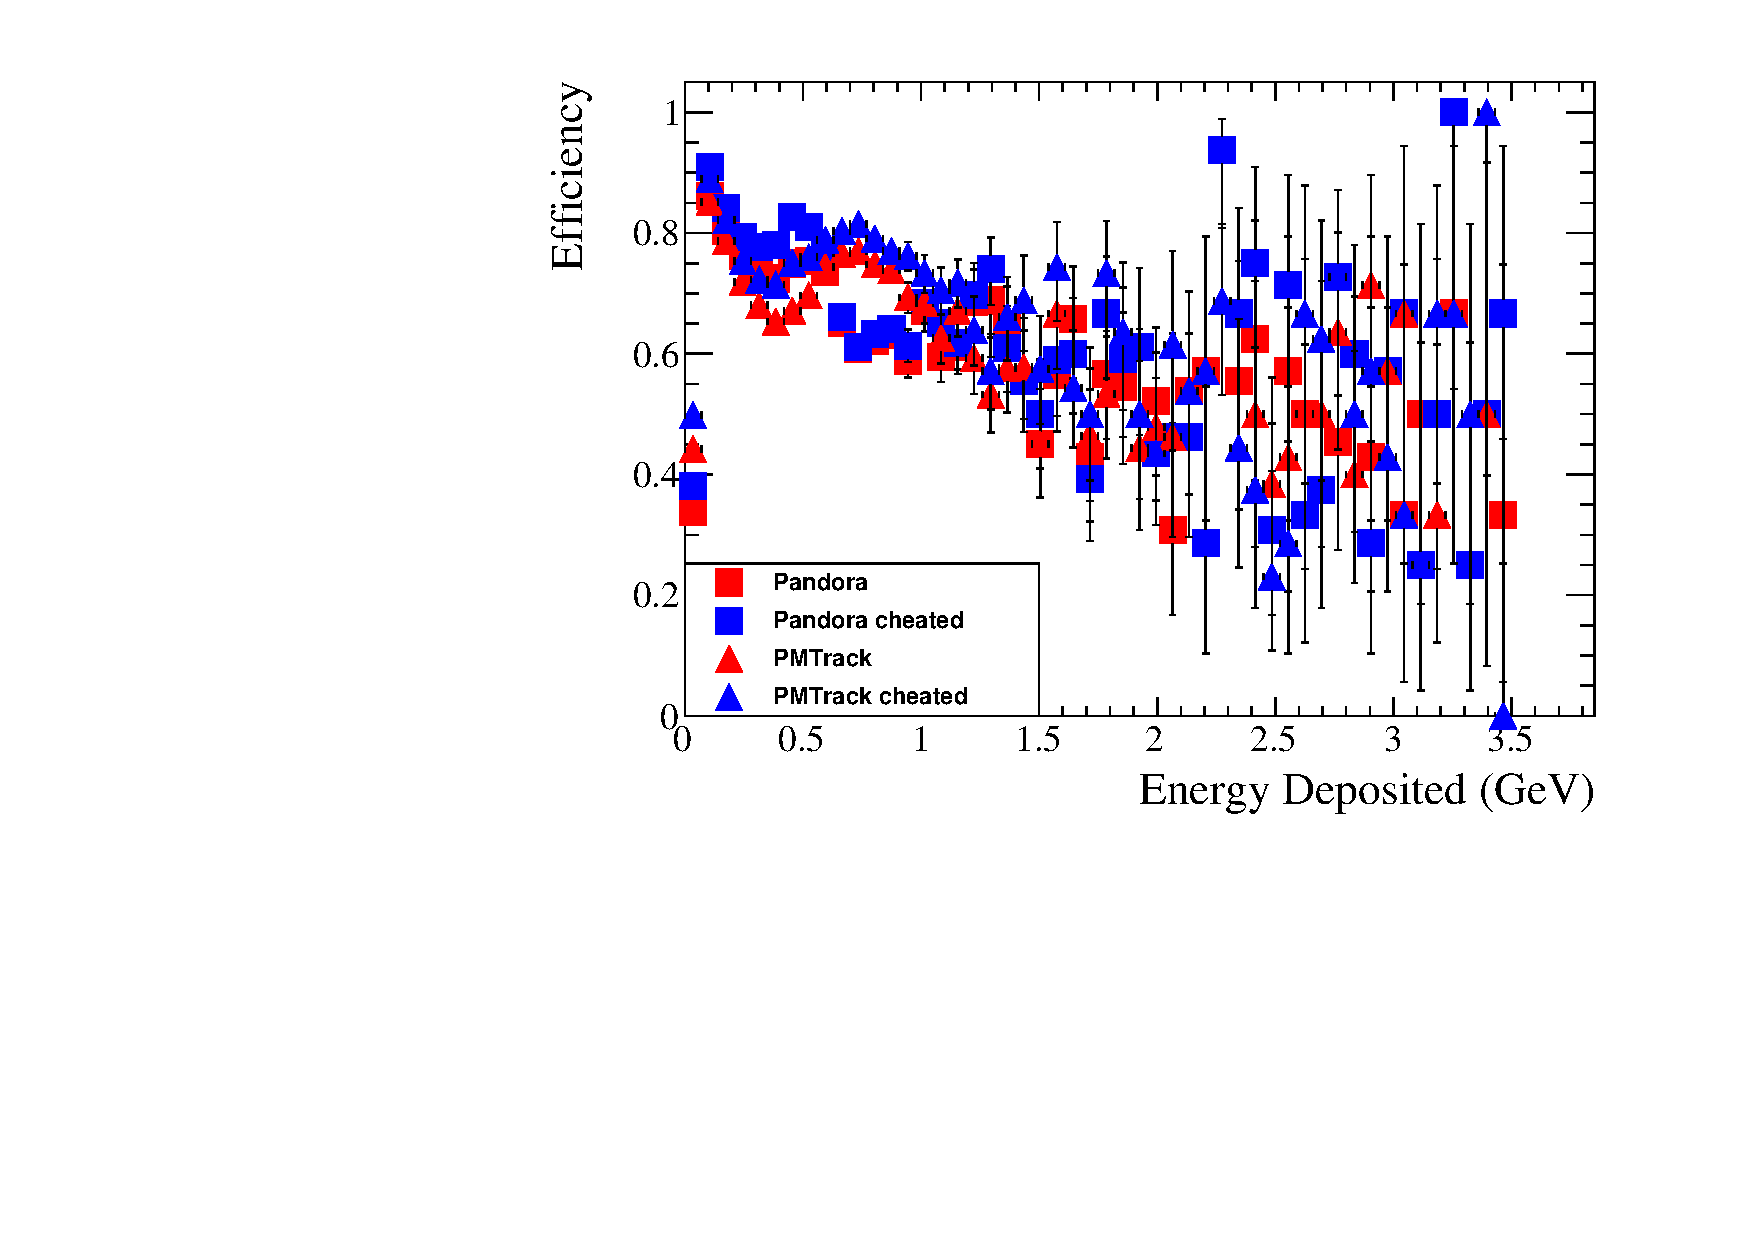
\includegraphics[width=\textwidth]{Effic_Cosmics_500V_All_EnDepos}
    \caption{Reconstruction efficiencies for a CRY sample.}
    \label{fig:SimEffic_EnDepos_CRY}
  \end{subfigure}
  \caption[The reconstruction efficiencies for simulated events as a function of Monte Carlo truth deposited energy.]
          {The reconstruction efficiencies for simulated events as a function of Monte Carlo truth deposited energy. The efficiencies are shown for non-cheated reconstruction (red blocks) and cheated reconstruction (blue blocks) for both Pandora (square blocks) and PMTrack (triangle blocks).}
          \label{fig:SimEffic_EnDepos}
\end{figure}

\begin{figure}[h!]
  \centering
  \begin{subfigure}{0.45\textwidth}
    \centering
    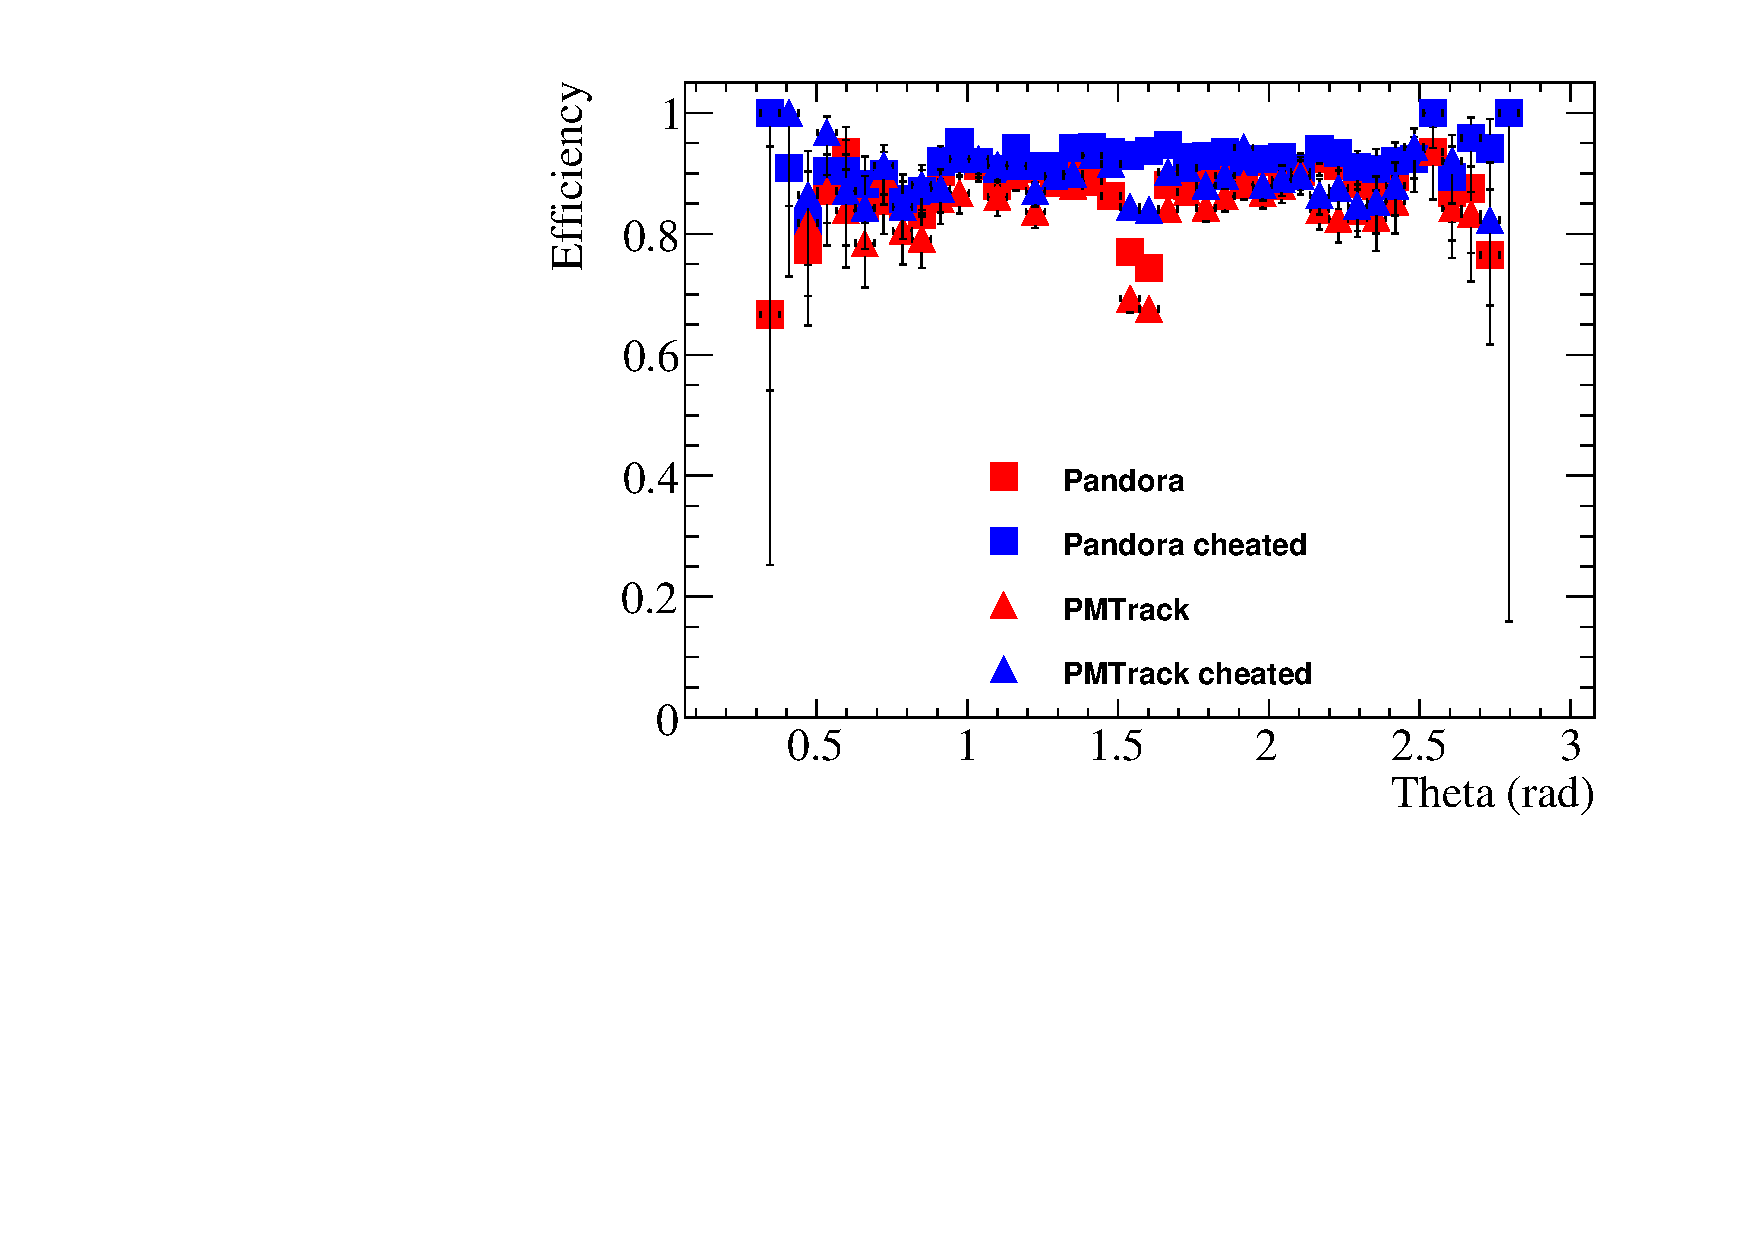
\includegraphics[width=\textwidth]{Effic_AntiMuon_500V_All_Theta}
    \caption{Reconstruction efficiencies for an Anti-Muon sample.}
    \label{fig:SimEffic_Theta_AMu}
  \end{subfigure}
  \hspace{0.08\textwidth}
  \begin{subfigure}{0.45\textwidth}
    \centering
    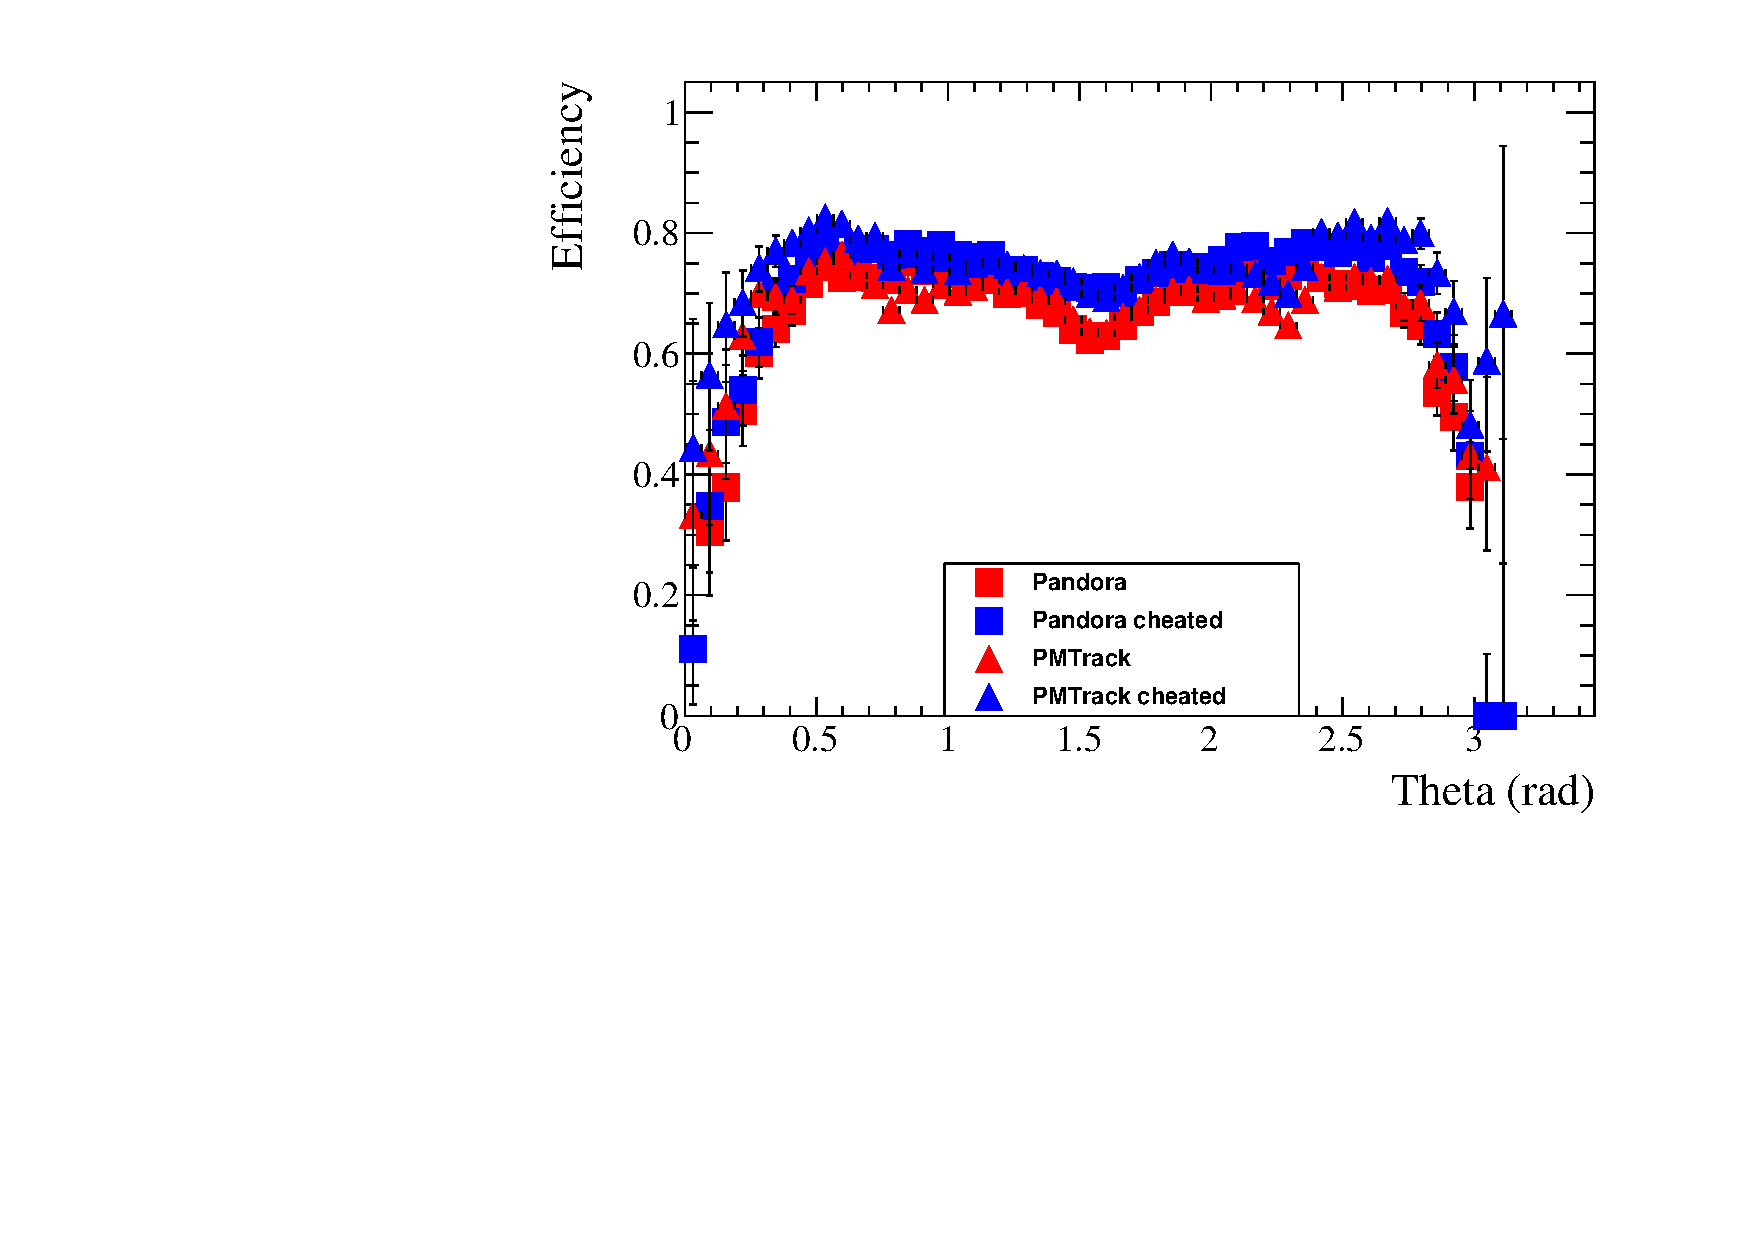
\includegraphics[width=\textwidth]{Effic_Cosmics_500V_All_Theta}
    \caption{Reconstruction efficiencies for a CRY sample.}
    \label{fig:SimEffic_Theta_CRY}
  \end{subfigure}
  \caption[The reconstruction efficiencies for simulated events as a function of Monte Carlo truth track angle in theta.]
          {The reconstruction efficiencies for simulated events as a function of Monte Carlo truth track angle in theta. The efficiencies are shown for non-cheated reconstruction (red blocks) and cheated reconstruction (blue blocks) for both Pandora (square blocks) and PMTrack (triangle blocks).}
          \label{fig:SimEffic_Theta}
\end{figure}

\begin{figure}[h!]
  \centering
  \begin{subfigure}{0.45\textwidth}
    \centering
    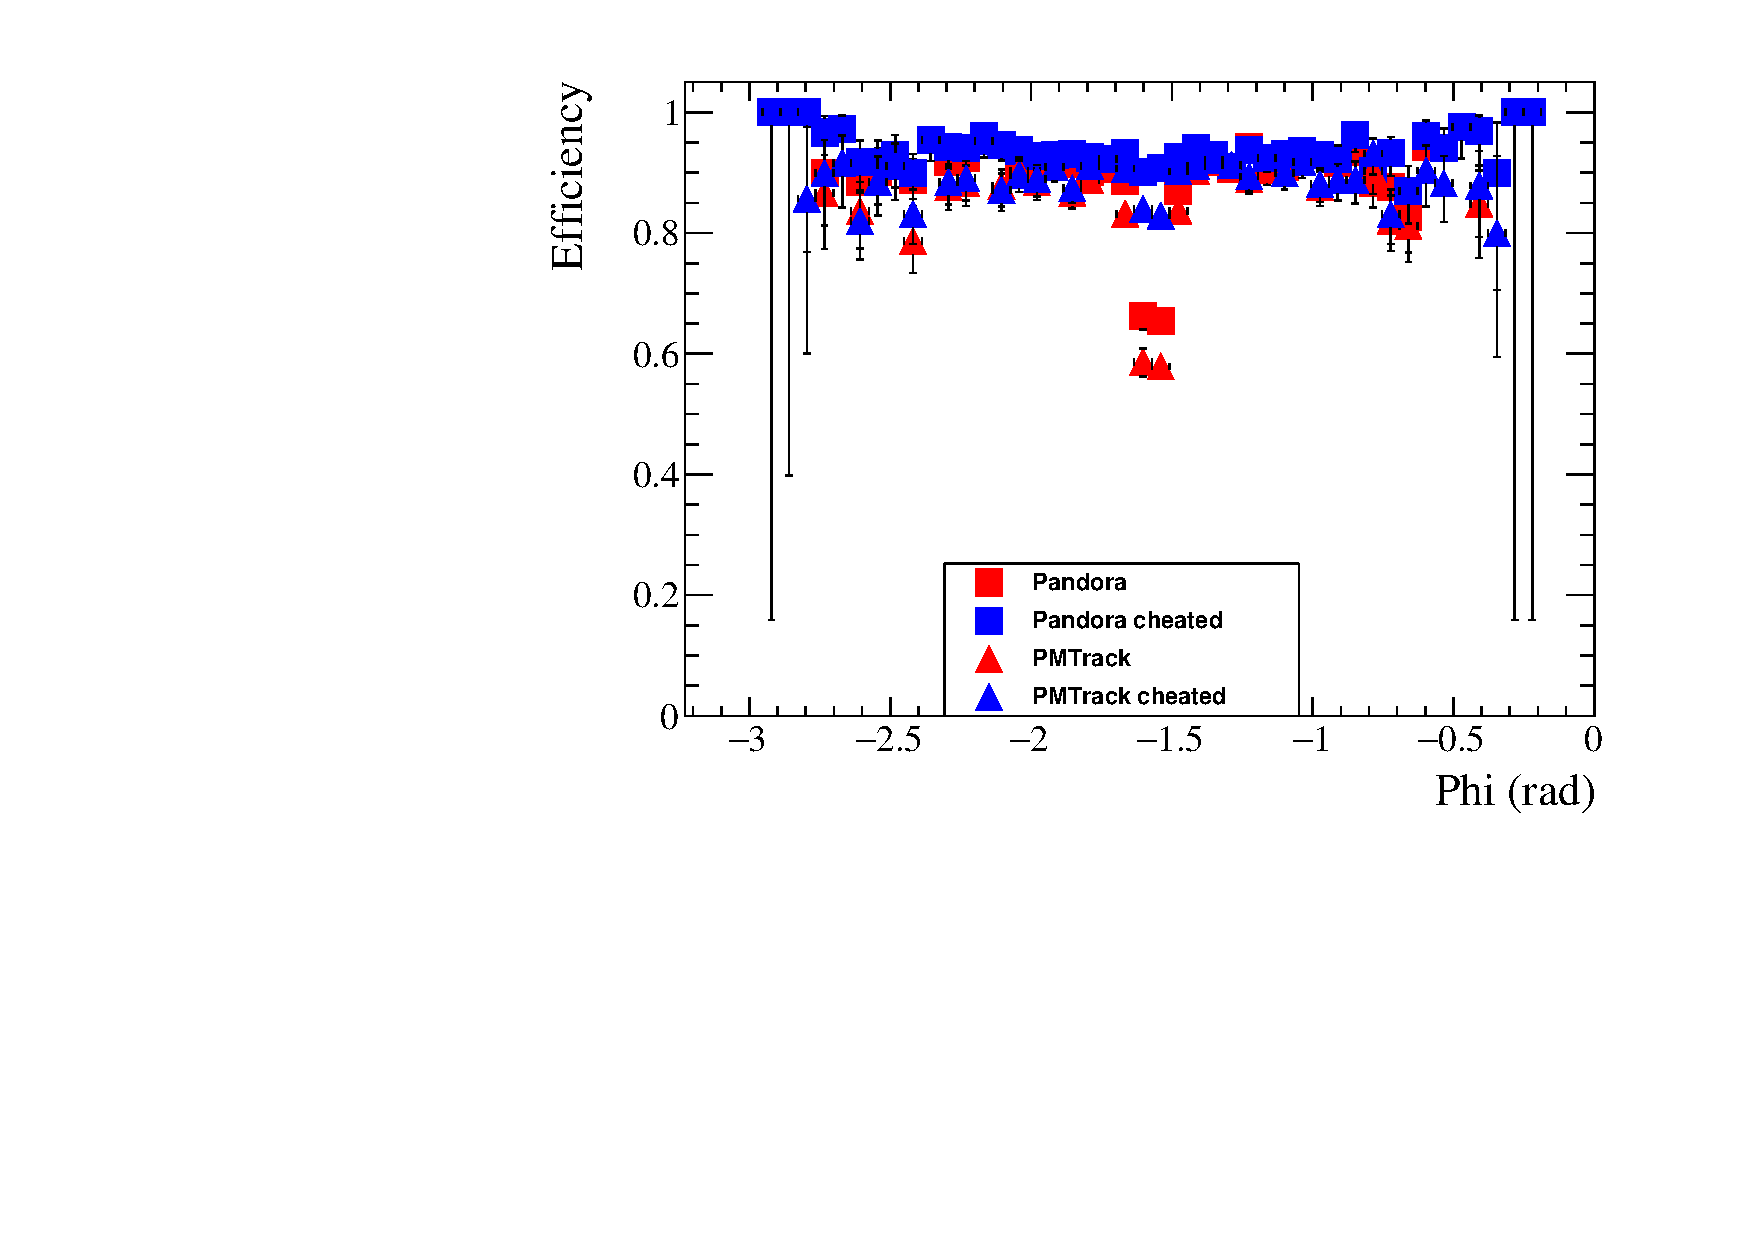
\includegraphics[width=\textwidth]{Effic_AntiMuon_500V_All_Phi}
    \caption{Reconstruction efficiencies for an Anti-Muon sample.}
    \label{fig:SimEffic_Phi_AMu}
  \end{subfigure}
  \hspace{0.08\textwidth}
  \begin{subfigure}{0.45\textwidth}
    \centering
    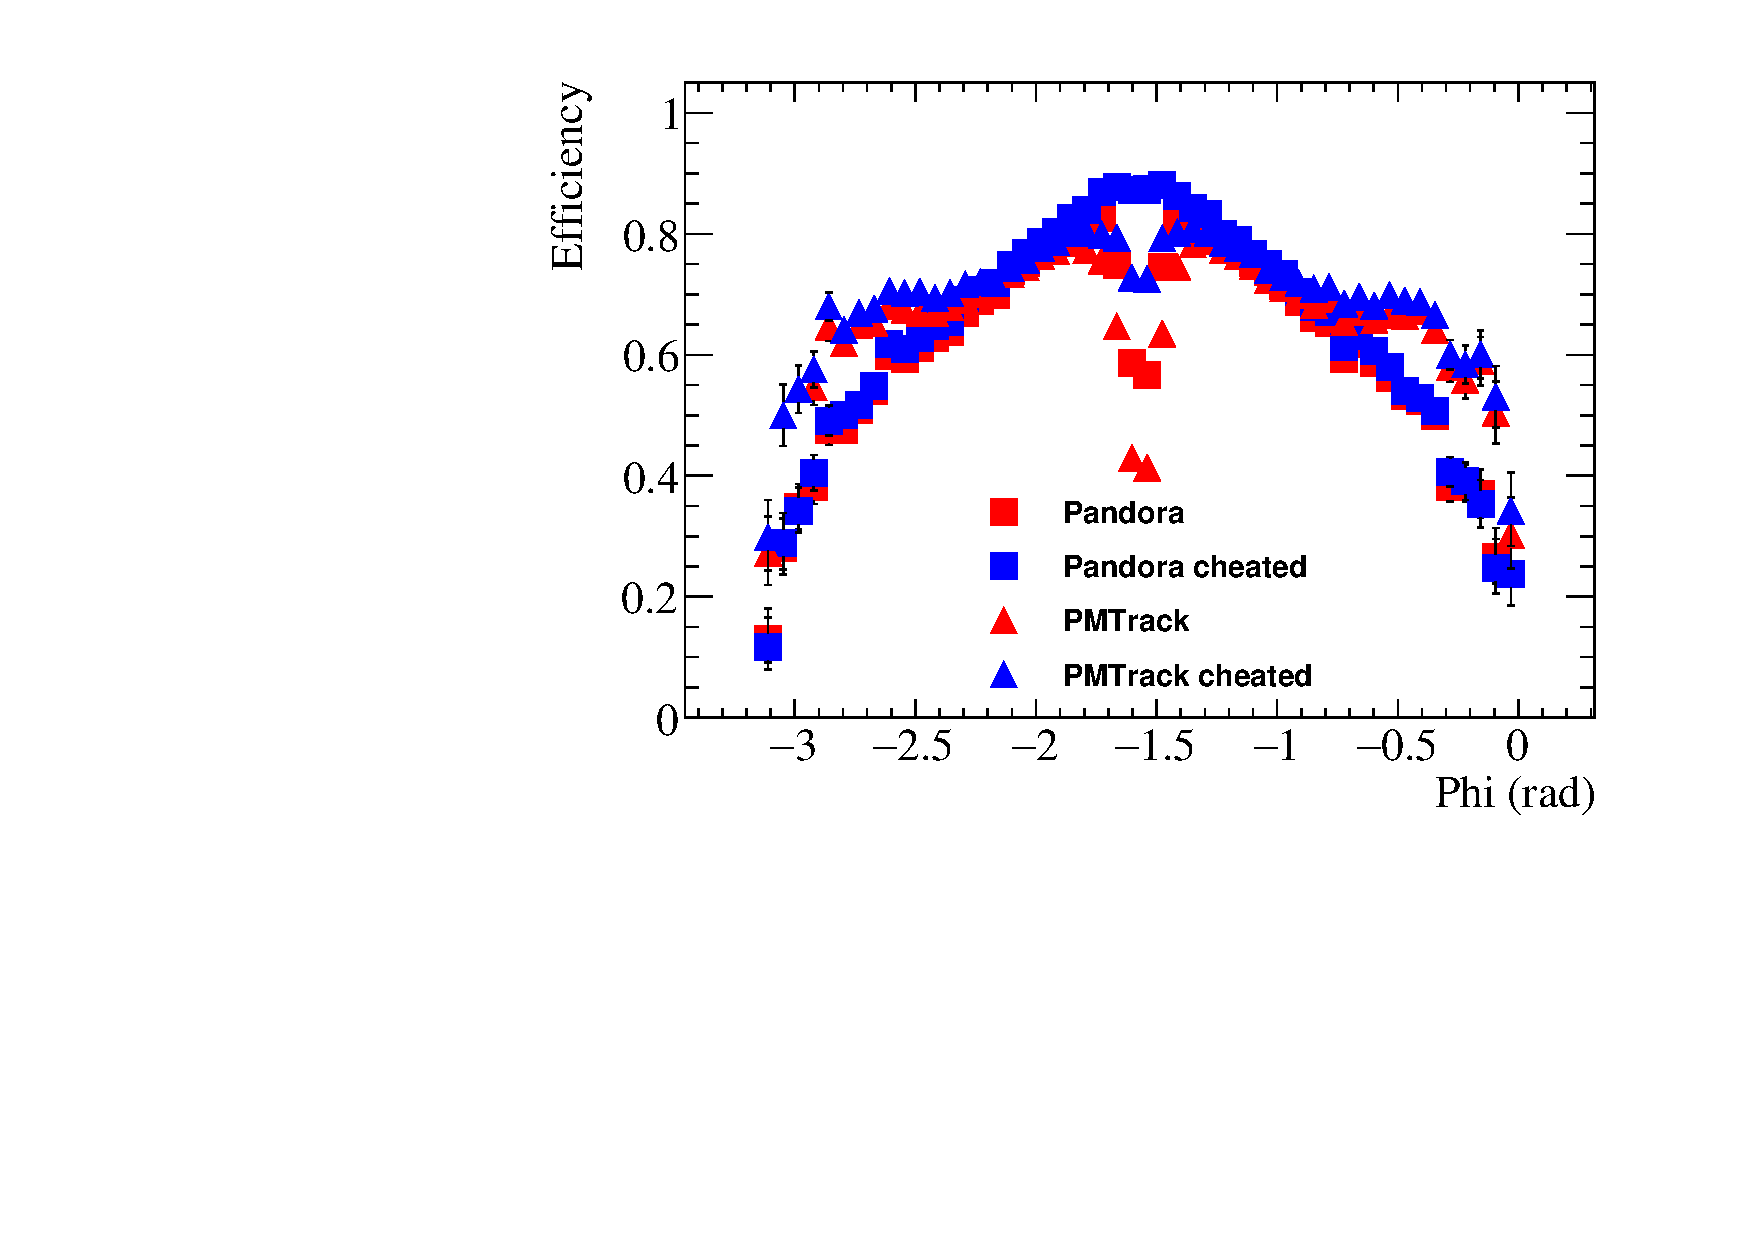
\includegraphics[width=\textwidth]{Effic_Cosmics_500V_All_Phi}
    \caption{Reconstruction efficiencies for a CRY sample.}
    \label{fig:SimEffic_Phi_CRY}
  \end{subfigure}
  \caption[The reconstruction efficiencies for simulated events as a function of Monte Carlo truth track angle in phi.]
          {The reconstruction efficiencies for simulated events as a function of Monte Carlo truth track angle in phi. The efficiencies are shown for non-cheated reconstruction (red blocks) and cheated reconstruction (blue blocks) for both Pandora (square blocks) and PMTrack (triangle blocks).}
          \label{fig:SimEffic_Phi}
\end{figure}

\begin{figure}[h!]
  \centering
  \begin{subfigure}{0.45\textwidth}
    \centering
    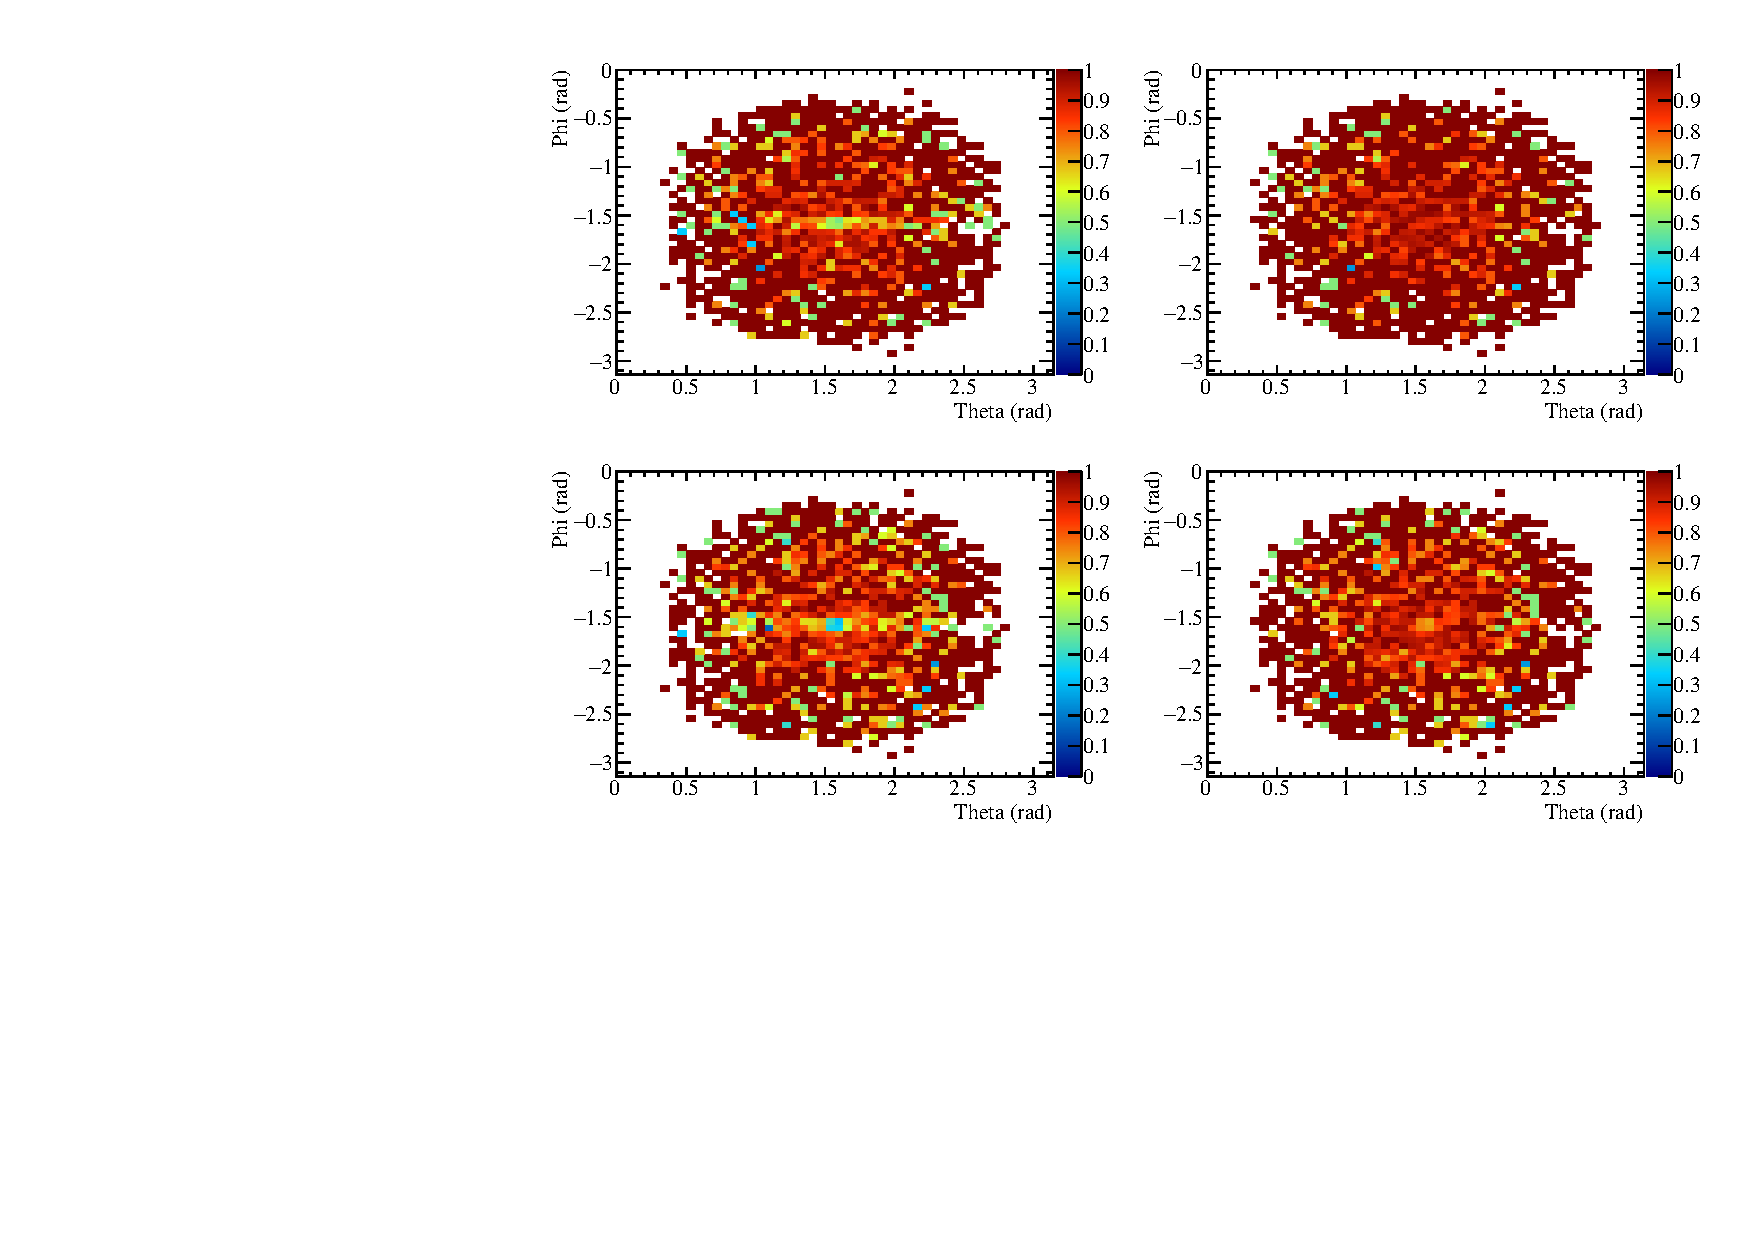
\includegraphics[width=\textwidth]{Effic_AntiMuon_500V_All_PhiTheta}
    \caption{Reconstruction efficiencies for an Anti-Muon sample.}
    \label{fig:SimEffic_ThetaPhi_AMu}
  \end{subfigure}
  \hspace{0.08\textwidth}
  \begin{subfigure}{0.45\textwidth}
    \centering
    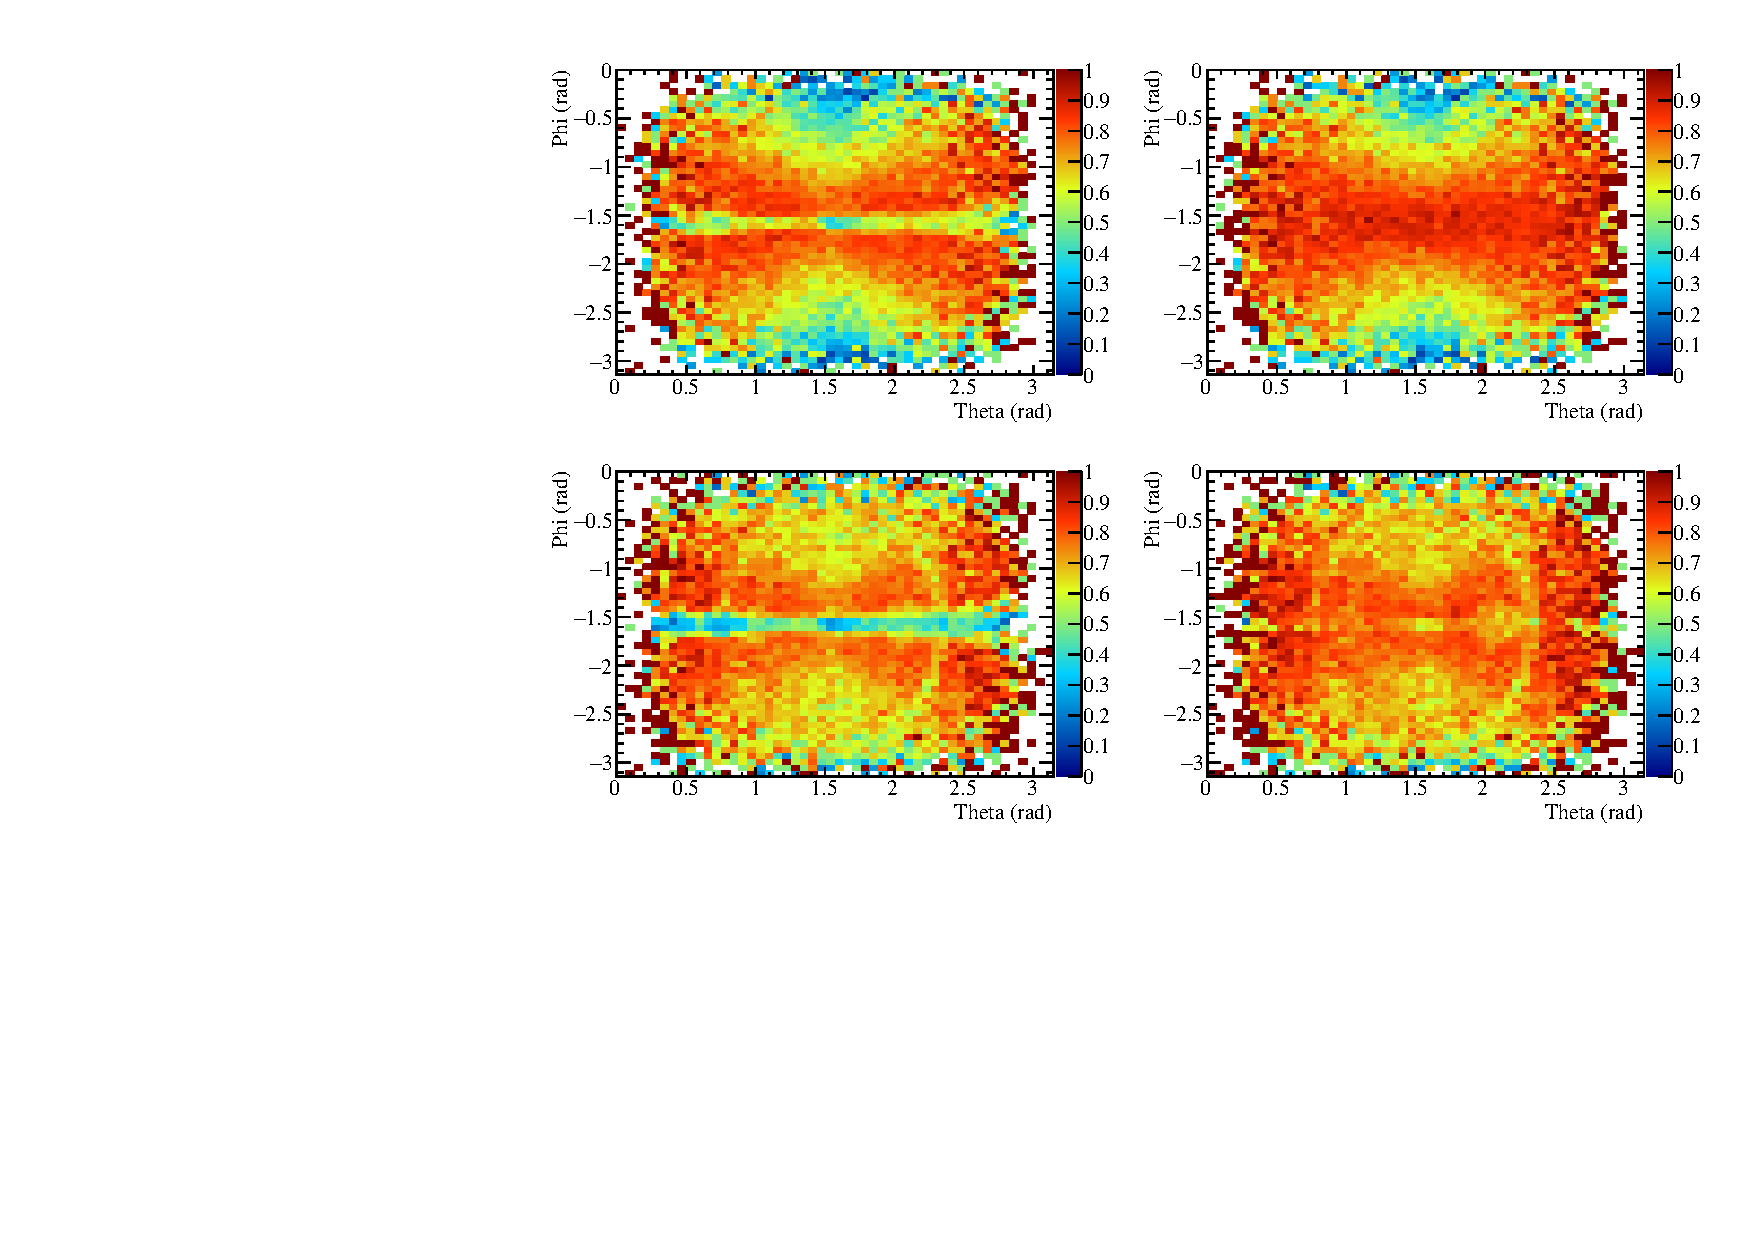
\includegraphics[width=\textwidth]{Effic_Cosmics_500V_All_PhiTheta}
    \caption{Reconstruction efficiencies for a CRY sample.}
    \label{fig:SimEffic_ThetaPhi_CRY}
  \end{subfigure}
  \caption[The reconstruction efficiencies for simulated events as a function of Monte Carlo truth track angle in theta and phi.]
          {The reconstruction efficiencies for simulated events as a function of Monte Carlo truth track angle in theta and phi. The efficiencies are shown for non-cheated reconstruction (plots on the left) and cheated reconstruction (plots on the right) for both Pandora (plots on the top) and PMTrack (plots on the bottom).}
          \label{fig:SimEffic_ThetaPhi}
\end{figure}

A striking feature of Figure~\ref{fig:SimEffic_Length} is the rapid decrease in reconstructed efficiency for the CRY sample for track lengths above 250 cm when using Pandora. The cause of this is that tracks are reconstructed separately in the long and short drift volumes before being merged when they are found to be co-linear in the $yz$ plane. This is not a problem in the Anti-Muon sample as the $x$ position of the hits calculated using Equation~\ref{eq:HitTime} will be correct. However, when the same is done for hits in the CRY sample using particles with large interaction times the $x$ positions will have offsets proportional to the interaction time unless the hit time is corrected by Equation~\ref{eq:HitTime_Int}. The result of this is that merged tracks can have discontinuities in their $x$ coordinates of more than 20 m. As the interaction time of the track is calculated using the output of the tracking algorithms it is not possible to directly correct for the interaction time at present. It is however possible to subtract this jump in $x$ position from the track length quantity which is calculated when the stitched track is stored in the event, this will give the correct track length though the user will still have to correct individual hit positions in later analyses using the calculated interaction time. This is what is done by PMTrack, hence it not exhibiting this rapid decrease in reconstruction efficiency for long tracks. \\

\begin{subequations} \begin{align}
  x_{Hit} &= T_{Hit} \times v_{Drift} \label{eq:HitTime} \\
  T_{Hit} &= T_{Measured} - T_{Interaction} \label{eq:HitTime_Int}
\end{align} \end{subequations}

It is clear from Figure~\ref{fig:SimEffic_Length} that tracks of lengths less than 30 cm are poorly reconstructed. The very low efficiency for tracks with lengths less than 10 cm can be partially attributed to particles with lengths of less than 1 cm as these particles, which represent ~30\% of the particles with lengths below 10 cm, are too short to be reconstructed using the current reconstruction process. These particles will need to be reconstructed when looking for supernovae bursts though special algorithms will be written to do this, as the traditional hit finding and clustering algorithms may discard them due to the isolated nature of the hits. Another issue is that the low energies of these particles may mean that the signals that they produce are below threshold and so will not even be reconstructed, or if hits are reconstructed they may be too close to a more energetic track and get absorbed into them. The reconstruction of tracks is affected by the number of wires which they cross, though this should not matter for particles with lengths of more than 5 cm as they will have crossed roughly 10 wires in each plane which should produce enough unique hits for a cluster to be reliably constructed. This can be seen to be the case for PMTrack when considering the Anti-Muon sample, as the efficiency for track lengths between 10 and 20 cm is roughly the same as that for track lengths between 20 and 30 cm, however when considering the CRY sample there is still a significant decrease in efficiency. This is attributed to the more complex event structure in the CRY sample, where secondary particles are produced which are mis-reconstructed even though they travel reasonable distances. This is can be seen to be the case as when only primary muons in the CRY sample are considered the reconstruction efficiency is seen to be the same as that for the Anti-Muon sample. \\

The trend of increasing efficiency for longer track lengths from Figure~\ref{fig:SimEffic_Length} can also be seen in Figure~\ref{fig:SimEffic_EnDepos} as the energy deposited increases. This is because particles which deposit more energy will tend to have travelled further in the detector. The amount of energy that particles deposit is limited by the size of the detector though as particles with an energy of more than 1 GeV are energetic enough to through-going MIPS. This results in few particles depositing more than 1 GeV in the detector causing the uncertainty in the reconstruction efficiency to increase above this energy. The increased statistics at high despoited energies in Figure~\ref{fig:SimEffic_EnDepos_CRY} is due to the larger number of muons generated in the CRY which create large electromagnetic showers showers when they enter the LAr. \\

It is also interesting to note the pronounced decreases in reconstruction efficiencies for particular angles shown in Figure~\ref{fig:SimEffic_Theta} and Figure~\ref{fig:SimEffic_Phi}. The decrease in efficiency at $\phi = \frac{\pi}{2}$ can be attributed to the drop in efficiency for tracks of ~200 cm, as this corresponds to the vertical height of the detector meaning that few collection wires are hit and so determining the triple points needed by the disambiguation are difficult to find. This is verified by the large increase in efficiency achieved by cheating the disambiguation. Similarly the decrease in efficiency at $\theta = \frac{\pi}{2}$ can be attributed to particles which are perpendicular to the collection wires resulting in few collection wires being hit. \\  

The information from Figures~\ref{fig:SimEffic_Theta} and~\ref{fig:SimEffic_Phi} is combined in Figure~\ref{fig:SimEffic_ThetaPhi} where the sharp drops in efficiency for the CRY sample are particularly visible. The effect of cheated disambiguation is clear in Figure~\ref{fig:SimEffic_ThetaPhi_CRY} where the dip in efficiency as a function of $\theta$ at fixed $\phi=\frac{\pi}{2}$ is completely removed. The same is not true for the dip in efficiency as a function $\phi$ at fixed $\theta = \frac{\pi}{2}$, though the reduction in efficiency was not uniform or as severe across all values of $\theta$ as it remains mainly confined to values of $\theta$ close to 0 or $\pi$, particularly when using Pandora . The observation that a significant improvement in the quality of reconstruction can be made in improving the disambiguation is a driving force in the wire pitches being 36$^{\circ}$ for the DUNE FD as opposed 45$\pm$0.7$^{\circ}$ in the 35 ton, because as discussed in Section~\ref{sec:LArSoft} the shallower wire pitch makes disambiguation easier. Though disambiguation will be easier in the different geometry, further efforts to improve disambiguation are still required, as are continued efforts to reconstruct the shortest tracks. \\

%********************************** % Fourth Section  *************************************
\section{Performing particle identification}  \label{sec:PID} %Section - X.4
Being able to perform reliable particle identification (PID) is a key requirement for the DUNE experiment, and so efforts have been made to establish a metric by which this can be achieved. The predominant method of performing PID in LAr is to use the relationship between $\frac{dE}{dx}$ and the residual range of the track, defined as being the distance between a point on the track and the stopping point of the track. This relationship is observed to be dependent on particle mass and is quantified by the Bethe-Bloch equation~\citep{Bethe}~\citep{Bloch} which is shown in Figure~\ref{fig:BetheBloch}. The sharp increase in energy loss per unit length can be seen to occur at different momenta for different particle masses meaning that the peak value of $\frac{dE}{dx}$ can change significantly. One example of a large change in the peak value of $\frac{dE}{dx}$ can be seen by comparing muons and protons, whist muons and pions are very similar. \\

\begin{figure}[h!]
  \centering
  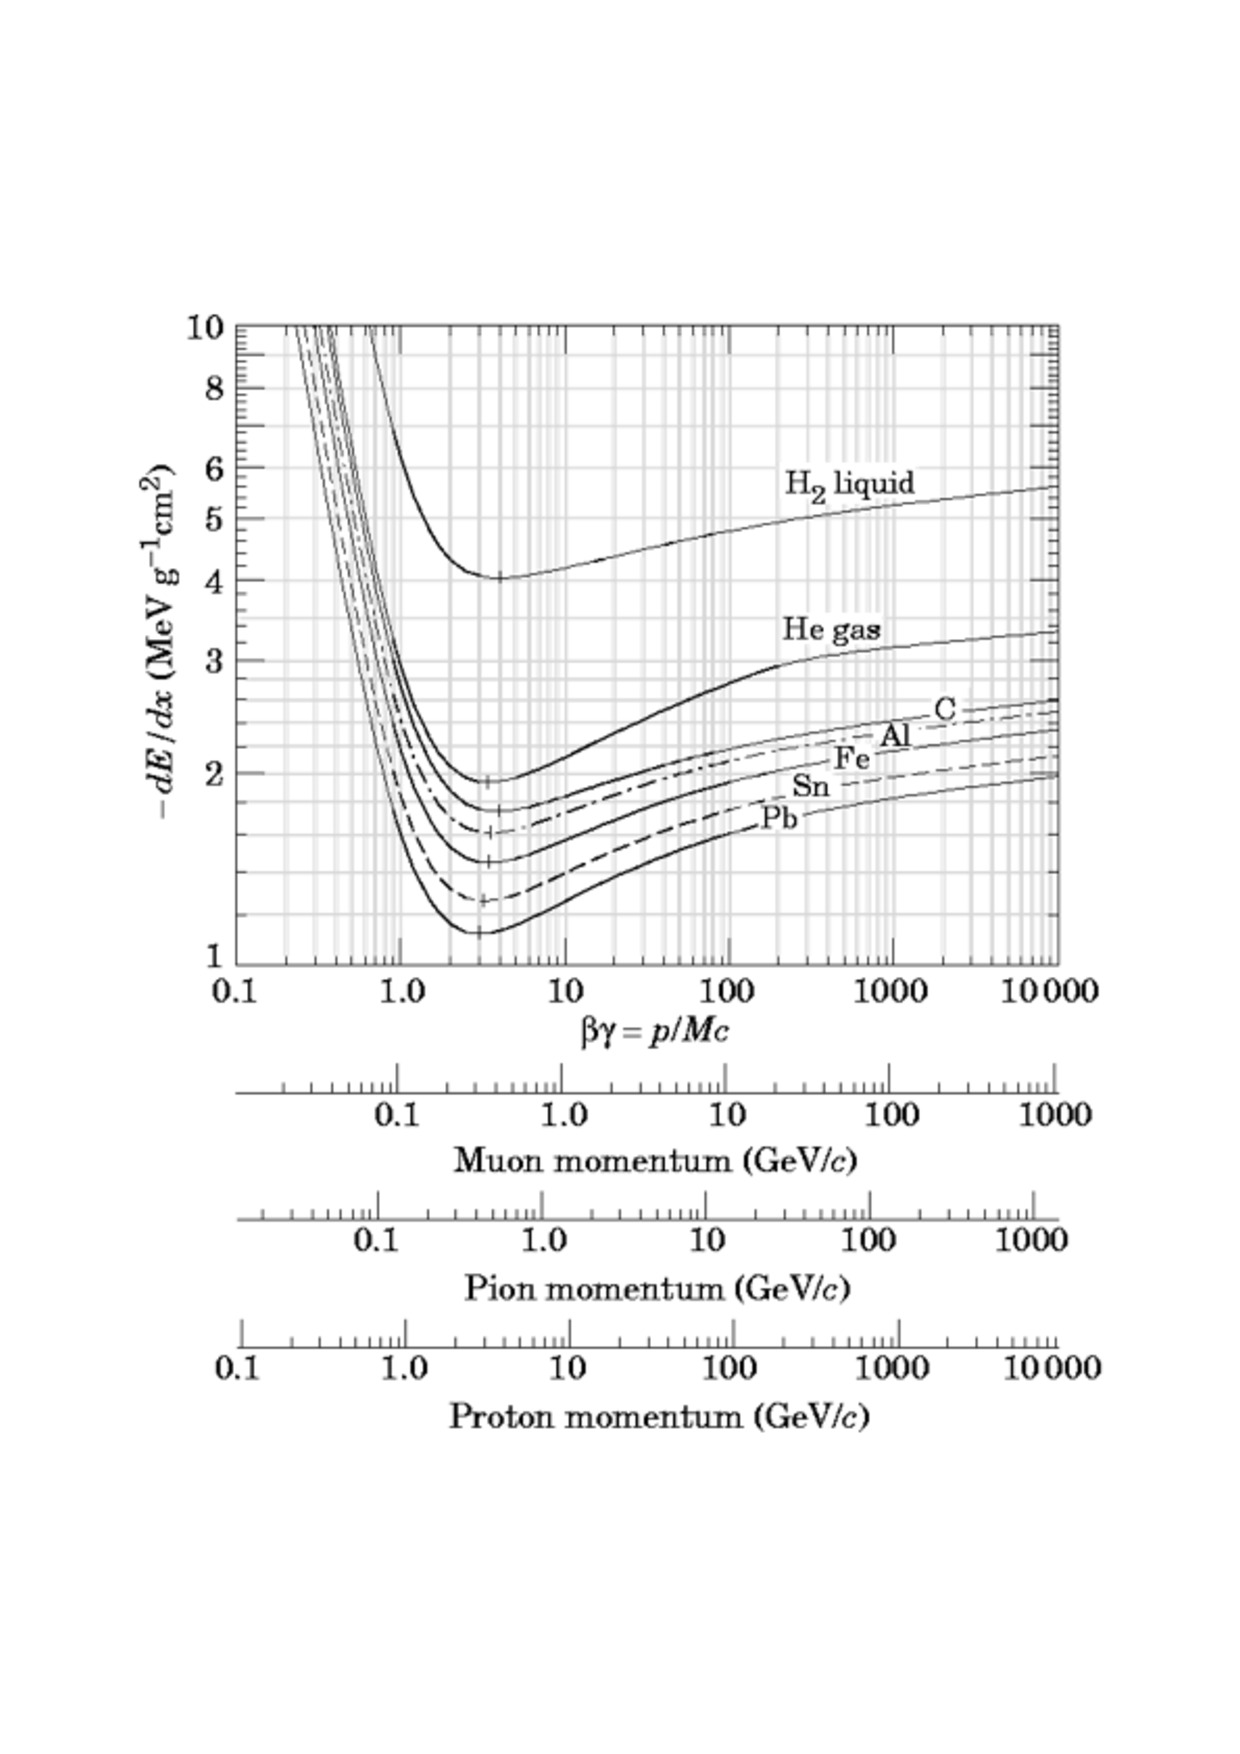
\includegraphics[width=0.5\textwidth]{BetheBlock}
  \caption[The medium and particle type dependence of the Bethe-Bloch equation]
          {The Bethe-Bloch equation describes energy loss per unit length as a function of energy in different mediums. The energy losses expected for different particle types is shown in different mediums. Liquid Argon with a density of 1.4 g cm$^{-3}$ has a density slightly less than that of Carbon at 1.8 g cm$^{-3}$.}
  \label{fig:BetheBloch}
\end{figure}

The particle mass dependence can be seen by plotting the $\frac{dE}{dx}$ against the residual range of the particle on a log-log plot, as shown in Figure~\ref{fig:PIDA_loglog}. A power law dependence is found to describe the relationship~\citep{PIDA_Paper}, as shown in Equation~\ref{eq:PIDA}. The dependence on $b$ is found to be weak, and so can be set to -0.42 for all particle masses. This means that the main discriminant used is the $A$ parameter, which has a strong dependence on particle mass. The values for $A$ and $b$ calculated from Figure~\ref{fig:PIDA_loglog} are shown in Table~\ref{tab:PIDAVals}. It is found that the error introduced by fixing the $b$ parameter is small compared to the error from ionisation fluctuations. \\

\begin{equation}
  \label{eq:PIDA}
  \frac{dE}{dx}_{calo} = A R^b
\end{equation}

\begin{equation}
  \label{eq:PIDA_A}
  A_i = (\frac{dE}{dx}_{calo})_i \times R^{0.42}_i
\end{equation}

\begin{table}
\caption[Stopping power parameterization for various particle types in liquid Argon]
        {Stopping power parameterization for various particle types in LAr~\citep{PIDA_Paper}.}
\centering
\label{tab:PIDAVals}
\begin{tabular}{l c c}
\toprule
{Particle} & {A MeV cm$^{-(1-b)}$} & {b} \\ 
\midrule
Pion     & 8  & -0.37 \\

Kaon     & 14 & -0.41 \\

Proton   & 17 & -0.42 \\

Deuteron & 25 & -0.43 \\
\bottomrule
\end{tabular}
\end{table}

Once the $b$ parameter is set to be constant for all particle types it is possible to calculate a value for the $A$ parameter for each hit on the track using Equation~\ref{eq:PIDA_A}, where $R_i$ is the residual range of the track at that point. The particle type discriminant, called PIDA, can then be calculated for a track by finding the average value of $A_i$ for the track. As the particle mass dependant increase in $\frac{dE}{dx}$ only occurs near the end of the track, the PIDA variable can only be calculated for particles which stop in the detector as all other particles will have MIP-like $\frac{dE}{dx}$ distributions and so cannot be identified in this way. As shown by the plotted range of Figure~\ref{fig:PIDA_loglog} the average value of $A$ is normally calculated for the last 30 cm of the track. \\

The PIDA method was tested in~\citep{PIDA_Paper}, where the PIDA values were calculated for Monte Carlo particles which stopped in the detector using truth information over the last 30 cm of the particle lengths. This is shown in Figure~\ref{fig:PIDA_MC}, where a clear separation can be seen between the peaks for Muons, Pions, Kaons and Protons. Though the Muon and Pion peaks are relatively close together they can still be resolved in the plot due to little overlap. It is interesting to note how tight the PIDA distributions found in the paper are, which allows the different particles types to cleanly separated in the truth study. The author notes that an incorrect tuning of the recombination effects will cause the distributions to become broader, and an incorrect calibration of the detector will introduce a systematic shift in the expected values of PIDA. \\

\begin{figure}[h!]
  \centering
  \begin{subfigure}{0.45\textwidth}
    \centering
    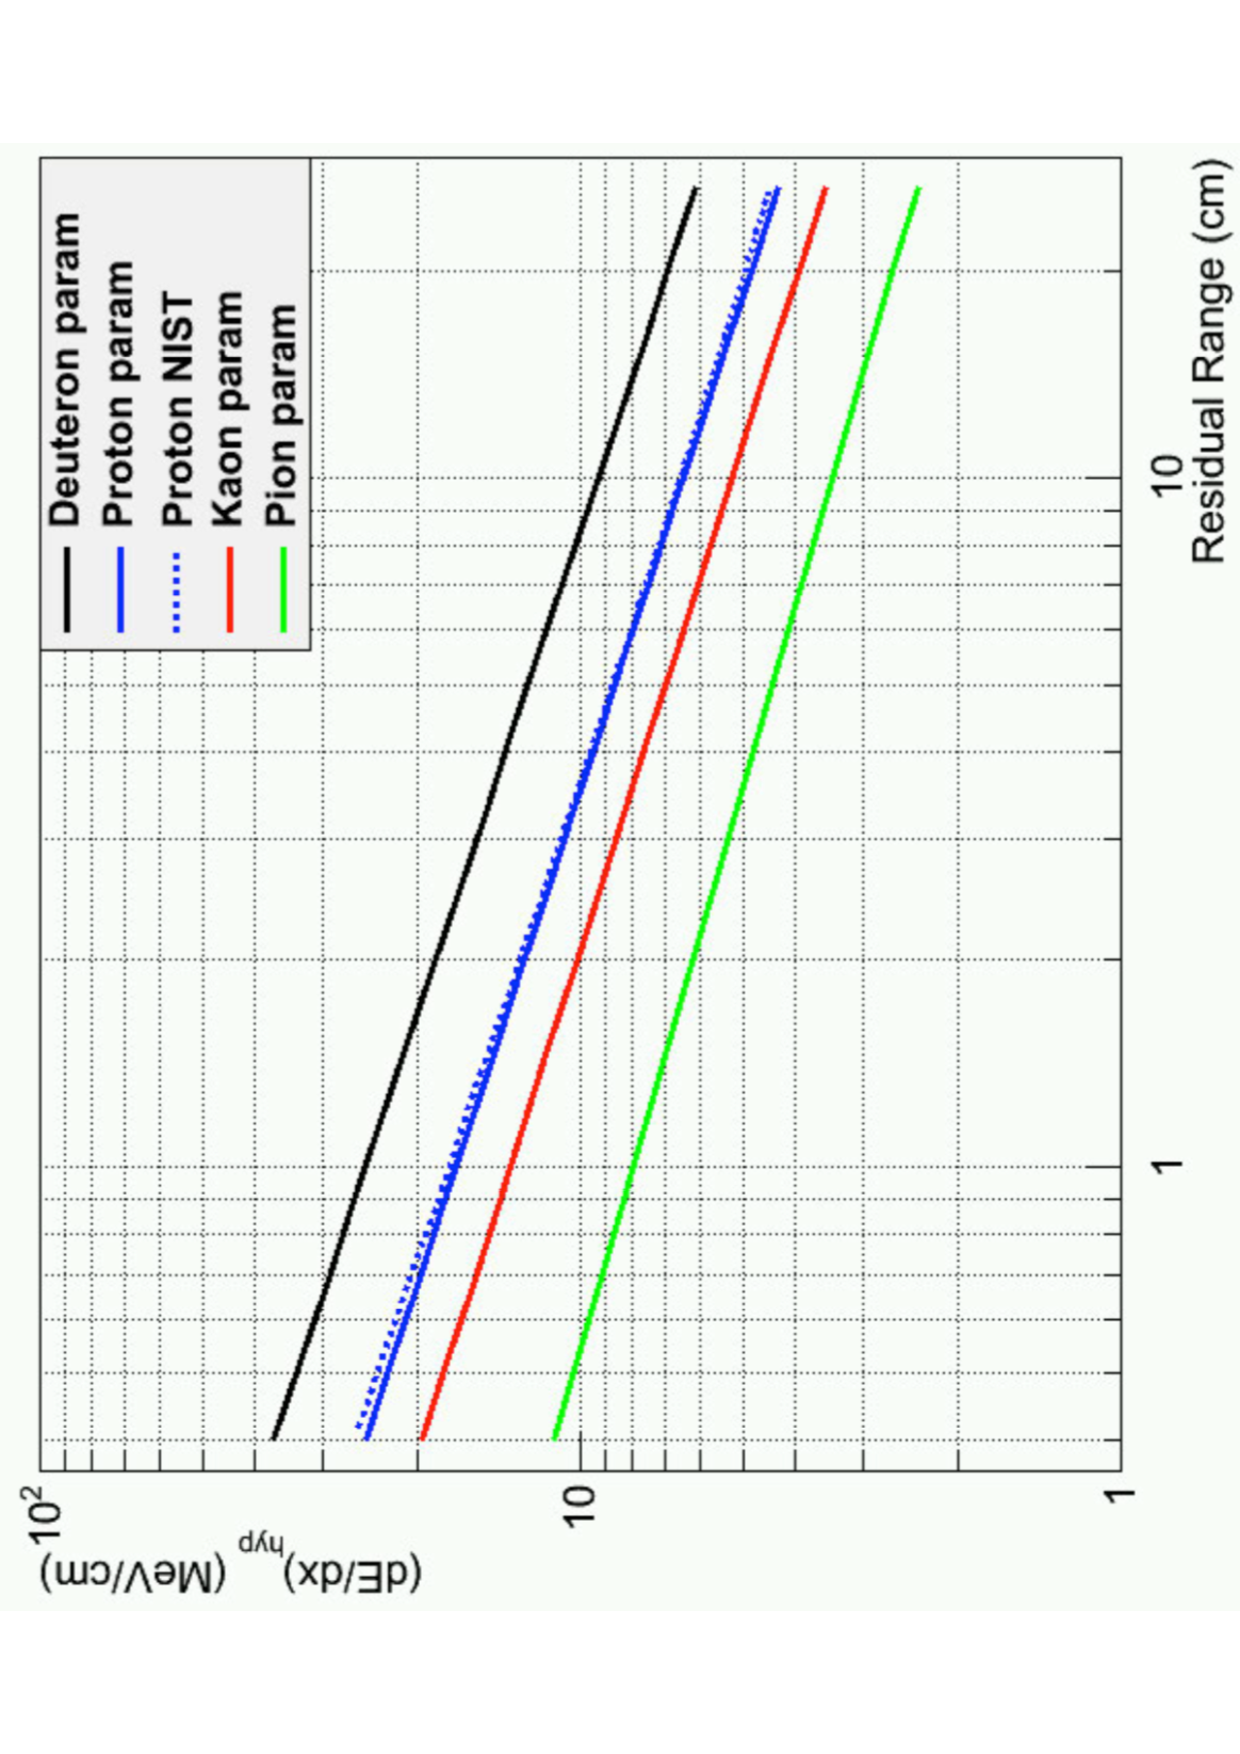
\includegraphics[width=\textwidth]{StoppingPower}
    \caption{Stopping power for different particle masses.}
    \label{fig:PIDA_loglog}
  \end{subfigure}
  \hspace{0.08\textwidth}
  \begin{subfigure}{0.45\textwidth}
    \centering
    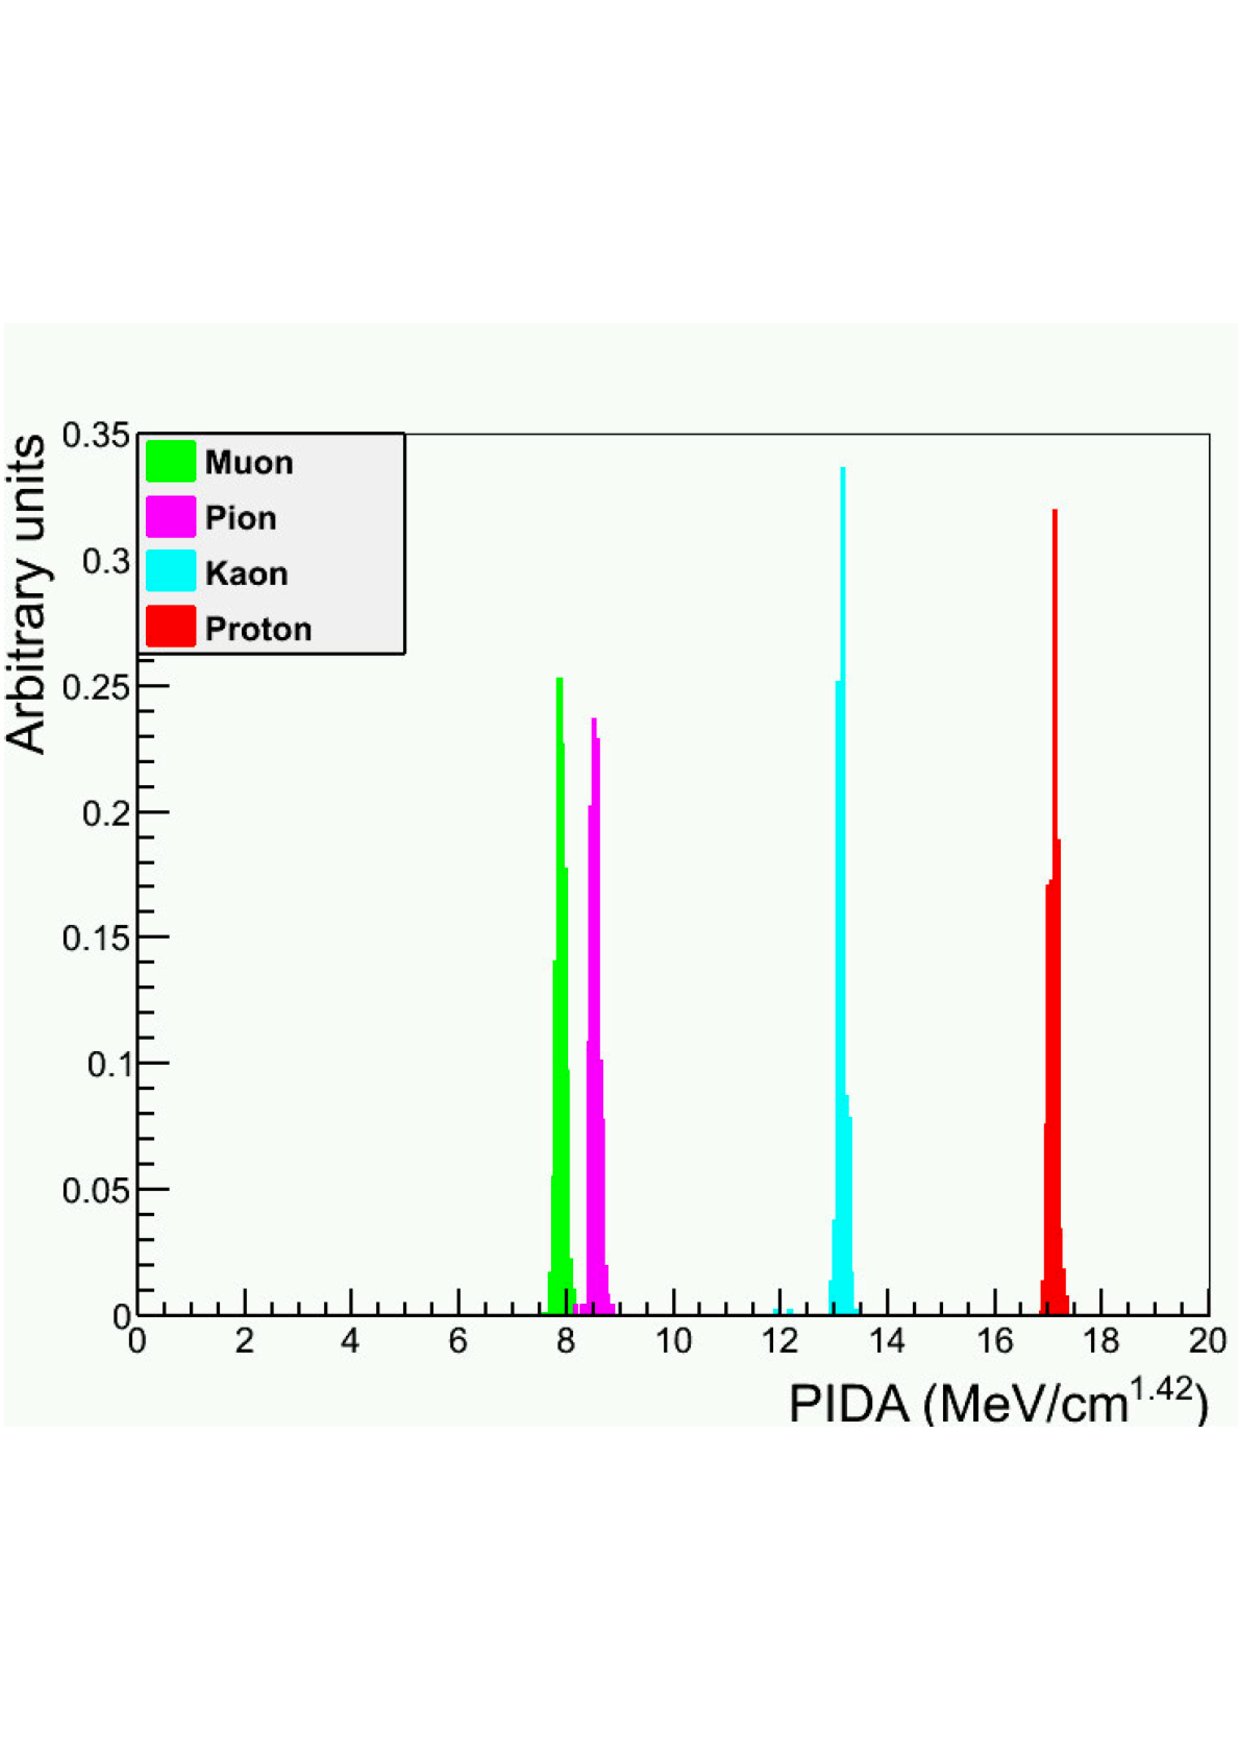
\includegraphics[width=\textwidth]{TruthPIDA}
    \caption{Distribution of PIDA values for different particle masses.}
    \label{fig:PIDA_MC}
  \end{subfigure}
  \caption[Defining the PIDA metric for particle identification.]
          {Defining the PIDA metric for particle identification and testing it on a Monte Carlo sample using truth information.}
  \label{fig:PIDAPlots}
\end{figure}

From Figure~\ref{fig:PIDAPlots} it can be seen that the most distinct PIDA distributions are that of muons and protons, these are also two of the most common particle types in cosmic rays. For these reasons particle identification using the PIDA variable will be attempted on simulations of the 35 ton. As outlined in Sections~\ref{sec:SimInteractionTimes} and ~\ref{sec:MCCalib} in order to do this the interaction times of particles have to be well known and the calibration constants must be tuned so as to ensure that the effects of recombination are properly accounted for. It is also useful to use the information found in Section~\ref{sec:SimRecoEffic} about the efficiency with which tracks are reconstructed. In this regard it is useful to produce additional figures showing the reconstruction efficiencies of protons in the CRY sample, these are shown in Figure~\ref{fig:Prot_Effic}.\\

\begin{figure}[h!]
  \centering
  \begin{subfigure}{.45\textwidth}
        \centering
        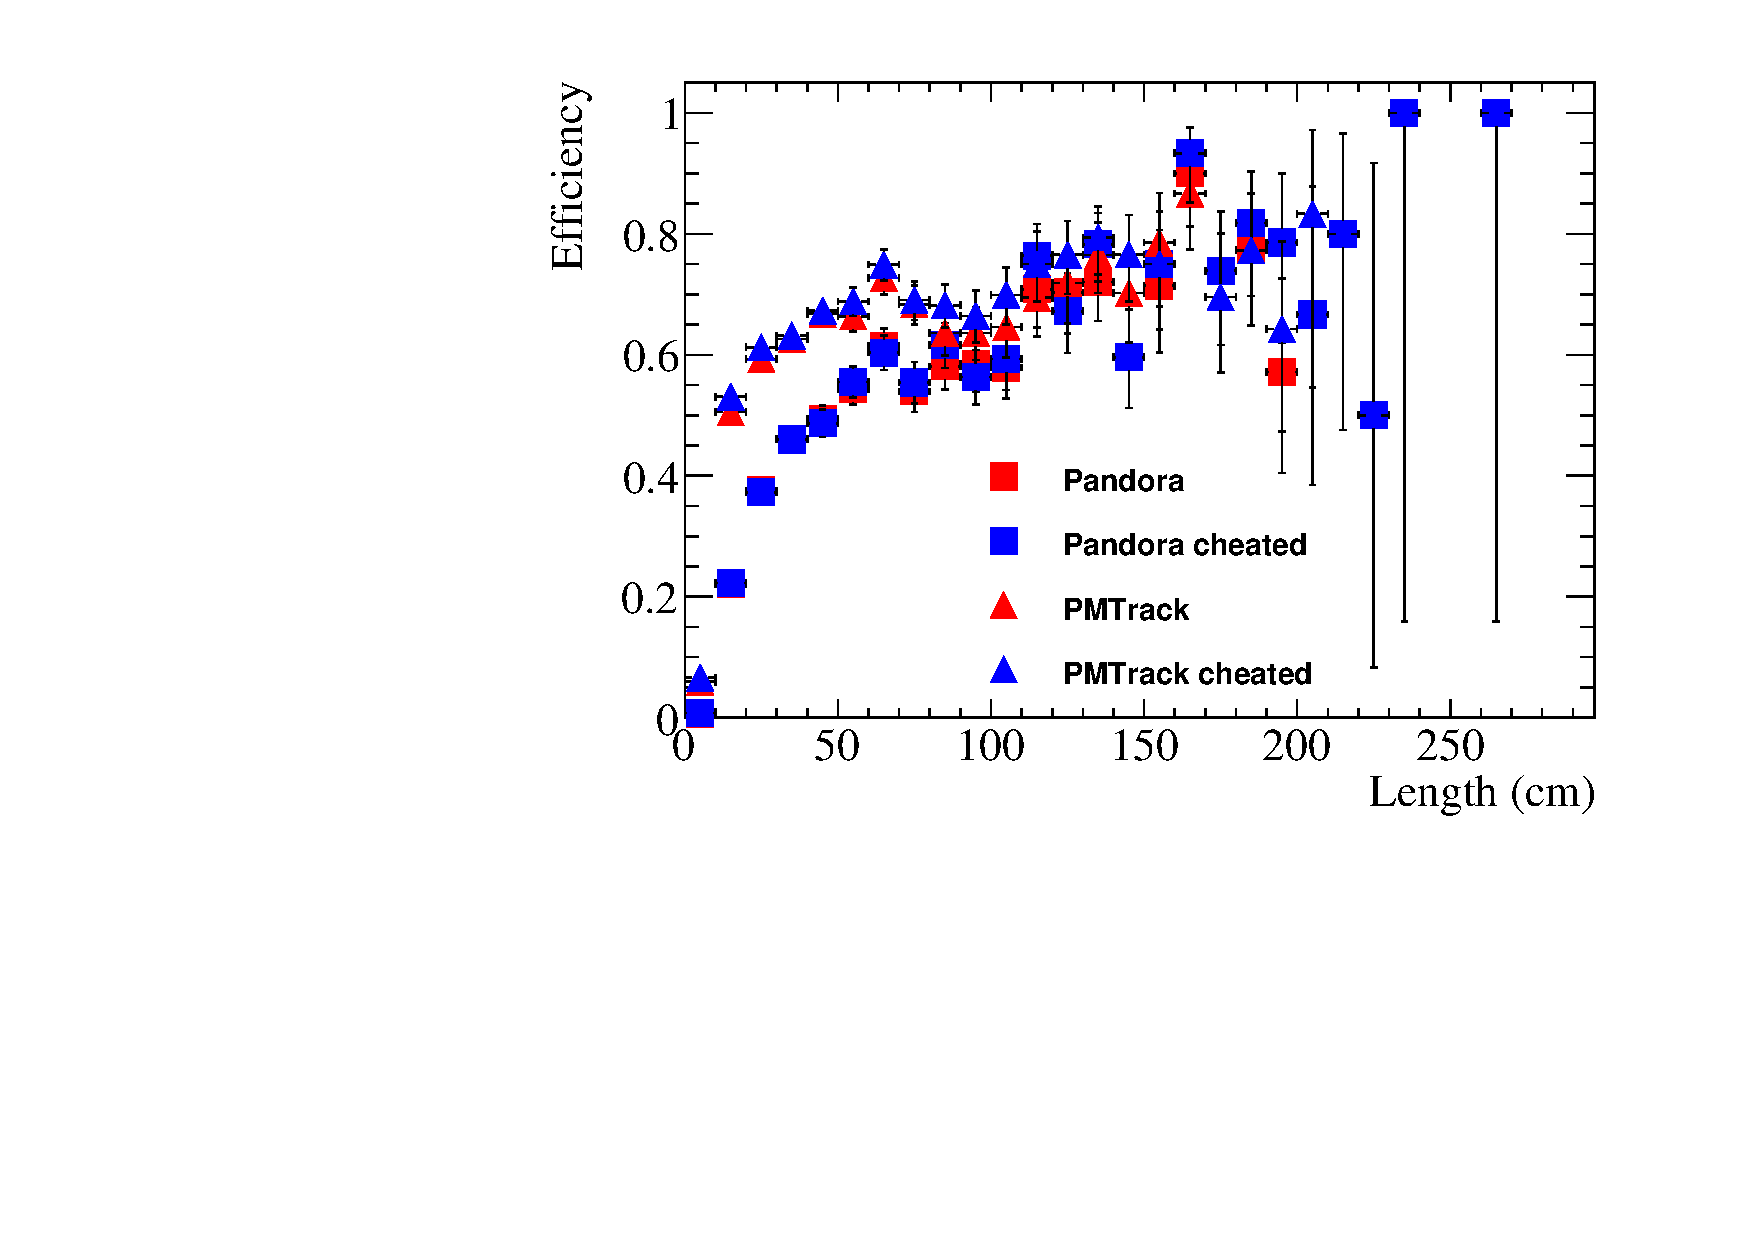
\includegraphics[width=\textwidth]{Effic_ProtonEnrich_500V_Proton_Length}
        \caption{The reconstruction efficiency as a function of Monte Carlo truth track length.}
        \label{fig:Prot_Effic_Len}
  \end{subfigure}
  \hspace{0.08\textwidth}
  \begin{subfigure}{.45\textwidth}
        \centering
        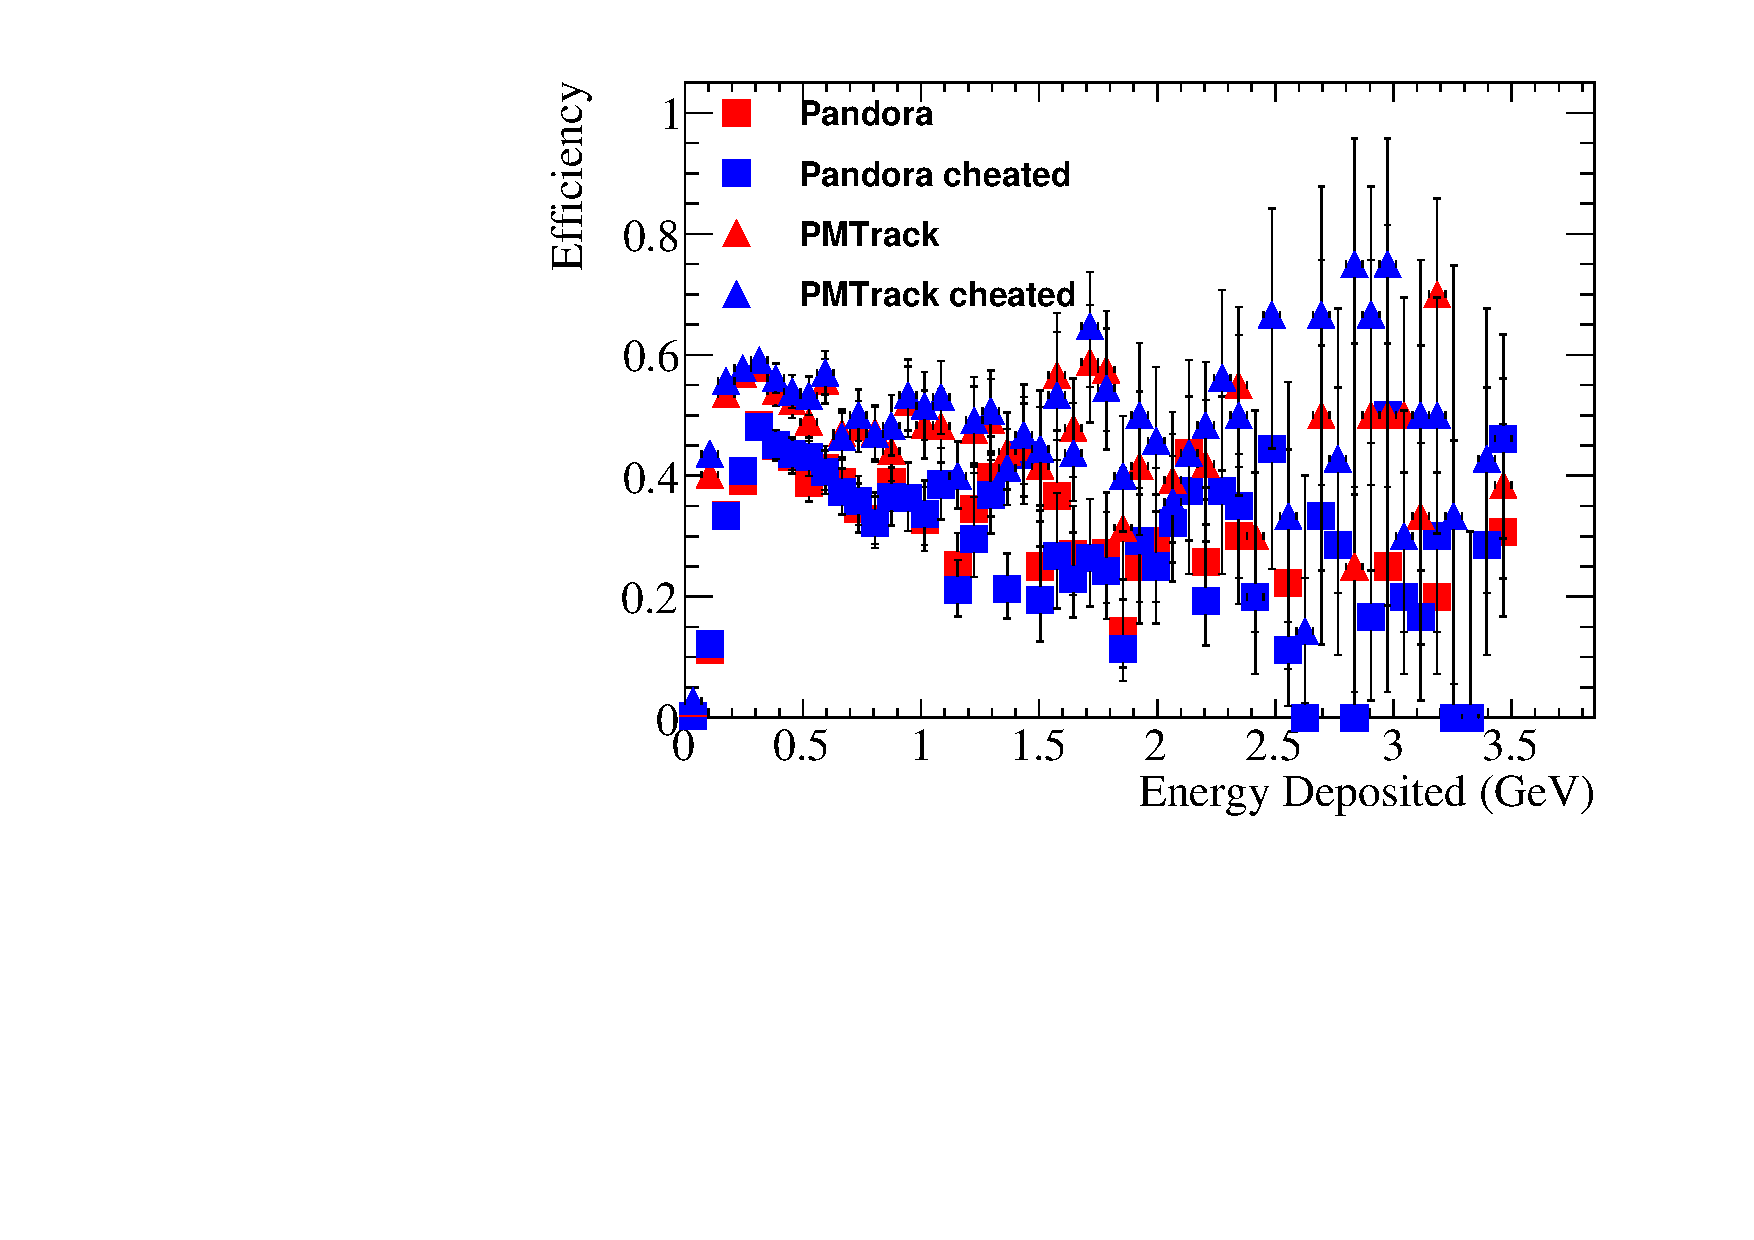
\includegraphics[width=\textwidth]{Effic_ProtonEnrich_500V_Proton_EnDepos}
        \caption{The reconstruction efficiency as a function of Monte Carlo truth deposited energy.}
        \label{fig:Prot_Effic_EnDepos}
  \end{subfigure}
  \begin{subfigure}{.45\textwidth}
        \centering
        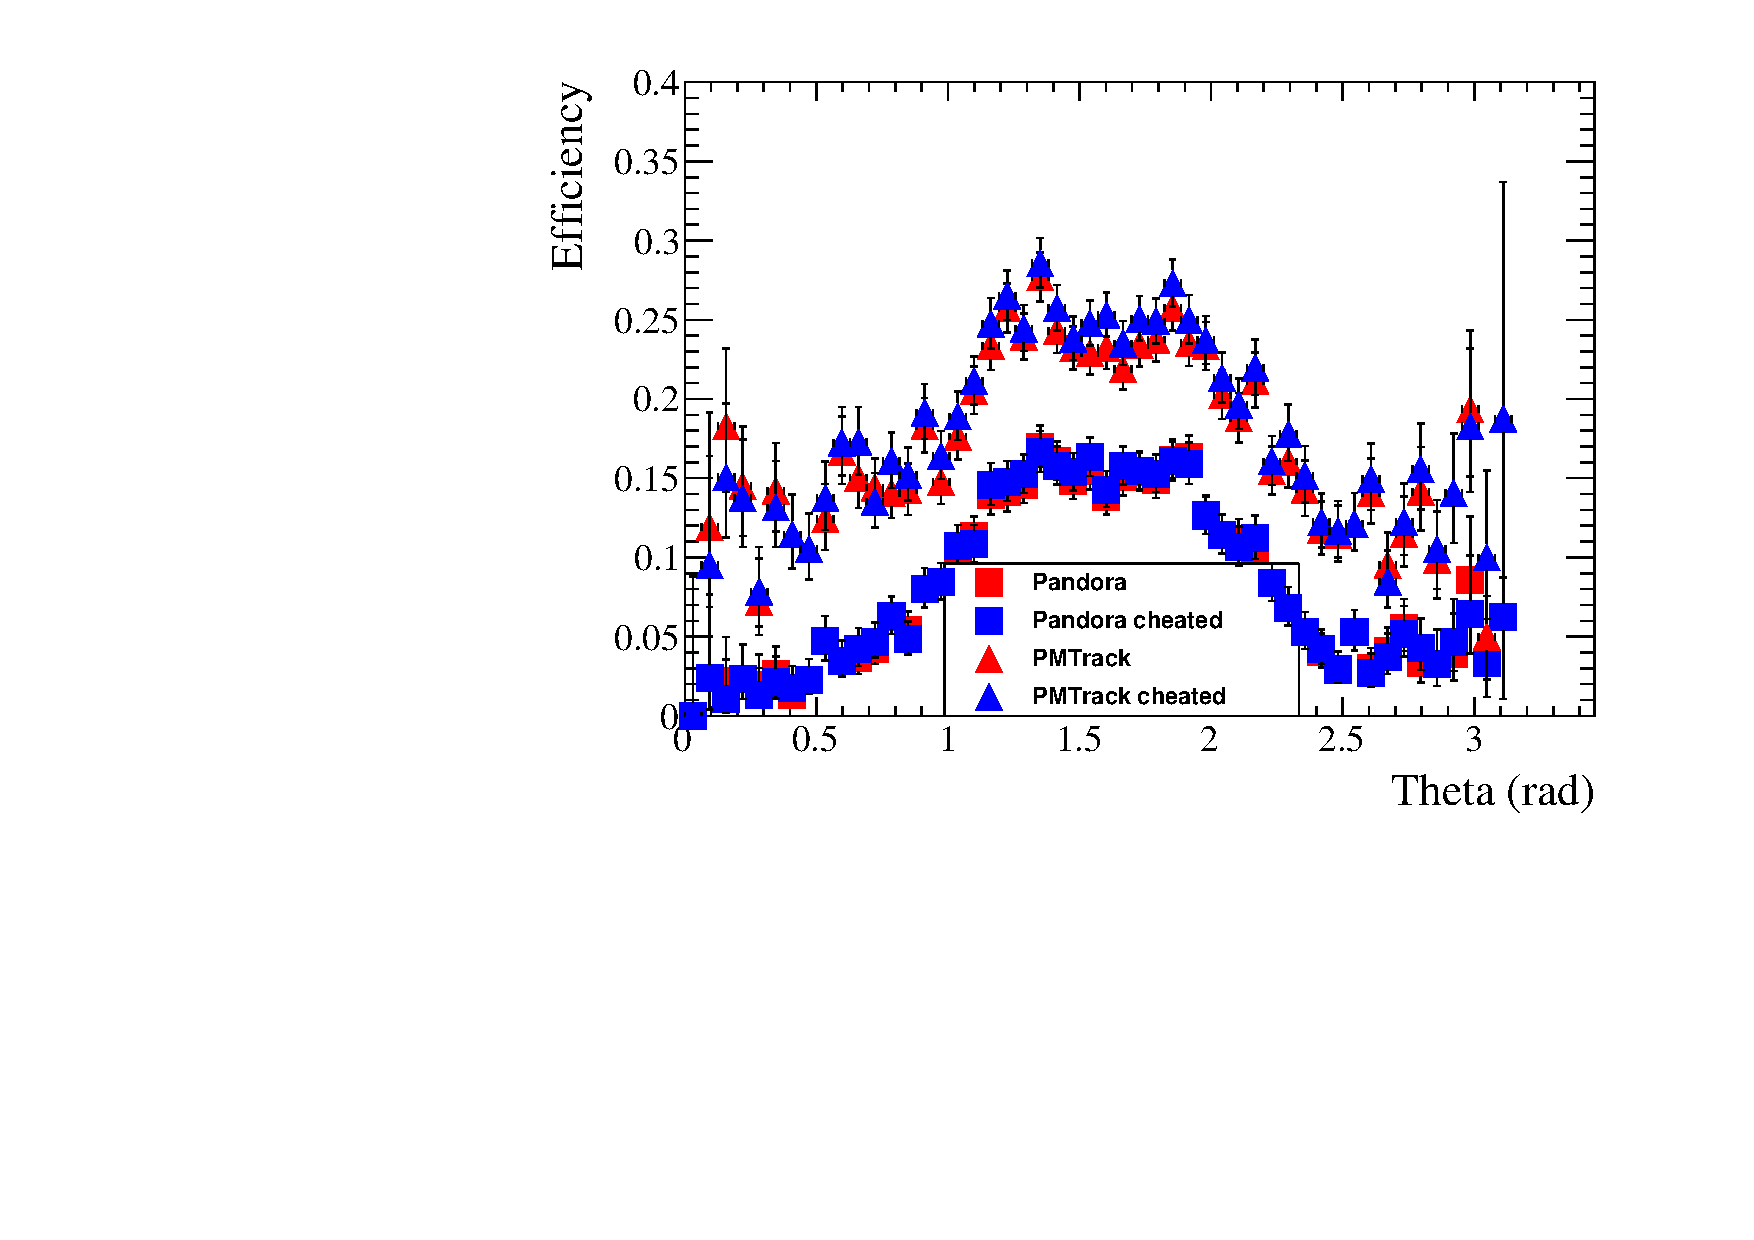
\includegraphics[width=\textwidth]{Effic_ProtonEnrich_500V_Proton_Theta}
        \caption{The reconstruction efficiency as a function of Monte Carlo truth track angle in theta.}
        \label{fig:Prot_Effic_Theta}
  \end{subfigure}
  \hspace{0.08\textwidth}
  \begin{subfigure}{.45\textwidth}
        \centering
        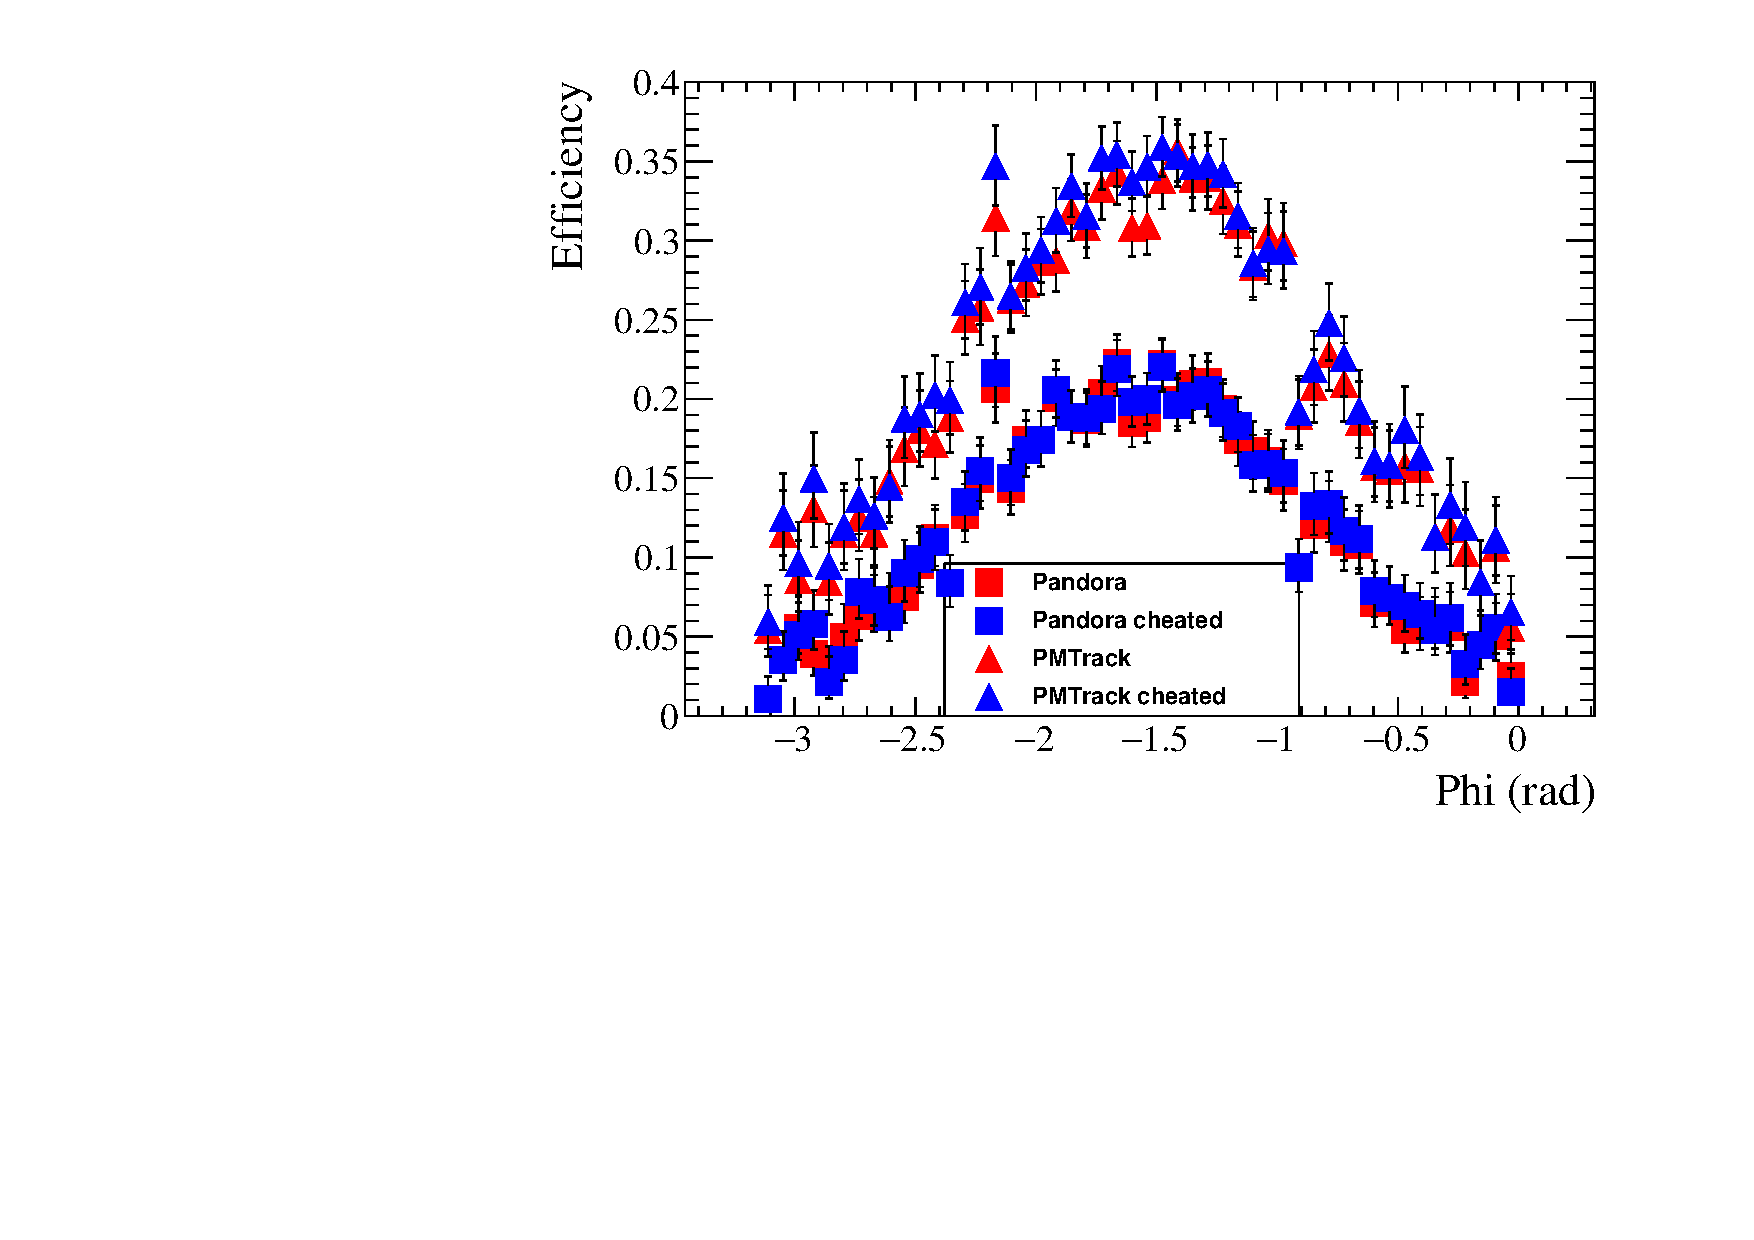
\includegraphics[width=\textwidth]{Effic_ProtonEnrich_500V_Proton_Phi}
        \caption{The reconstruction efficiency as a function of Monte Carlo truth track angle in phi.}
        \label{fig:Prot_Effic_Phi}
  \end{subfigure}
  \begin{subfigure}{.45\textwidth}
        \centering
        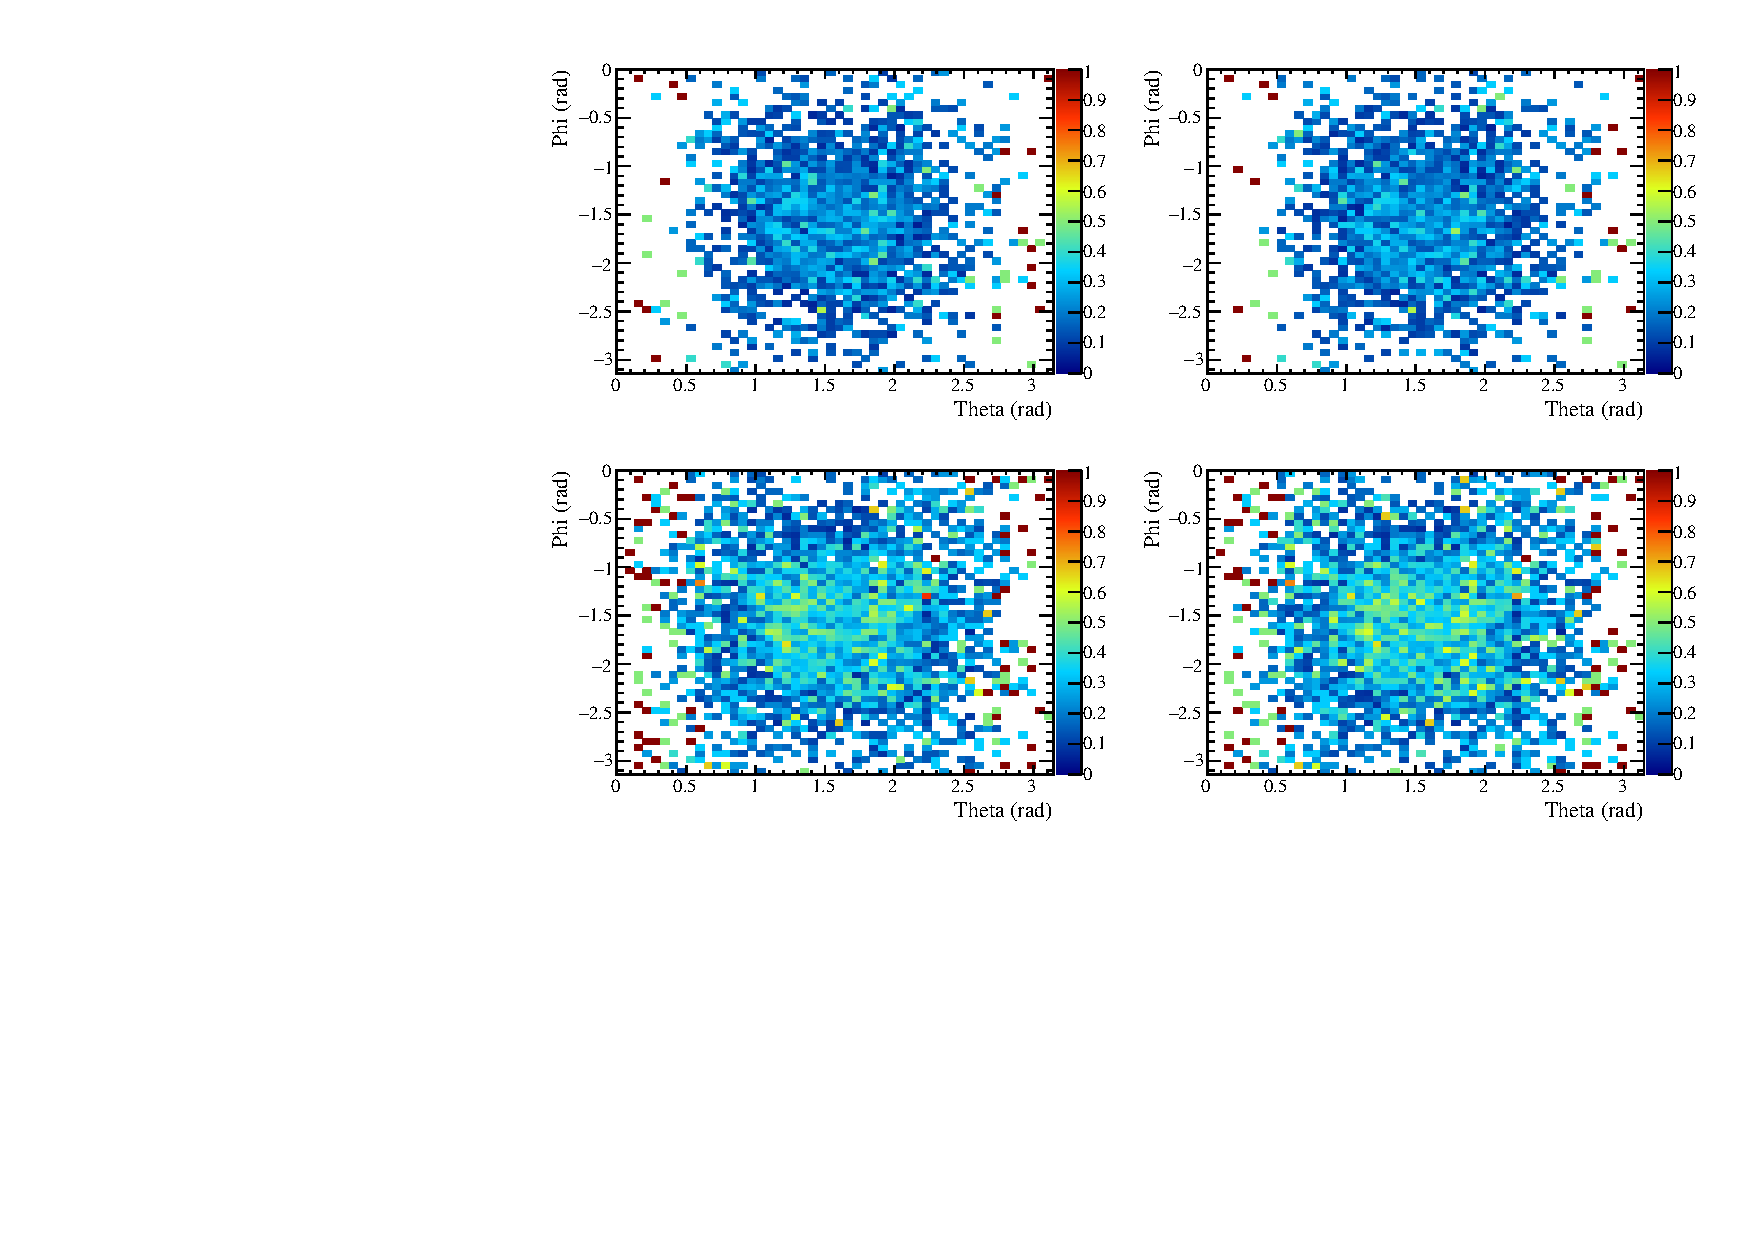
\includegraphics[width=\textwidth]{Effic_ProtonEnrich_500V_Proton_PhiTheta}
        \caption{The reconstruction efficiency as a function of Monte Carlo truth track angle in theta and phi.}
        \label{fig:Prot_Effic_PhiTheta}
  \end{subfigure}
  \caption[The reconstruction efficiencies for protons in a sample generated using CRY.]
          {The reconstruction efficiencies for protons in a sample generated using CRY. The efficiencies are shown for non-cheated reconstruction (red blocks) and cheated reconstruction (blue blocks) for both Pandora (square blocks) and PMTrack (triangle blocks).}
  \label{fig:Prot_Effic}
\end{figure}

Figure~\ref{fig:Prot_Effic} shows that the average reconstruction efficiency for PMTrack is higher than that for Pandora when considering protons, as the efficiency for the former is roughly 10\% higher for all angles as shown in Figure~\ref{fig:Prot_Effic_Theta}, though it is much lower than the overall efficiency seen in Figure~\ref{fig:SimEffic_Theta_CRY}. From Figure~\ref{fig:Prot_Effic_Len} it is evident that the efficiency for protons with track lengths of more than 10 cm is similar to that of the overall efficiency for the CRY sample, but the efficiency for the shortest tracks is significantly lower than that of the whole CRY sample. A review of the true path lengths of the simulated particles shows that 60\% of the protons have path lengths of less than 1 cm and that none of these particles were reconstructed, it is this large number of very short particles which causes the overall reconstruction to be relatively low. When a minimum path length of 1 cm (10 cm) is required the reconstruction efficiency rises to 37\% (58\%), so when the shortest tracks are not counted the reconstruction performs reasonably well. \\

It is also useful to produce samples where the primary particle is a single muon or proton located in the active volume of the detector. This allows for a sample of isolated tracks to be made upon which the capabilities of the PIDA metric can be tested. It also allows the reconstruction efficiency to be found for particles in isolation. The properties of the generated particles are illustrated below in Table~\ref{tab:IsolProp}. The values of the simulated quantities were found by changing the given parameters by an amount taken from a random sampling of a Gaussian distribution of width equal to the error listed. These simulation parameters were chosen to produce samples which would contain both exiting and stopping particles whilst generating the particles in the LAr would ensure that there should always be a reconstructable track in the detector. \\

The reconstruction efficiencies when using the PMTrack reconstruction method are shown for the simulated particles in Figure~\ref{fig:Isol_Effic}. It should be noted that truth particles with track lengths of less than 1 cm have been excluded from these plots which is why the angular reconstruction efficiencies for protons in Figures~\ref{fig:Isol_Effic_Theta} and~\ref{fig:Isol_Effic_Phi}, are higher than those seen in Figures~\ref{fig:Prot_Effic_Theta} and~\ref{fig:Prot_Effic_Phi}. This was done as due to how the initial momenta and positions are sampled many of the primary simulated particles may travel very short distances that are contained in spaces between TPCs and including these particles would artificially reduce the efficiency presented. After discounting these very short particles the efficiencies generally follow similar patterns observed in the earlier efficiency plots, though there is a decrease in efficiencies for the longest track lengths which is not observed in other samples. This is attributed to the initial positions for the particles being within the detector volume, as this means that any particle travelling over 100 cm would have a very peculiar trajectory as the edge of the detector should never be more than 100 cm away from the starting position. The only exception to this is if a particle travelled along the x axis to the other end of the detector, which as discussed earlier is a very problematic orientation to reconstruct as all of the charge would be deposited over a large range of time on very few collection plane wires. \\

\begin{table}
\caption{The properties of initial particles simulated in the muon and proton samples.}
\centering
\label{tab:IsolProp}
\begin{tabular}{l c c}
\toprule
{} & {Muon properties} & {Proton properties} \\ 
\midrule
Initial position (cm)              & (100 $\pm$ 50, 0 $\pm$ 30, 80 $\pm$ 20) & (100 $\pm$ 50, 0 $\pm$ 30, 80 $\pm$ 20)  \\

Initial momentum (GeV)            & 0.3 $\pm$ 0.1 & 0.8 $\pm$ 0.5 \\

Initial $\theta_{XZ}$ $(^{\circ})$ &   0 $\pm$ 180 &   0 $\pm$ 180 \\

Initial $\theta_{YZ}$ $(^{\circ})$ & -45 $\pm$ 45  & -45 $\pm$ 45  \\
\bottomrule
\end{tabular}
\end{table}

\begin{figure}[h!]
  \centering
  \begin{subfigure}{.45\textwidth}
        \centering
        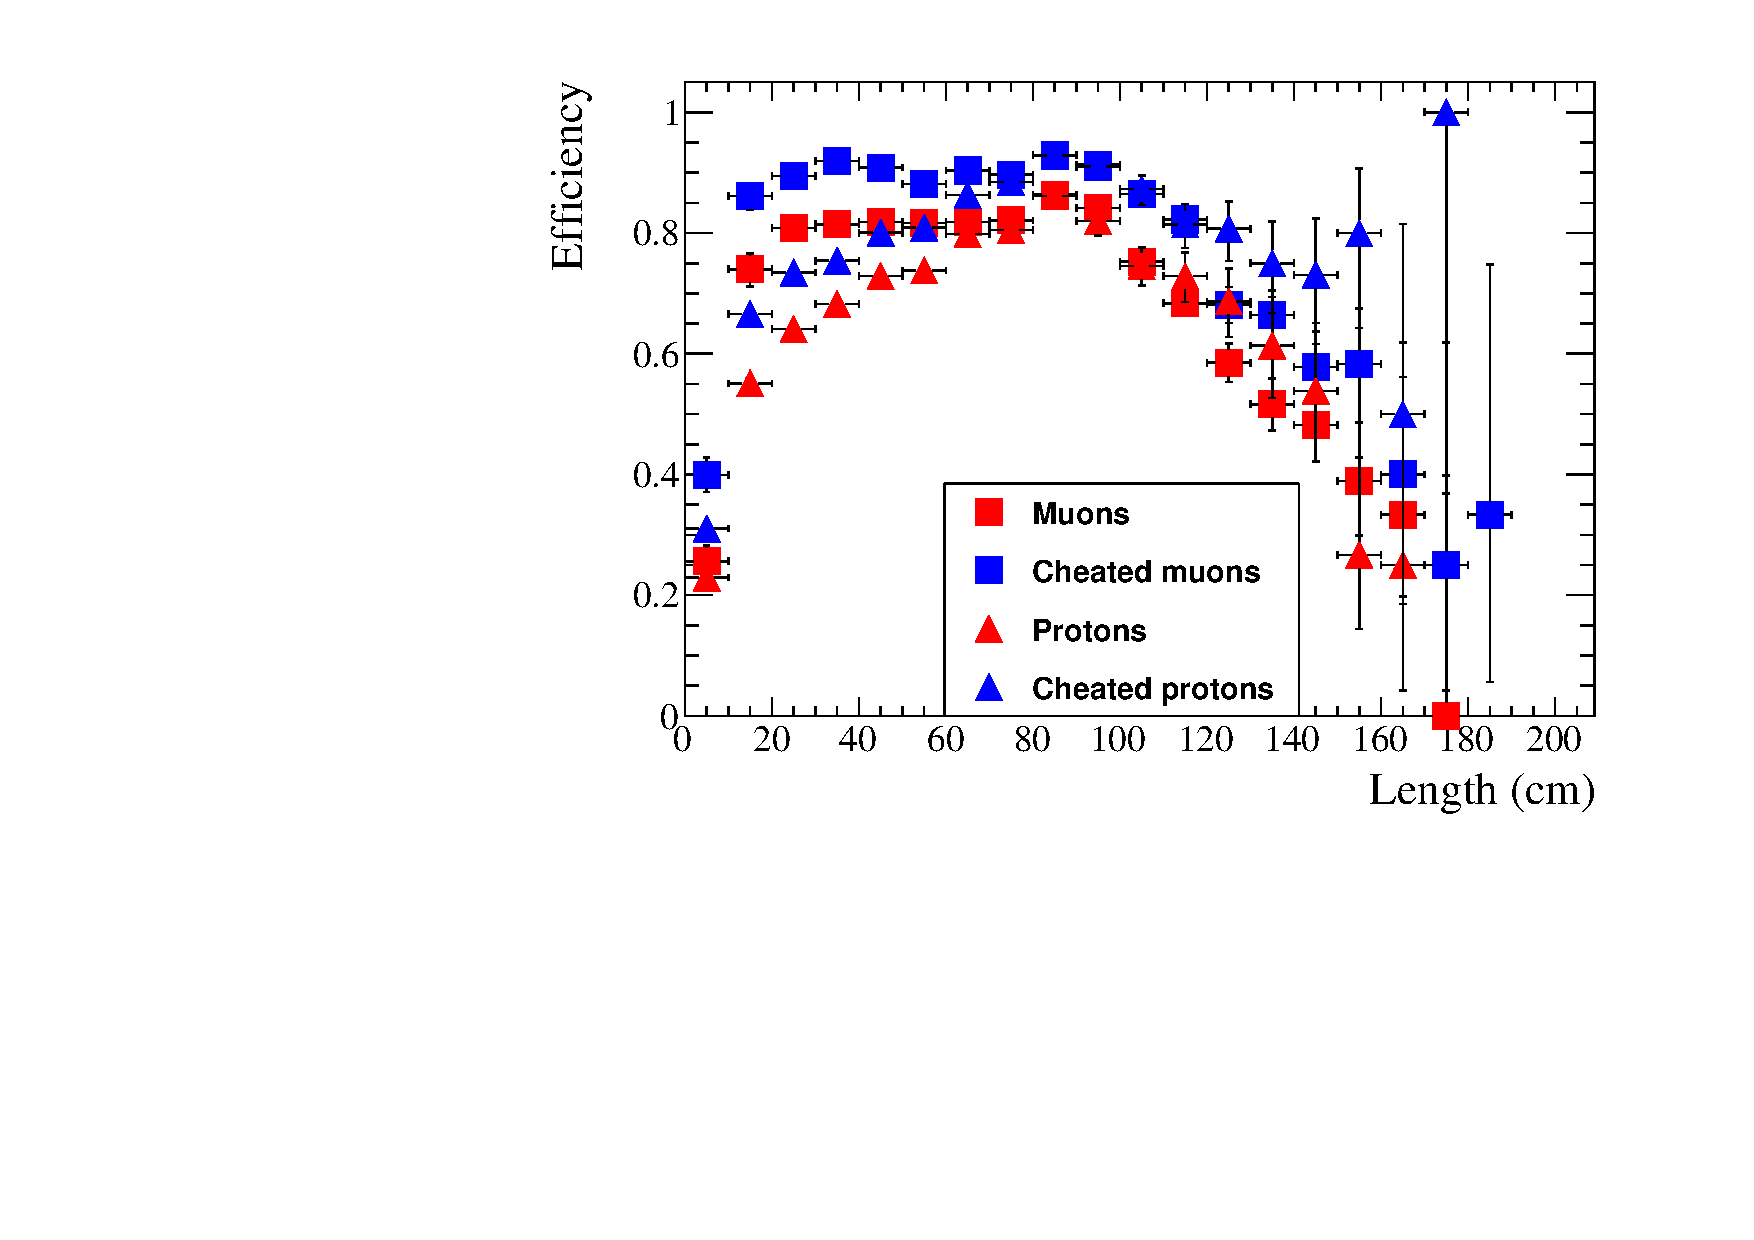
\includegraphics[width=\textwidth]{Effic_SingSamps_Length}
        \caption{The reconstruction efficiency as a function of Monte Carlo truth track length.}
        \label{fig:Isol_Effic_Len}
  \end{subfigure}
  \hspace{0.08\textwidth}
  \begin{subfigure}{.45\textwidth}
        \centering
        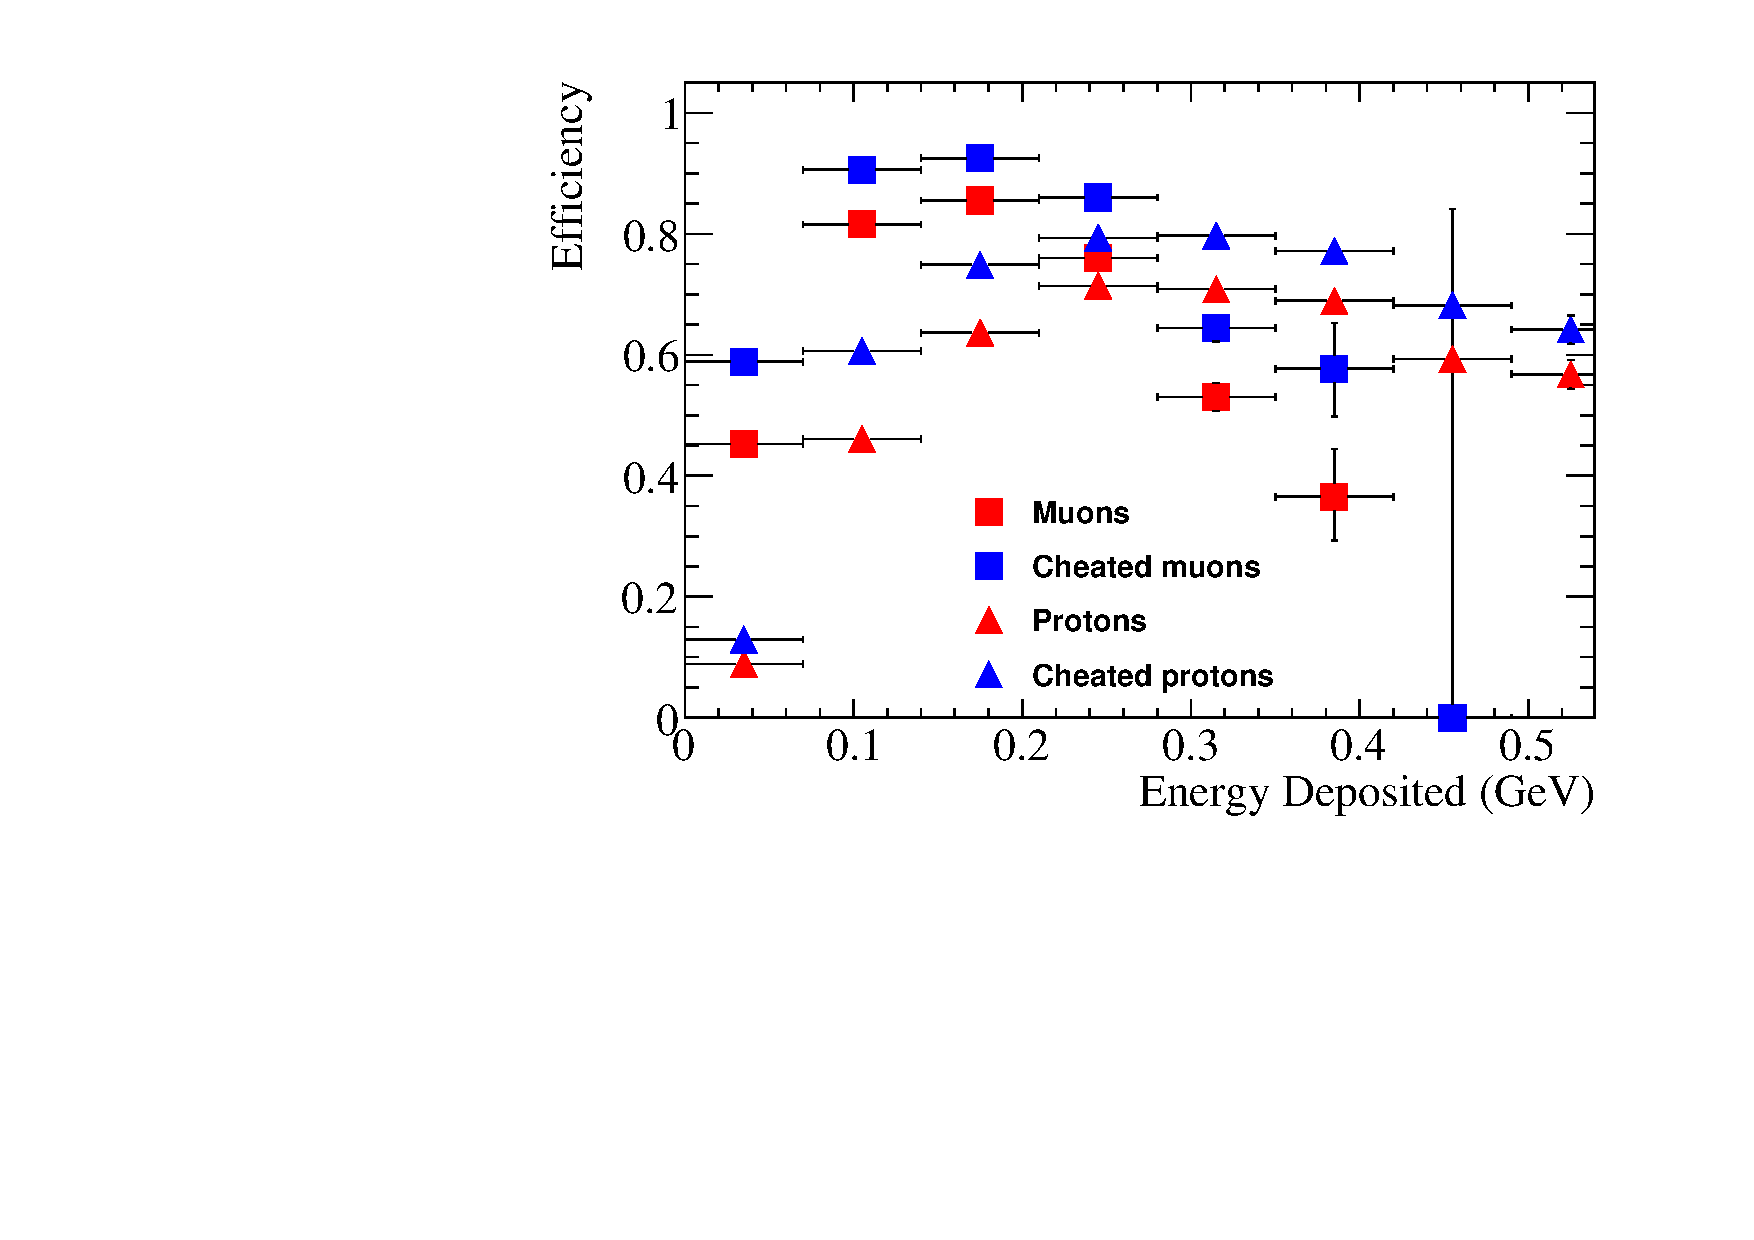
\includegraphics[width=\textwidth]{Effic_SingSamps_EnDepos}
        \caption{The reconstruction efficiency as a function of Monte Carlo truth deposited energy.}
        \label{fig:Isol_Effic_EnDepos}
  \end{subfigure}
  \begin{subfigure}{.45\textwidth}
        \centering
        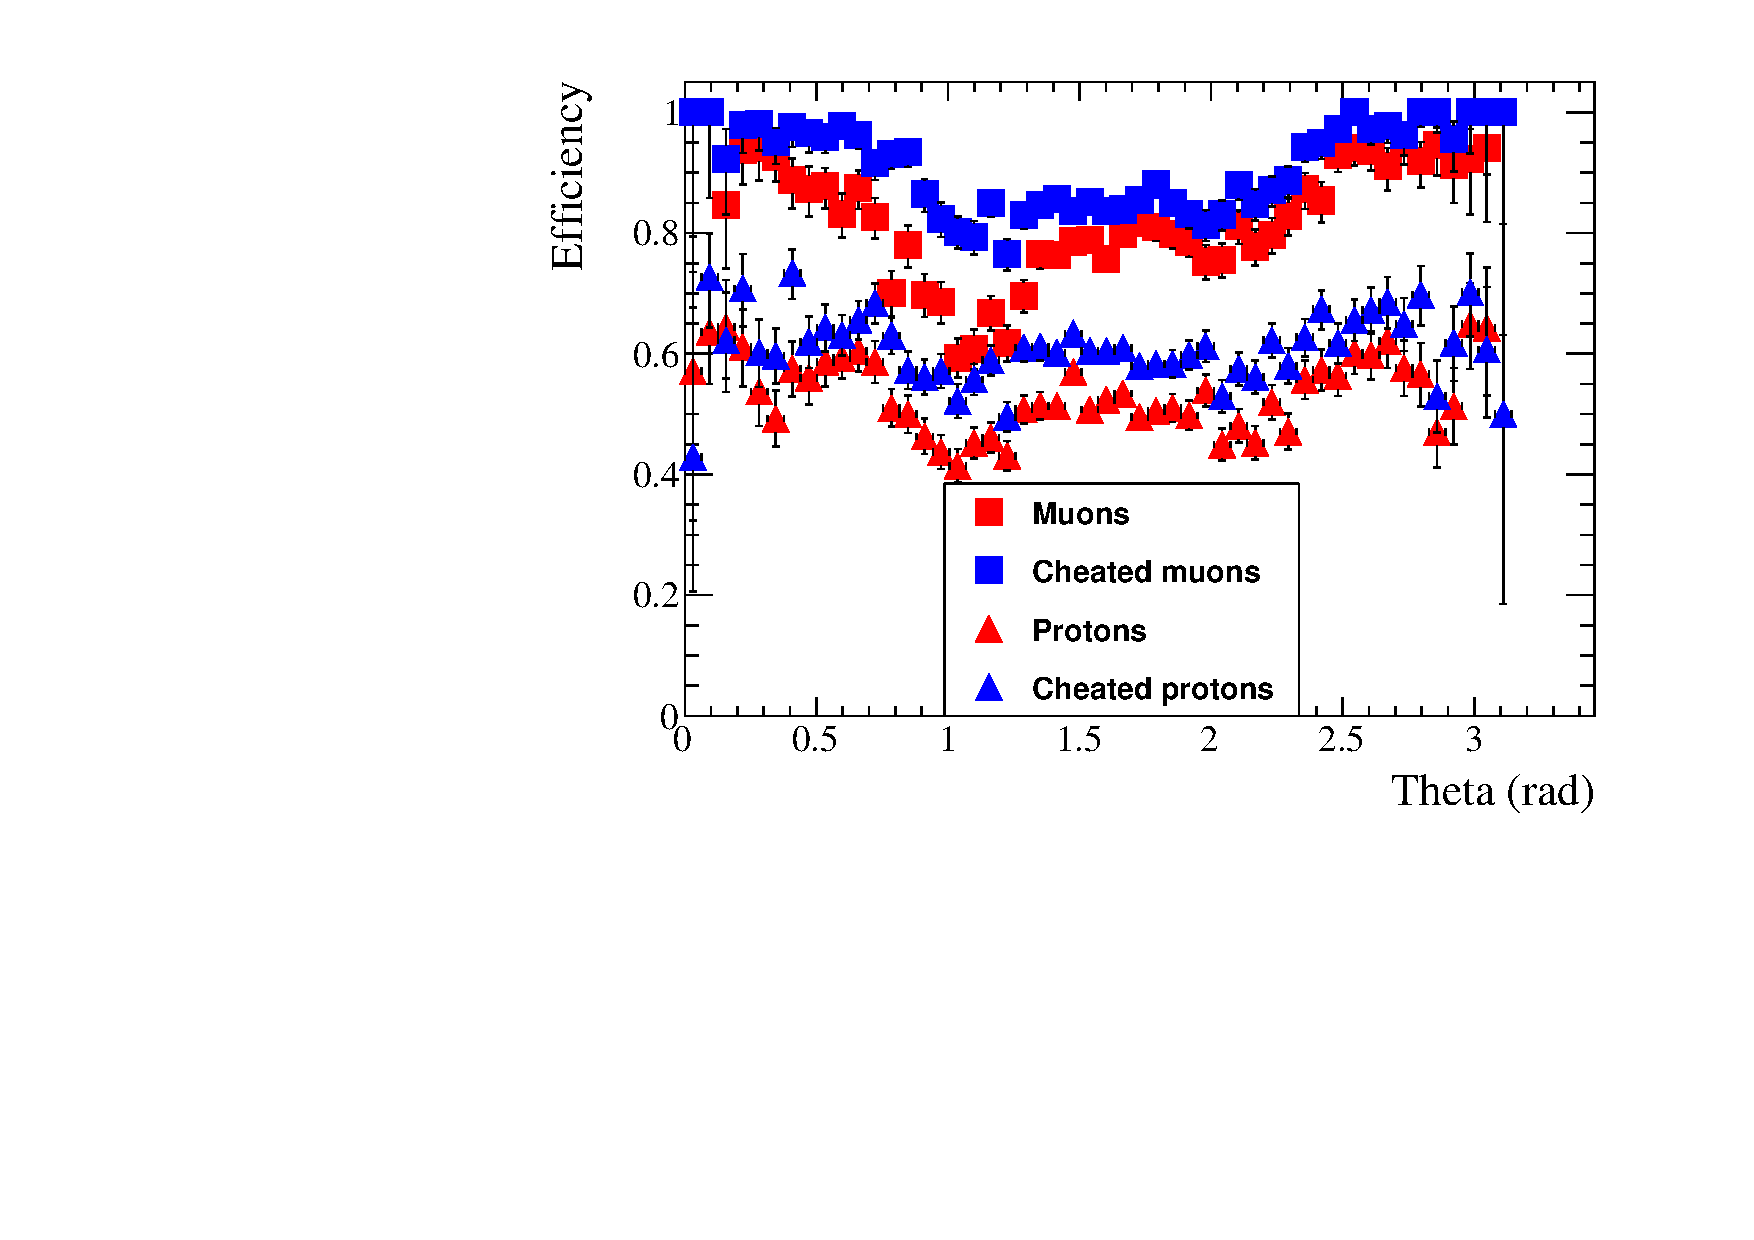
\includegraphics[width=\textwidth]{Effic_SingSamps_Theta}
        \caption{The reconstruction efficiency as a function of Monte Carlo truth track angle in theta.}
        \label{fig:Isol_Effic_Theta}
  \end{subfigure}
  \hspace{0.08\textwidth}
  \begin{subfigure}{.45\textwidth}
        \centering
        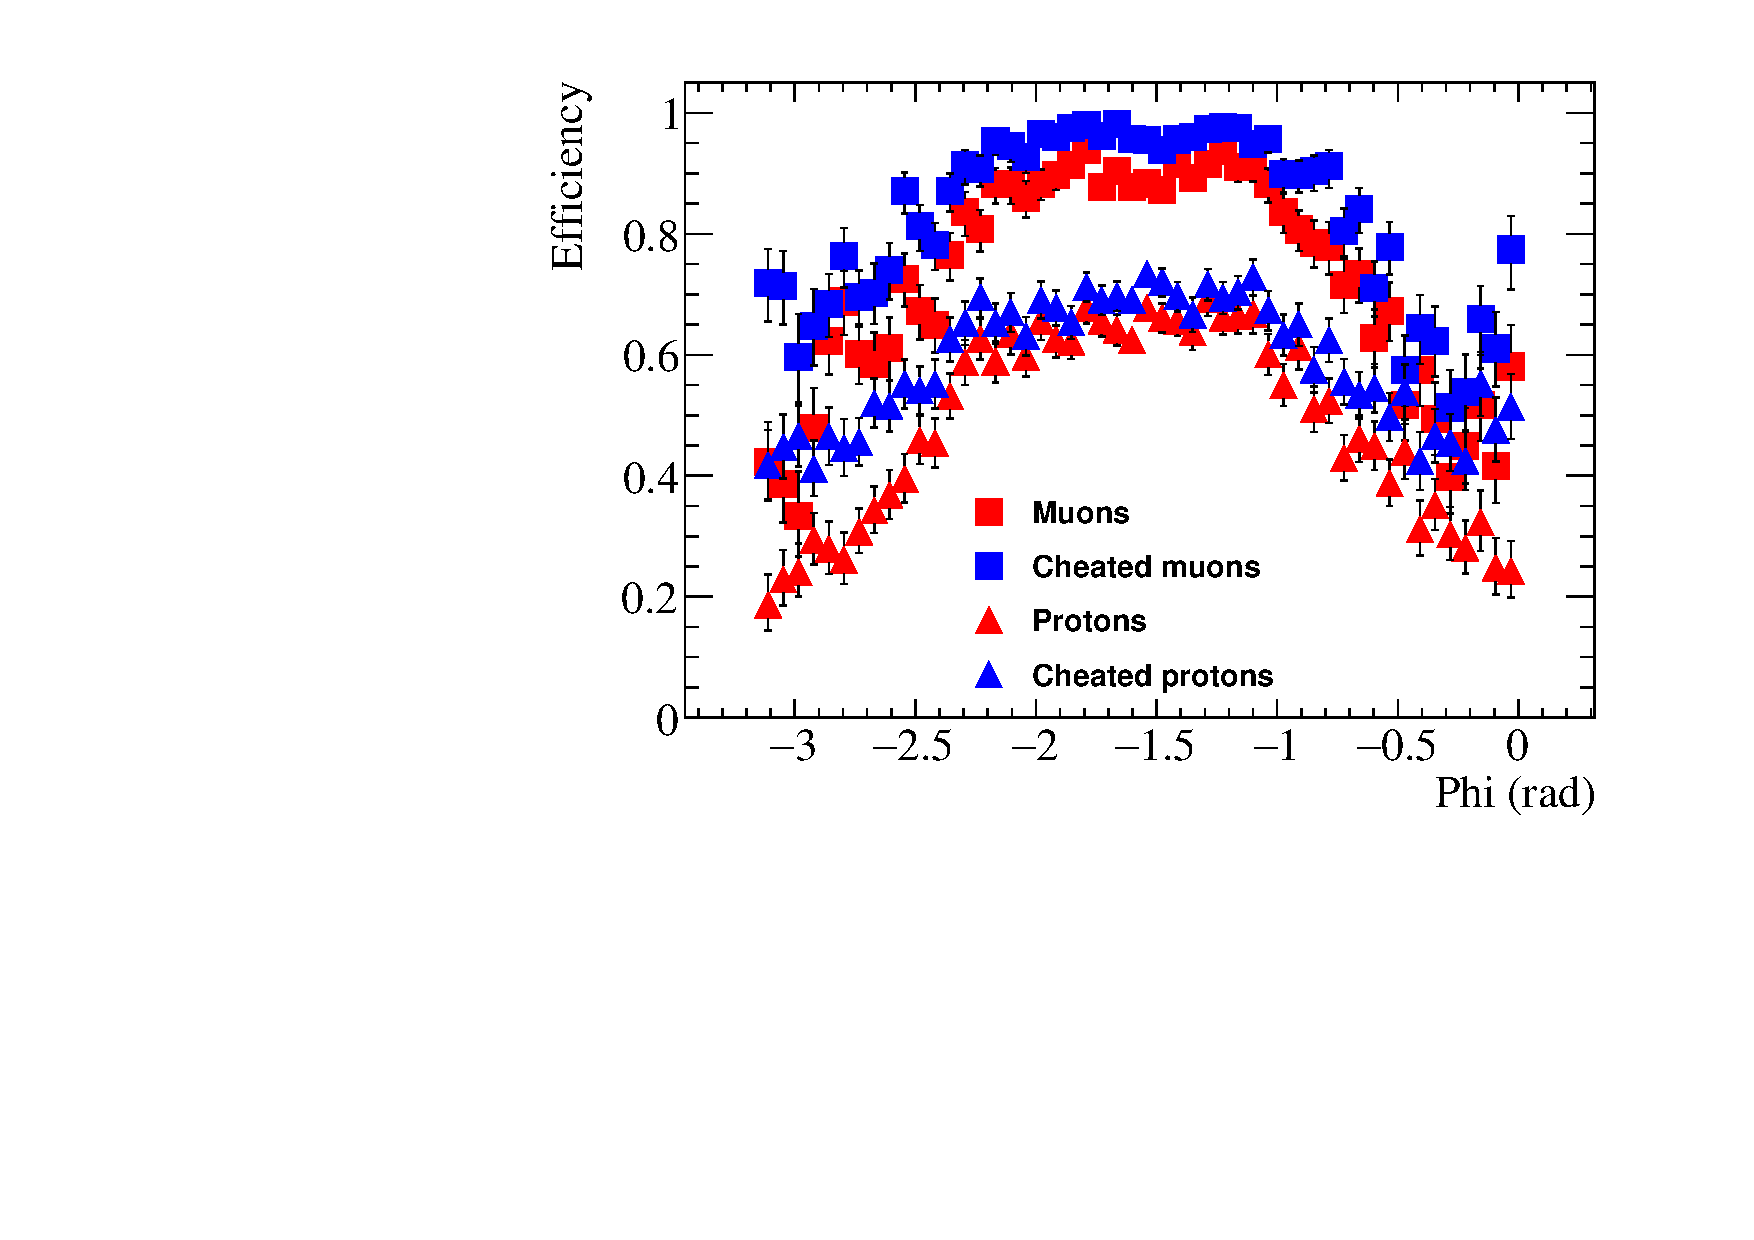
\includegraphics[width=\textwidth]{Effic_SingSamps_Phi}
        \caption{The reconstruction efficiency as a function of Monte Carlo truth track angle in phi.}
        \label{fig:Isol_Effic_Phi}
  \end{subfigure}
  \begin{subfigure}{.45\textwidth}
        \centering
        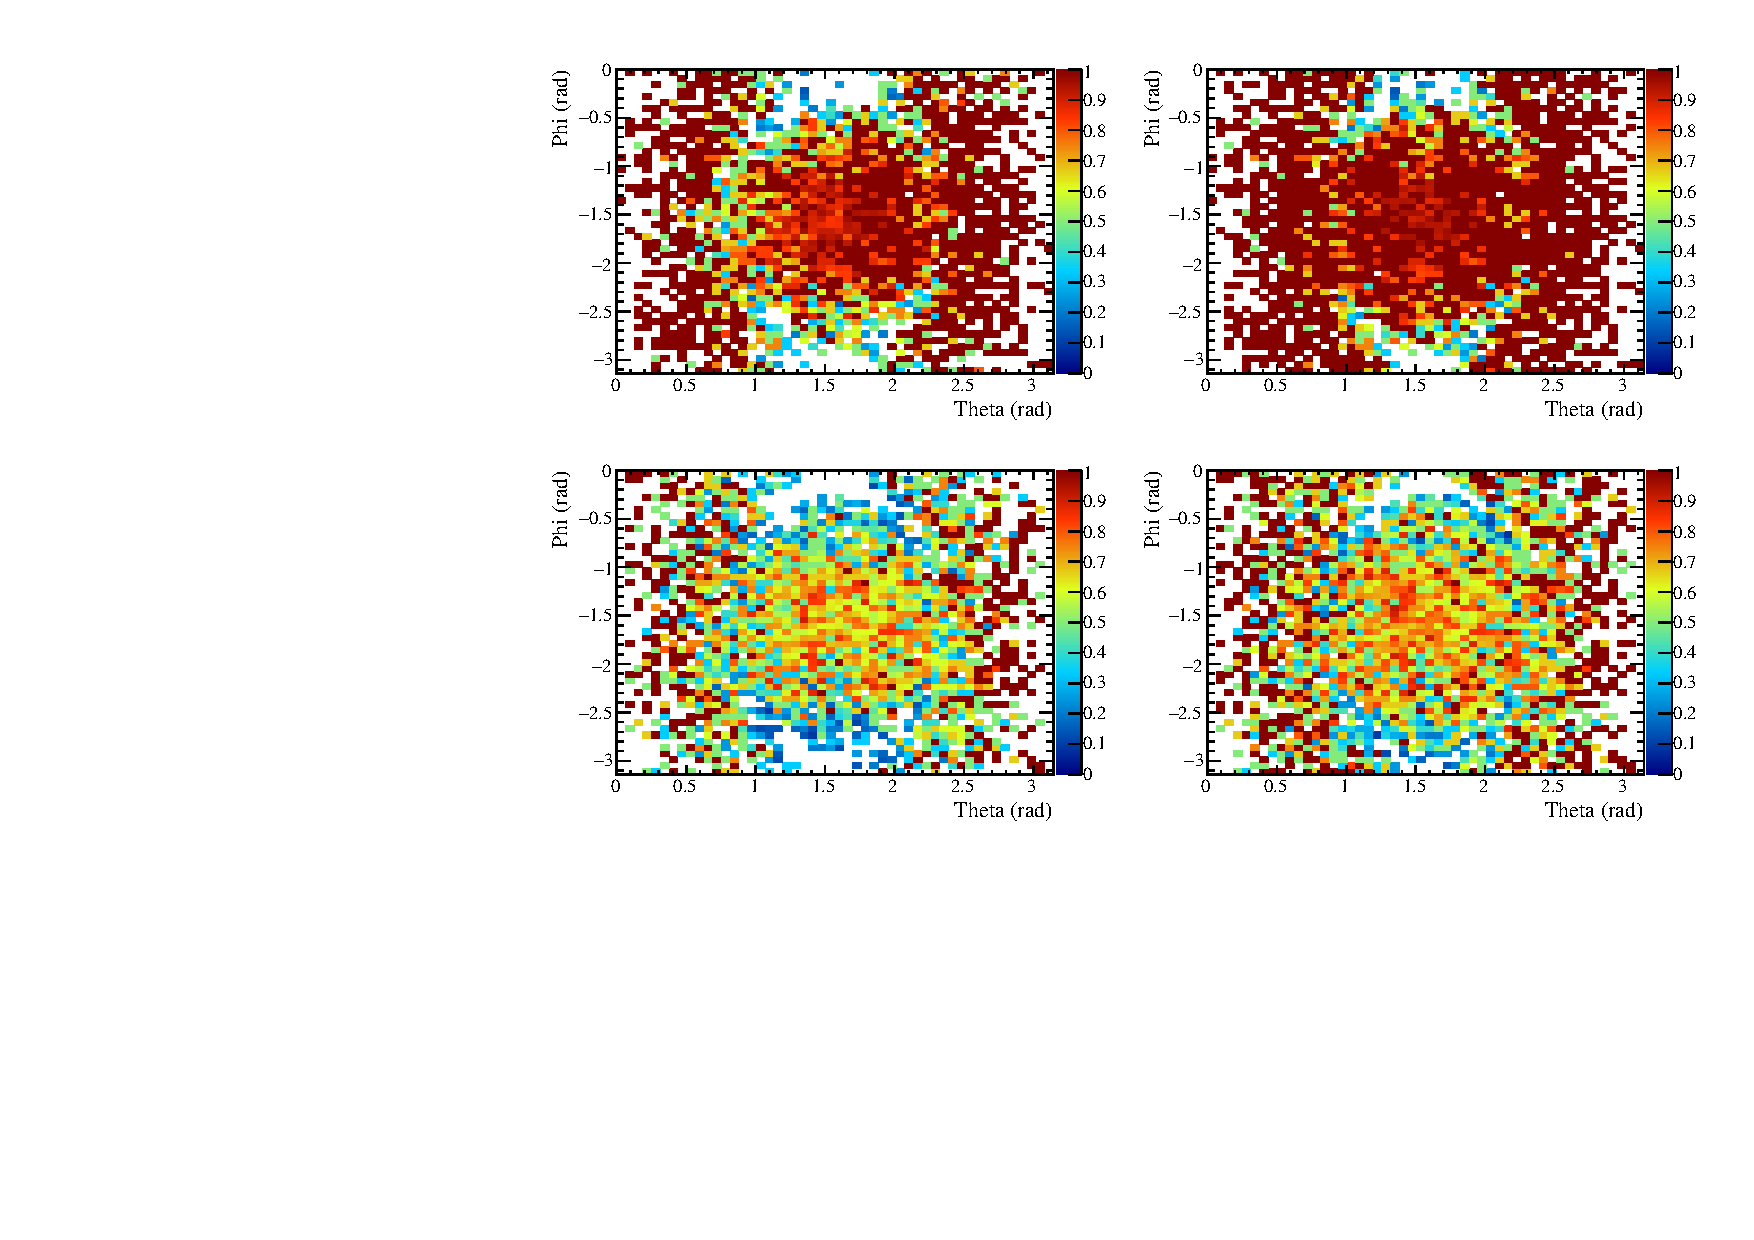
\includegraphics[width=\textwidth]{Effic_SingSamps_PhiTheta}
        \caption{The reconstruction efficiency as a function of Monte Carlo truth track angle in theta and phi.}
        \label{fig:Isol_Effic_PhiTheta}
  \end{subfigure}
  \caption[The reconstruction efficiencies for single muons and protons in the 35 ton.]
          {The reconstruction efficiencies for single muons and protons in the 35 ton. The efficiencies are shown for non-cheated reconstruction (red blocks) and cheated reconstruction (blue blocks) for both muons (square blocks) and protons (triangle blocks).}
  \label{fig:Isol_Effic}
\end{figure}

As the increase in $\frac{dE}{dx}$ is only visible when the particle stops in the detector it is necessary to remove exiting particles from the sample by applying a fiducial cut on the end point of the reconstructed track. It is important to only place this on the end point of the track, as one does not want to remove particles which enter the detector and then stop. When calorimetry is performed the end point of the track is determined using, among other metrics, the increase in $\frac{dE}{dx}$ and so the residual range of the track (a stored data member of the track object) should always refer to the distance to the end of the particles trajectory. For this study a fiducial cut of 5 cm is used, meaning that any track with hits within 5 cm of the edge of the detector volume is discarded and counted as an exiting particle. This should mean that very few tracks due to exiting particles are identified as stopping in the detector as it would require that a large section of the track would have to un-reconstructed. This will mean that some stopping particles are incorrectly assigned as exiting particles causing the identification efficiency to drop, but it is necessary to ensure that exiting particles are not included in the final distributions. A further cut that is applied is the requirement that there are a minimum of 5 continuous collection plane hits, this is to ensure that an adequate number of points are taken upon which to find an average value of PIDA for the track. Similar cuts are described in~\citep{PIDA_Paper}, and the resulting distributions of PIDA values for the single proton and muon samples are shown in Figure~\ref{fig:Isol_PIDA}. \\

\begin{figure}[h!]
  \centering
  \begin{subfigure}{.45\textwidth}
        \centering
        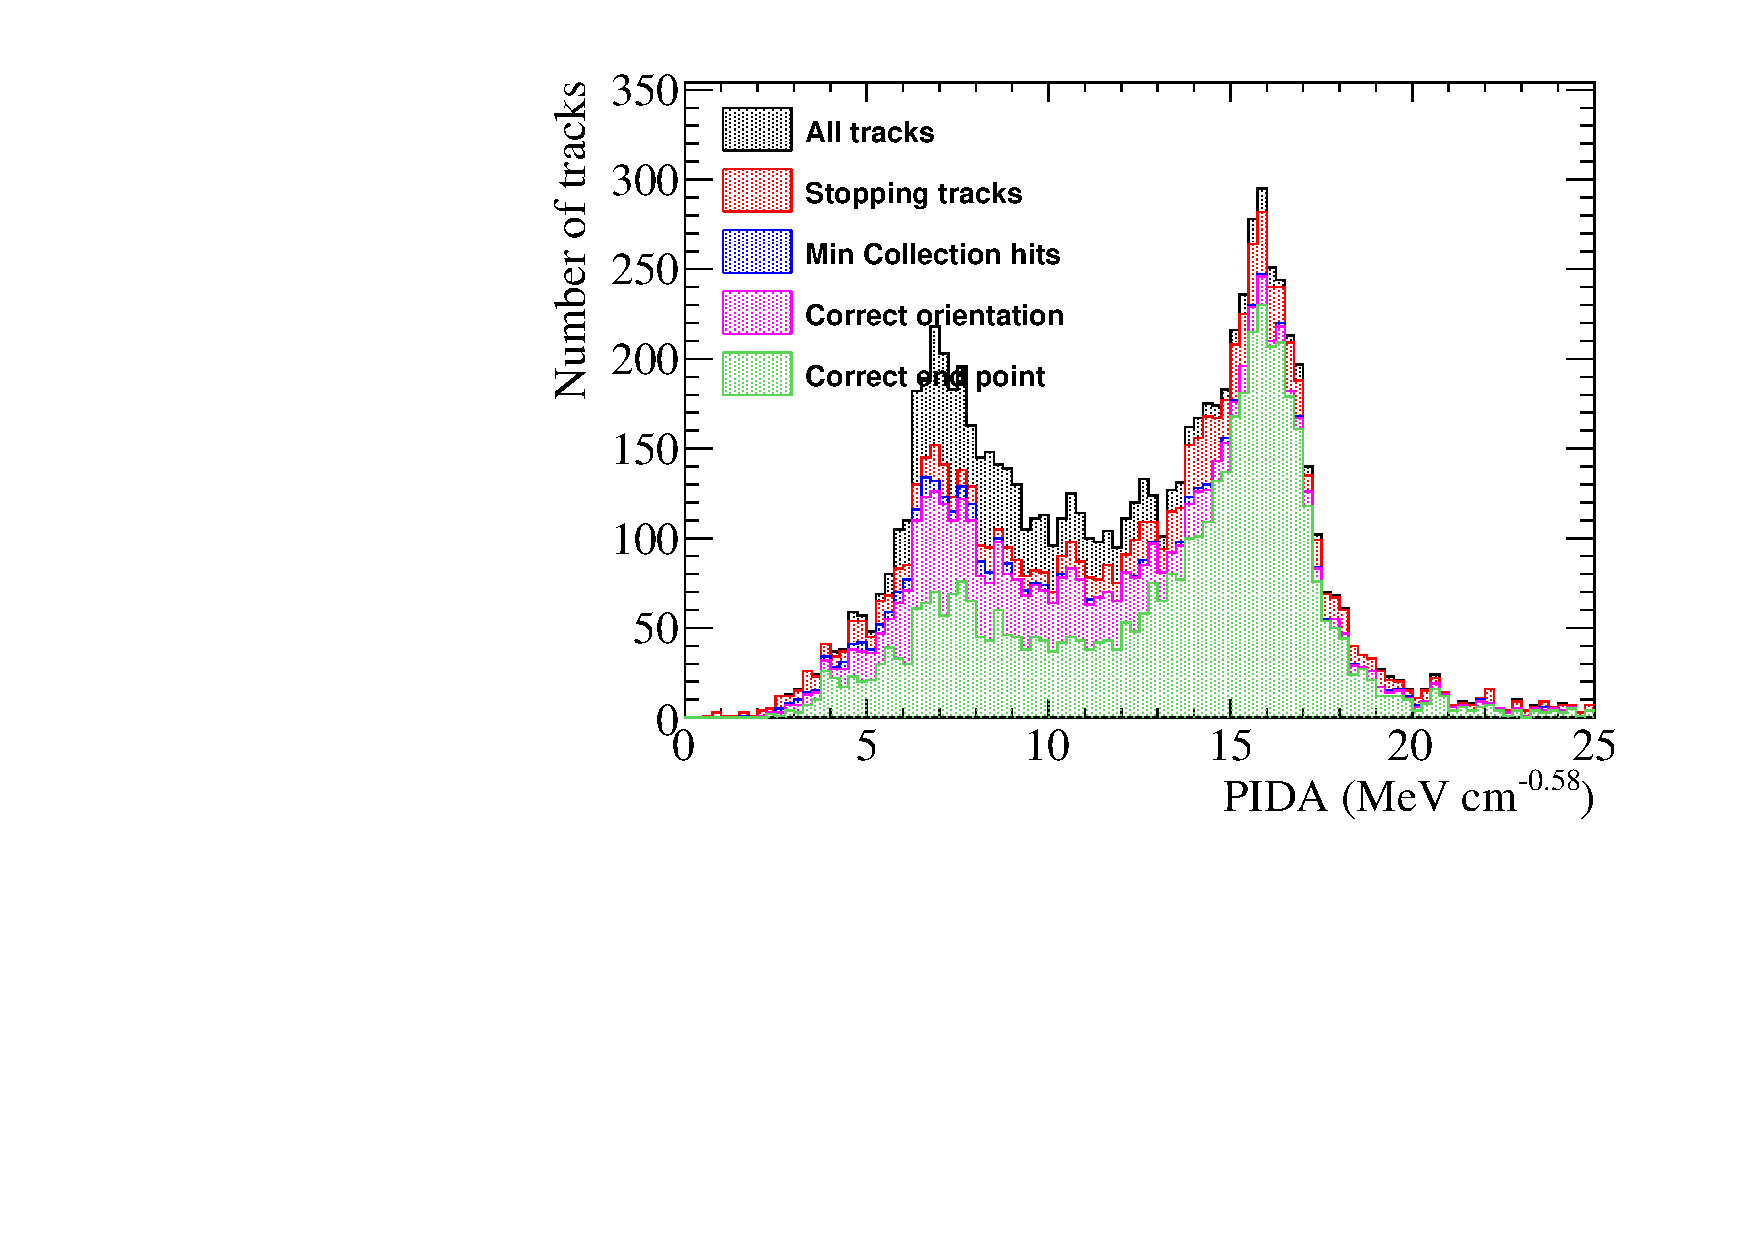
\includegraphics[width=\textwidth]{IsolatedProtons_500V_Dec16_Proton_PIDA}
        \caption{The PIDA values calculated for the single proton sample.}
        \label{fig:Isol_PIDA_Proton}
  \end{subfigure}
  \hspace{0.08\textwidth}
  \begin{subfigure}{.45\textwidth}
        \centering
        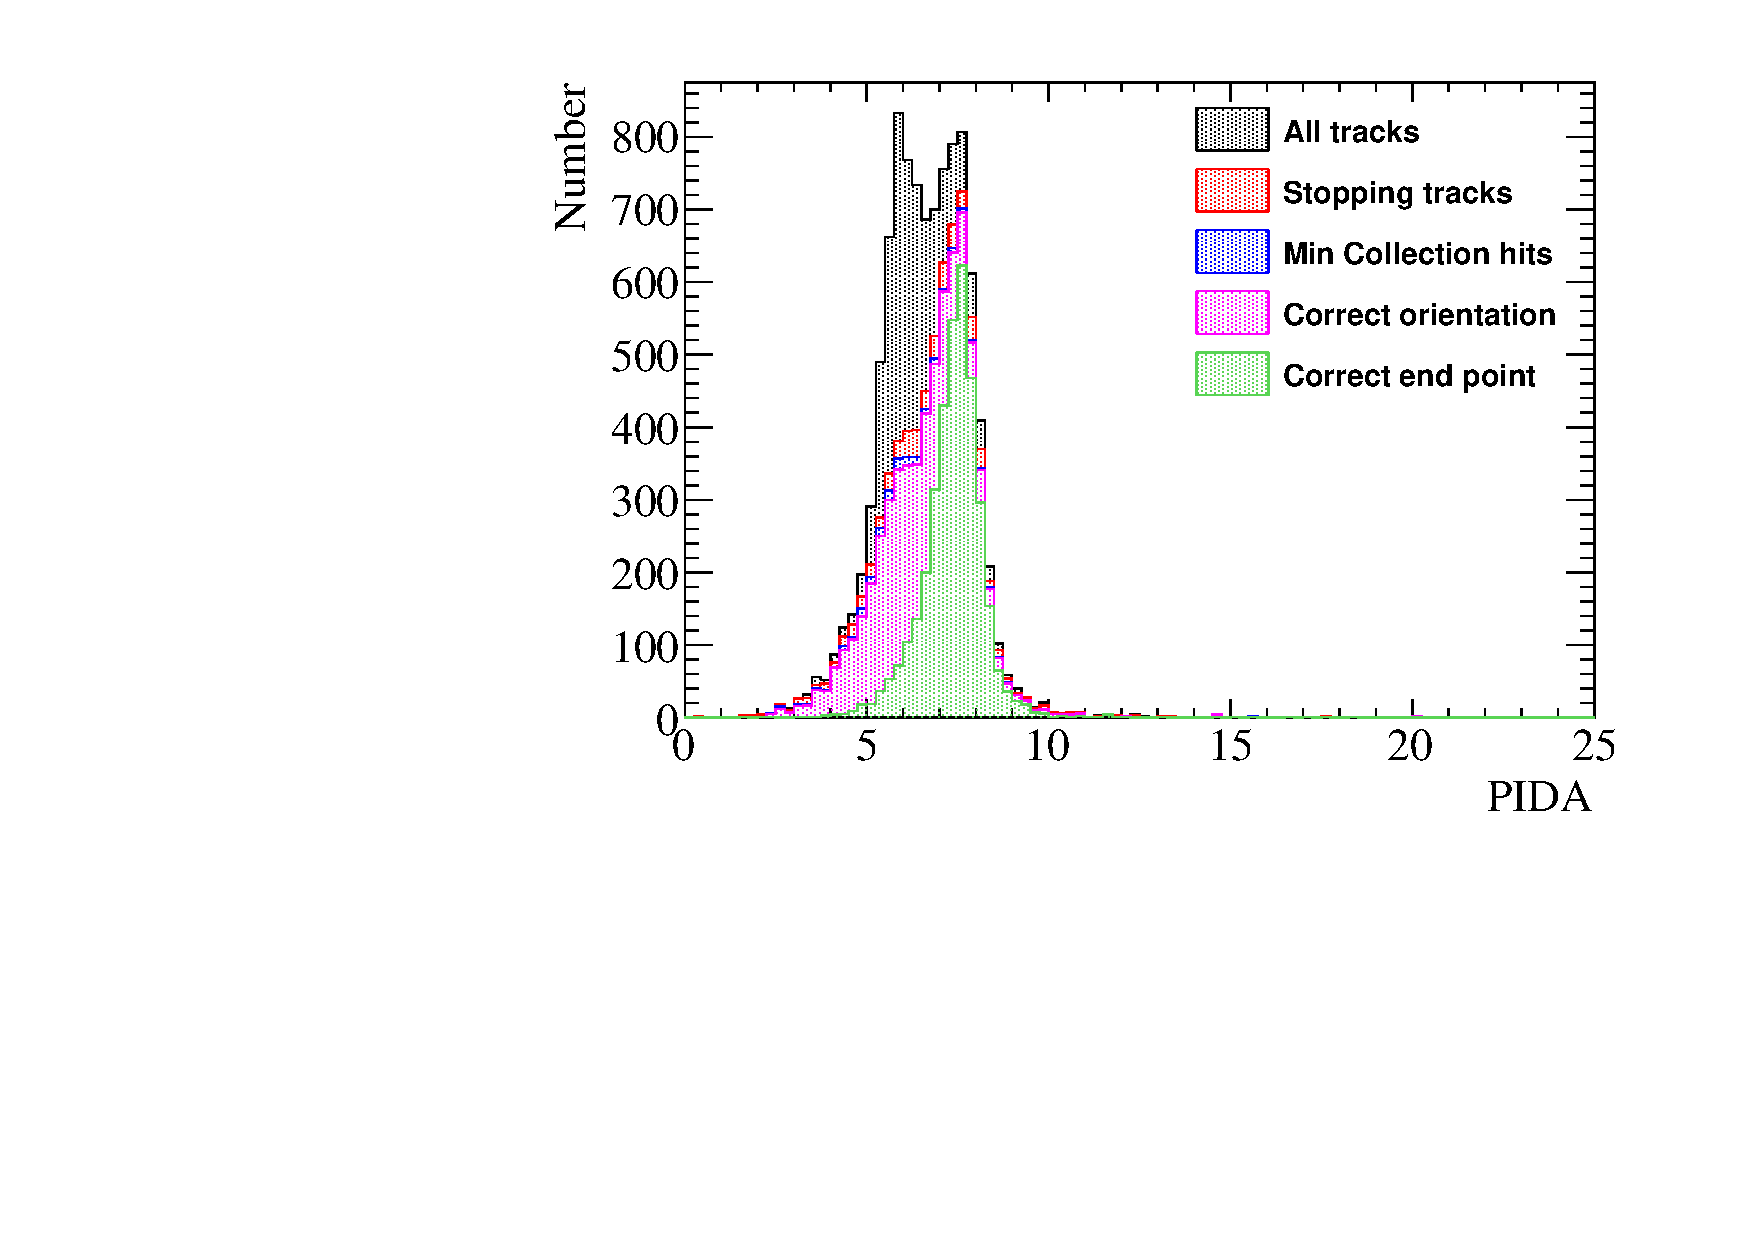
\includegraphics[width=\textwidth]{IsolatedMuons_500V_Dec16_Muon_PIDA}
        \caption{The PIDA values calculated for the single muon sample.}
        \label{fig:Isol_PIDA_Muon}
  \end{subfigure}
  \caption[The calculated PIDA values for single muons and protons in the 35 ton.]
          {The calculated PIDA values for single muons and protons in the 35 ton. A series of criteria designed to select only tracks due to stopping particles which have a required number of collection plane hits is applied. The tracks are then further refined using truth information such as the true end point of the particle.}
  \label{fig:Isol_PIDA}
\end{figure}

As can be seen from Figure~\ref{fig:Isol_PIDA} using truth information can make the distributions much cleaner, particularly when discounting particles for which the reconstruction algorithms do not track to their end point. A track is identified as having a correct end point if the reconstructed end point is within 2.5 cm of the true end point of the particle. It is reassuring to see that few tracks are reconstructed backwards, as if this were not the case then performing particle identification would be very difficult as it would indicate that the calorimetry and tracking algorithms are not performing well. Improvements can still be made though, as both plots in Figure~\ref{fig:Isol_PIDA} contain tracks which do not have the final energy depositions. This can seen as when tracks which do not match with the true end points of the particles are removed the low tails of the PIDA distributions are significantly reduced. It is observed that the PIDA distributions are cleaner when information from all three wire planes are used as opposed to only using the collection plane and so that is what is presented here. This shows how important it is to calibrate the electronics responses of all three wire planes and how additional wire planes can improve calorimetry as well as the accuracy of reconstruction algorithms. \\

The relationship between the $\frac{dE}{dx}$ and residual range of a track is shown in Figure~\ref{fig:Isol_dEdx} for both protons and muons. The much steeper increase in $\frac{dE}{dx}$ at low residual range for protons compared to muons is clearly visible when comparing Figures~\ref{fig:Isol_dEdx_Proton} and~\ref{fig:Isol_dEdx_Muon}. The contamination in the proton sample at low PIDA can be seen in Figure~\ref{fig:Isol_dEdx_Proton} where there is a clear sample of tracks for which the $\frac{dE}{dx}$ does not increase for low residual ranges. These plots are filled after tracks which do not correlate to the ends of the true trajectories are removed, and so the tail of low $\frac{dE}{dx}$ values is due to particles for which the simulated detector did not find increased energy depositions as the particle stopped. It is interesting to note that when a simple version of PIDA is calculated using the MC truth energy deposits, shown in Figure~\ref{fig:MCPIDA}, these particles are also found to have low PIDA values. It is therefore possible that at least some of these protons do not in fact stop, but interact inelastically when they still have a significant amount of kinetic energy meaning that GEANT4 will create a new particle and the tracking algorithms are creating a new track after this interaction. \\

\begin{figure}[h!]
  \centering
  \begin{subfigure}{.45\textwidth}
        \centering
        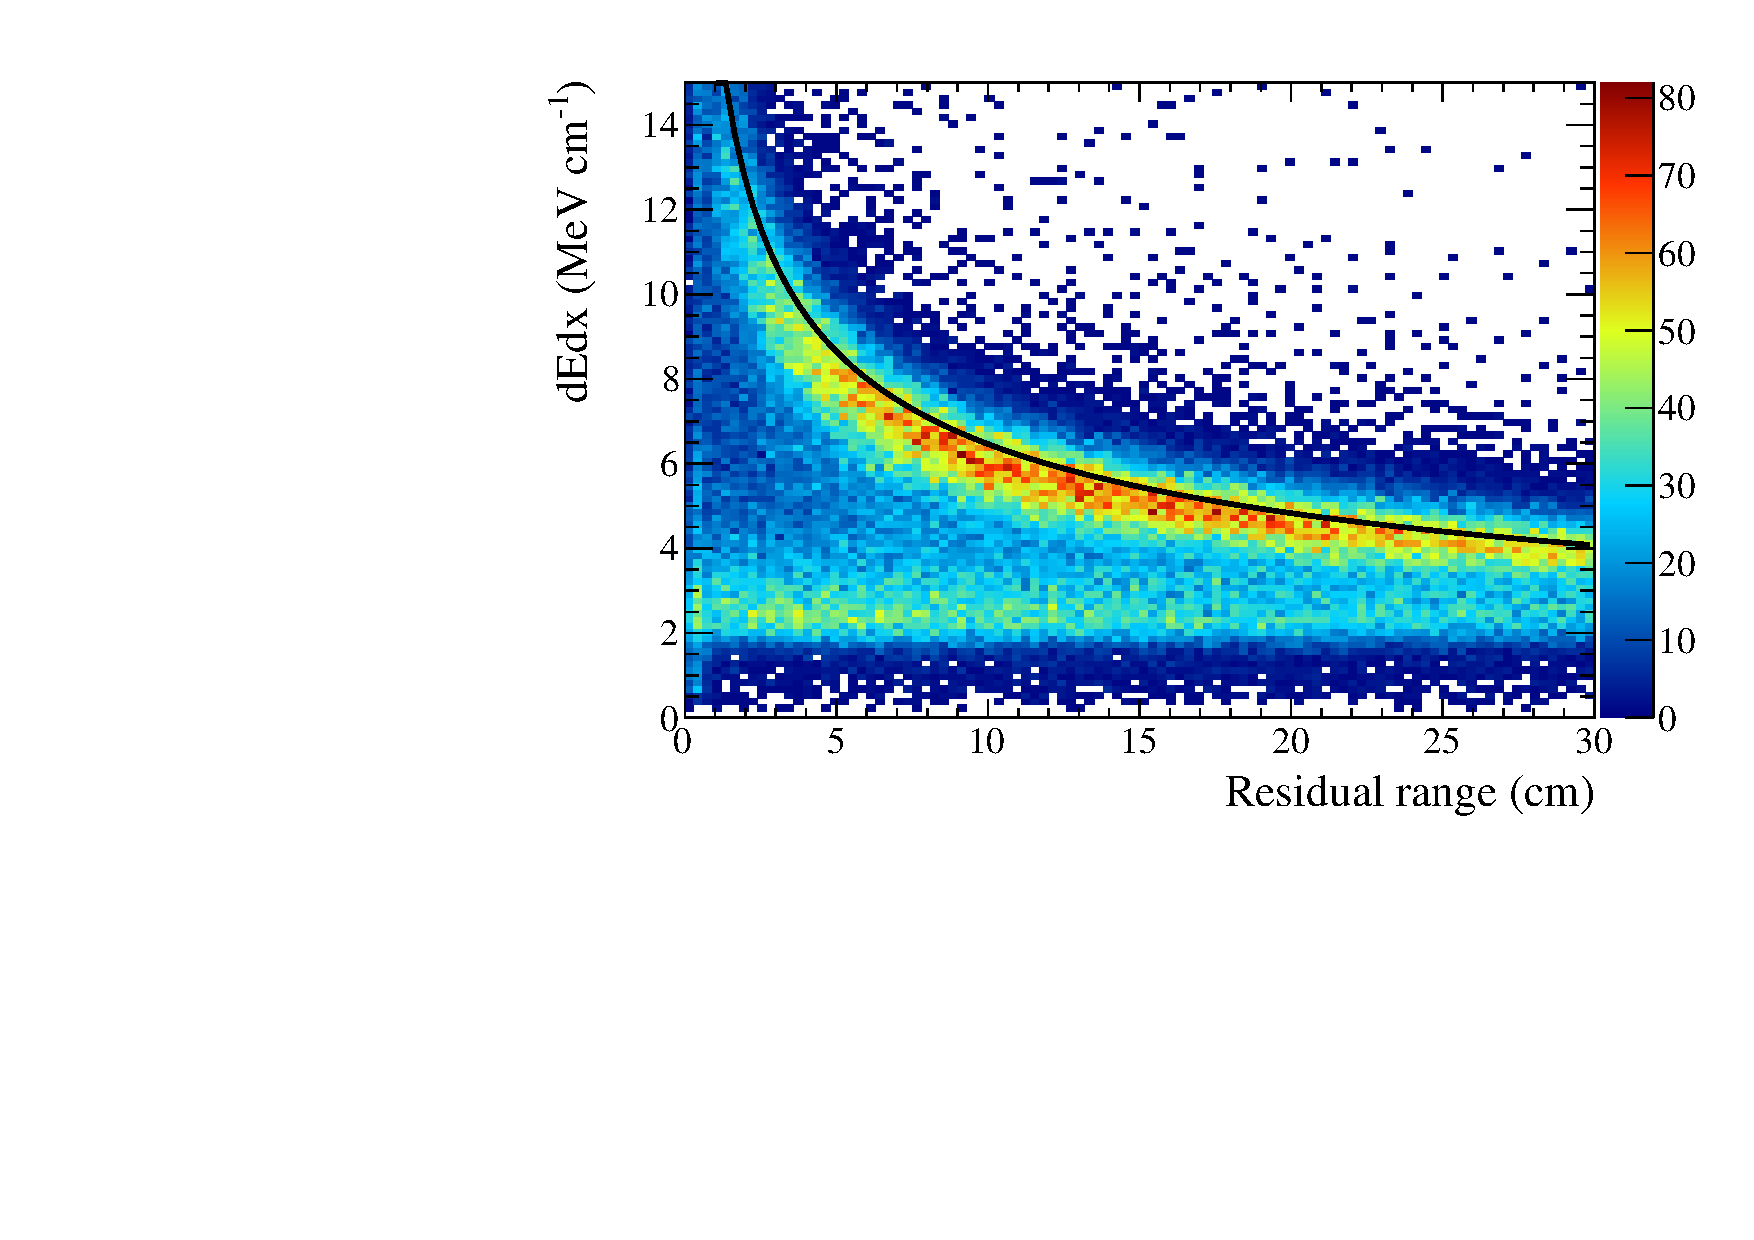
\includegraphics[width=\textwidth]{IsolatedProtons_500V_Dec16_Proton_dEdx}
        \caption{The $\frac{dE}{dx}$ versus residual range plot for the single proton sample.}
        \label{fig:Isol_dEdx_Proton}
  \end{subfigure}
  \hspace{0.08\textwidth}
  \begin{subfigure}{.45\textwidth}
        \centering
        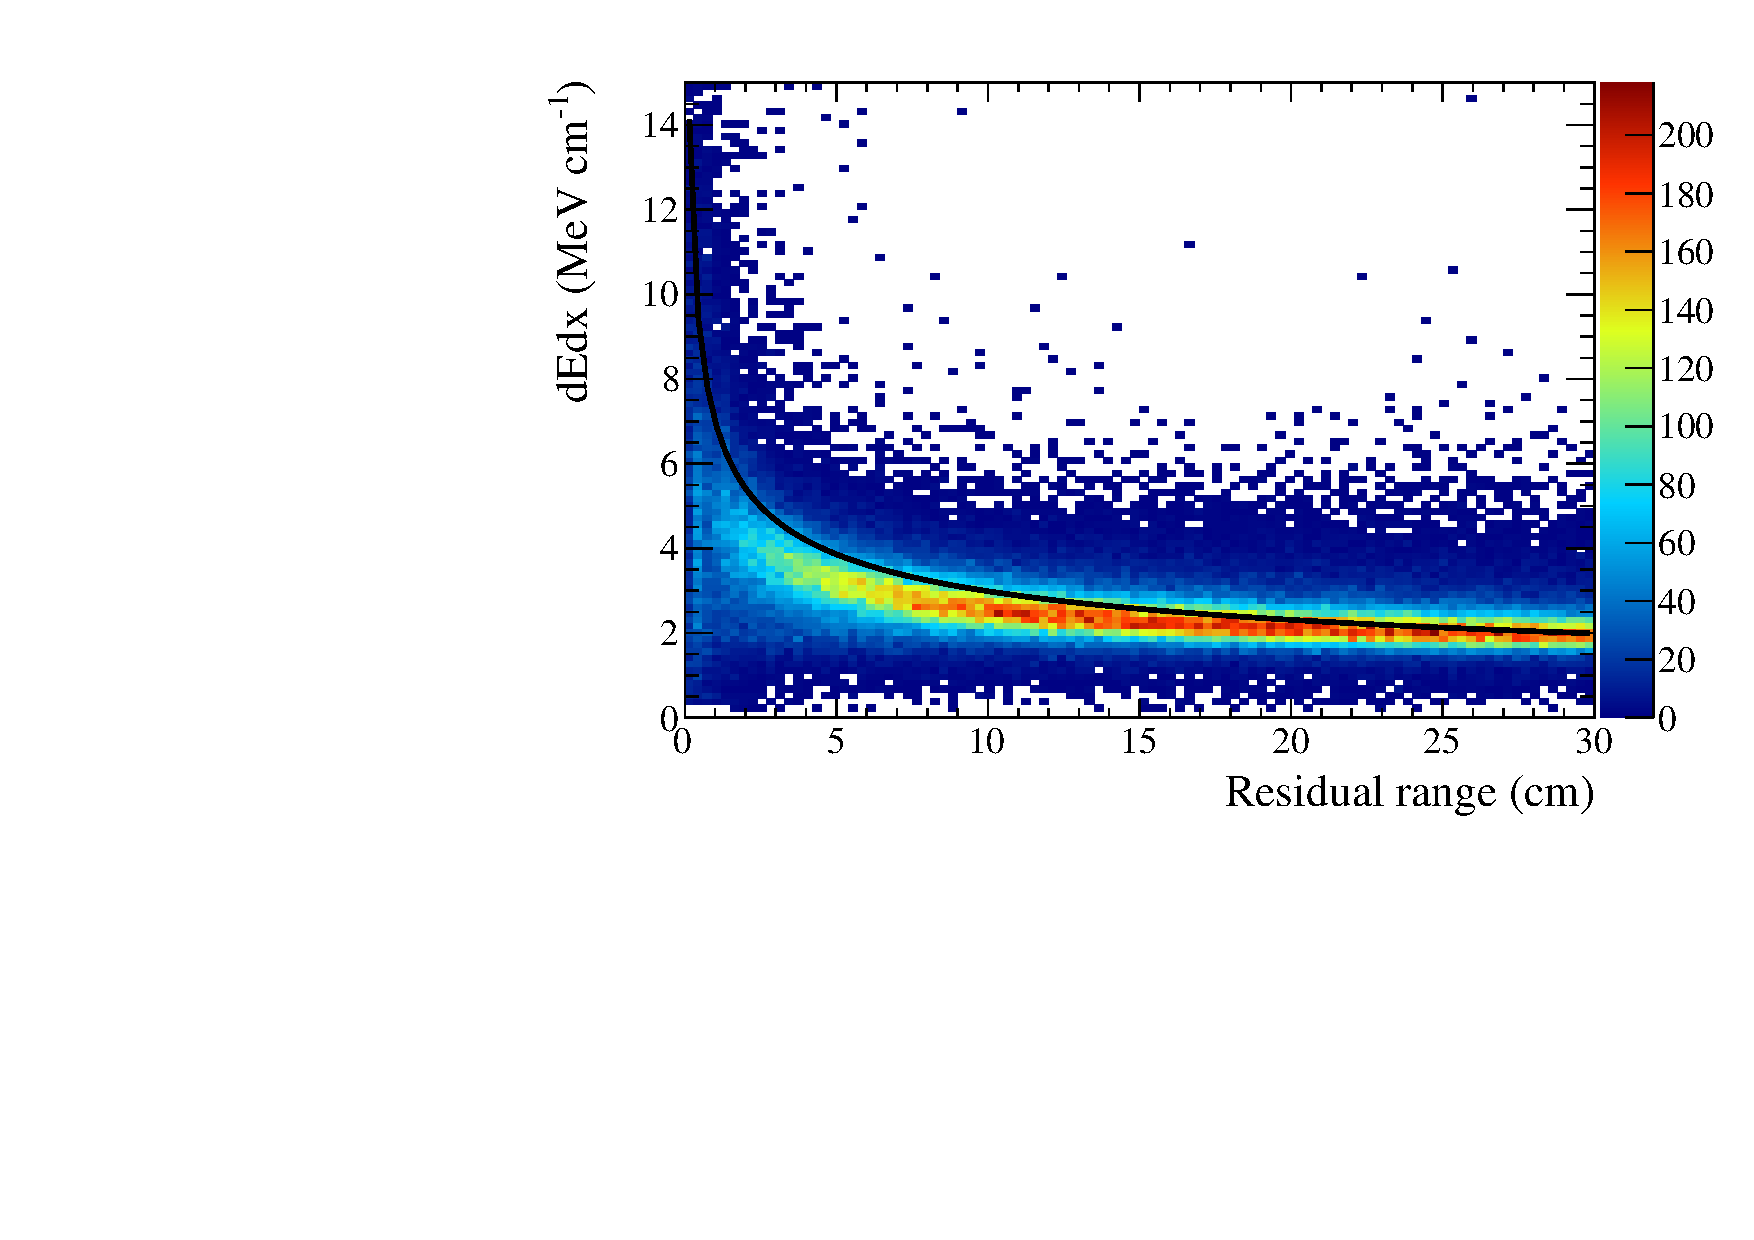
\includegraphics[width=\textwidth]{IsolatedMuons_500V_Dec16_Muon_dEdx}
        \caption{The $\frac{dE}{dx}$ versus residual range plot for the single muon sample.}
        \label{fig:Isol_dEdx_Muon}
  \end{subfigure}
  \caption[The $\frac{dE}{dx}$ versus residual range plot for single muons and protons in the 35 ton.]
          {The measured relationship between $\frac{dE}{dx}$ and residual range for single muons and protons in the 35 ton. The plots are made after applying all of the cuts outlined in Figure~\ref{fig:Isol_PIDA}, meaning that the MIP peaks have been suppressed using truth information.}
  \label{fig:Isol_dEdx}
\end{figure}

\begin{figure}[h!]
  \centering
  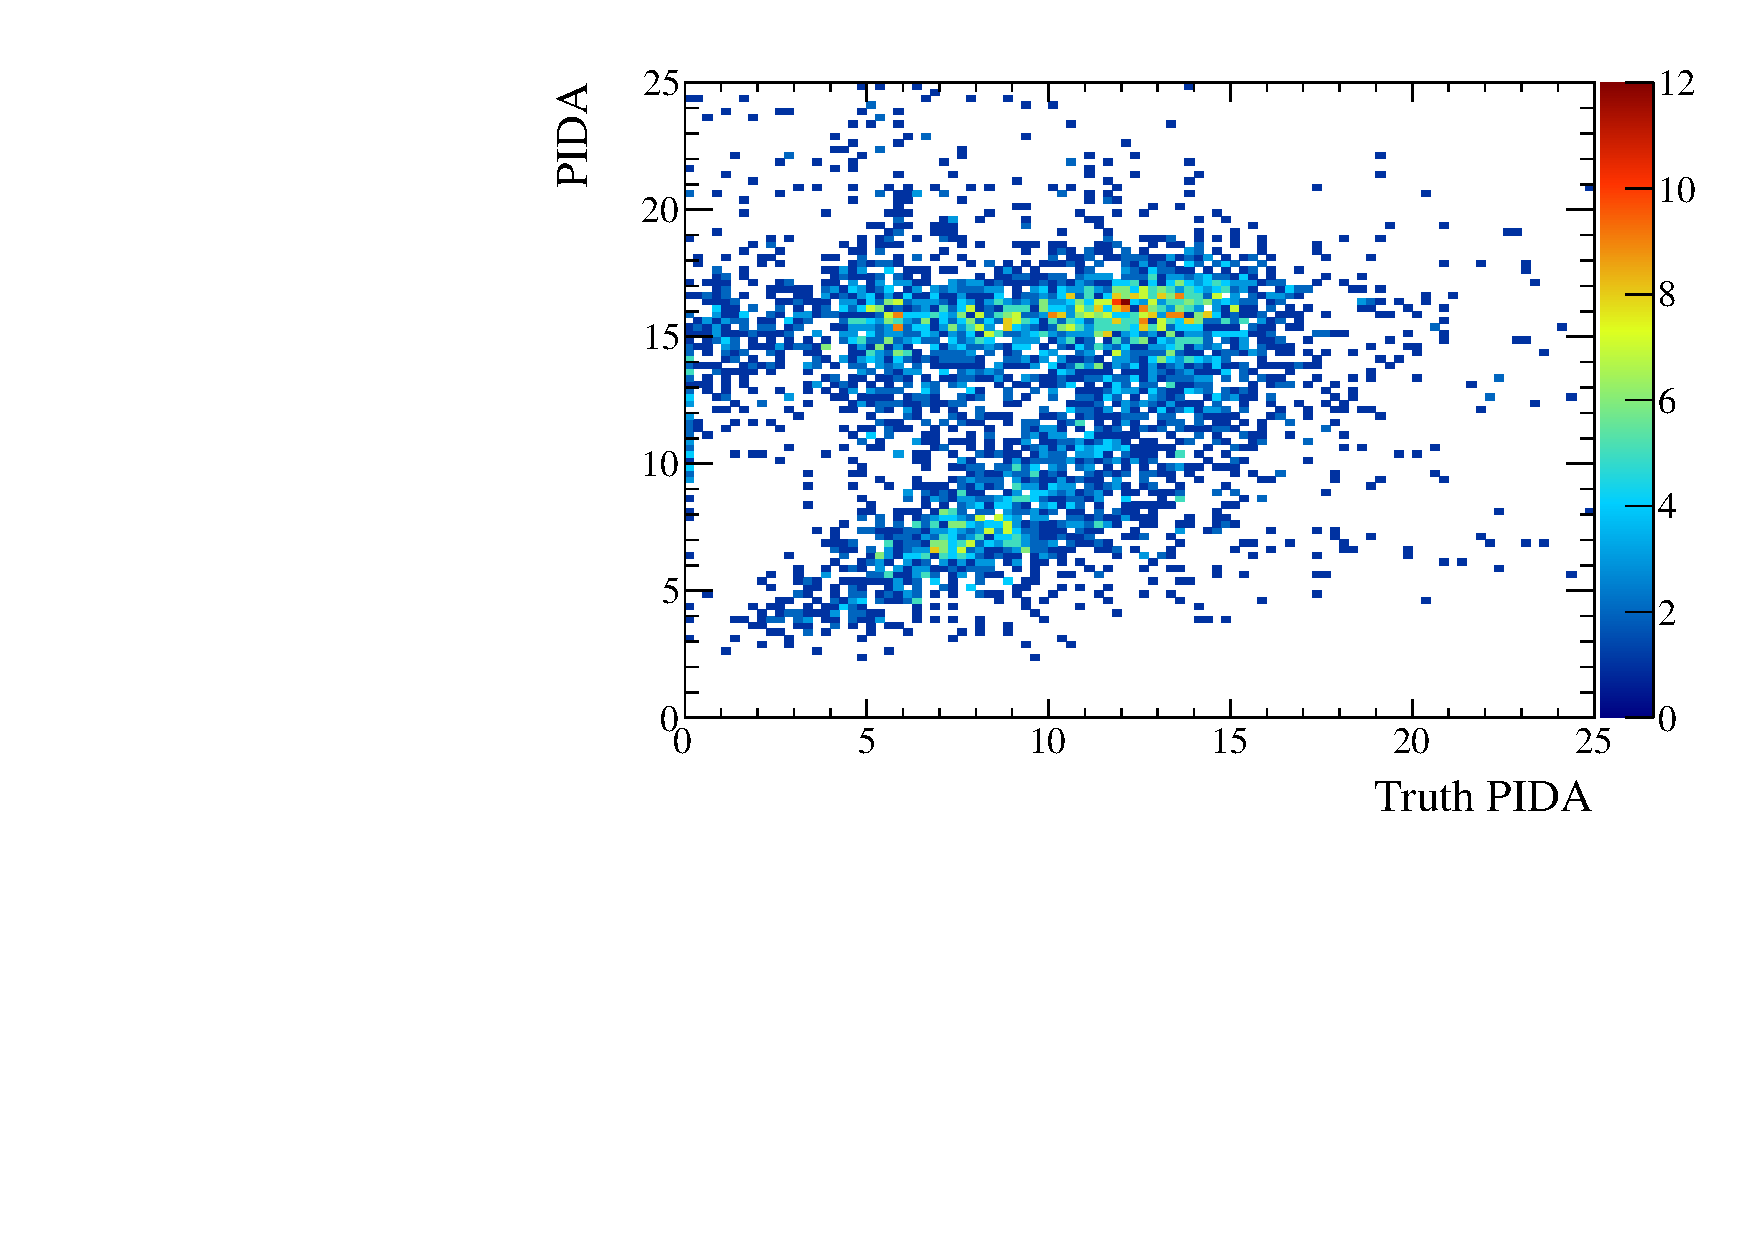
\includegraphics[width=0.5\textwidth]{IsolatedProtons_500V_Dec16_Proton_MCPIDA_PIDA}
  \caption[A comparison between PIDA values calculated using truth and reconstructed information]
          {A comparison between PIDA values calculated using truth and reconstructed information}
  \label{fig:MCPIDA}
\end{figure}

It is useful to summarise the information shown in Figure~\ref{fig:Isol_PIDA} in a table so that an efficiency of identifying stopping particles can be found. This is shown in Table~\ref{tab:Isol_PIDA_Proton} for protons, and in Table~\ref{tab:Isol_PIDA_Muon} for muons. The efficiency shown in these tables is defined as the number of tracks in the PIDA range divided by the total number of stopping particles, this is why the 'efficiency' is more than 100\% for the number of reconstructed tracks in Table~\ref{tab:Isol_PIDA_Muon}. The purity shown in these tables is defined as the percentage of tracks in the PIDA range which are associated with particles which actually stop in the detector. As many of the reconstructed tracks shown in Table~\ref{tab:Isol_PIDA_Muon} are not due to stopping particles the purity is low. The PIDA ranges referred to are 14-18 and 5-9 for the protons and muons respectively, as these ranges cover the peaks of the distributions shown in Figure~\ref{fig:Isol_dEdx} and are centered on the peaks in Figure~\ref{fig:PIDA_MC}. \\

As can be seen in Table~\ref{tab:Isol_PIDA_Proton} the efficiency upon which protons can be identified does not change significantly as the sequential criteria are applied, but as shown in Figure~\ref{fig:Isol_PIDA_Proton} the low PIDA peak decreases significantly. The same cannot be said for the muon sample however, as when the criteria that the tracking end point matches the true end point is applied a significant section of the tail within the PIDA range is removed. The resulting distribution is more similar to the distribution shown in Figure~\ref{fig:PIDA_MC} though, showing that it preserves the stopping tracks which are reconstructed best. The cut to remove tracks that do not have the correct end points reduces both sets of efficiencies, but if all the tracks were reconstructed with the correct end points then one can imagine that the number of tracks within the PIDA ranges would increase and the distributions would become more symmetrical as shown in Figure~\ref{fig:Isol_PIDA_Muon}. Both tables also exhibit high purities which shows that the fiducial cut designed to removing exiting particles is effective, with only 2 exiting protons being mis-identified in the proton sample. \\

\begin{table}
  \caption[A summary of the PIDA values calculated for the proton sample as sequential cuts are applied]
          {A summary of the PIDA values calculated for the proton sample as sequential cuts are applied.}
  \centering
  \label{tab:Isol_PIDA_Proton}
  \begin{tabular}{l c c c c}
    \toprule
    \multirow{2}{*}{Applied cut} & \multicolumn{3}{c}{Proton sample} \\ 
    \cmidrule{2-5}
      & Tracks & In PIDA range & Efficiency & Purity \\ 
    \midrule
      Total stopping particles            & 13295 &     &        & \\

      Reconstructed tracks                & 8761 & 3009 & 22.6\% & 98.7\% \\

      Survives 5 cm fiducial cut          & 7552 & 2894 & 21.8\% & 99.9\% \\

      Minimum of 10 collection plane hits & 6186 & 2507 & 18.9\% & 99.9\% \\

      Correct track orientation           & 6022 & 2491 & 18.7\% & 99.9\% \\

      Correct tracking end point          & 4432 & 2288 & 17.2\% & 100\% \\
    \bottomrule
  \end{tabular}
\end{table}

\begin{table}
  \caption[A summary of the PIDA values calculated for the proton sample as sequential cuts are applied]
          {A summary of the PIDA values calculated for the proton sample as sequential cuts are applied.}
  \centering
  \label{tab:Isol_PIDA_Muon}
  \begin{tabular}{l c c c c}
    \toprule
    \multirow{2}{*}{Applied cut} & \multicolumn{3}{c}{Muon sample} \\ 
    \cmidrule{2-5}
      & Tracks & In PIDA range & Efficiency & Purity \\ 
    \midrule
      Total stopping particles            & 6880 &      &        & \\

      Reconstructed tracks                & 9883 & 8907 & 129\%  & 67.4\% \\

      Survives 5 cm fiducial cut          & 7126 & 6259 & 90.9\% & 90.2\% \\

      Minimum of 10 collection plane hits & 6580 & 5876 & 85.4\% & 89.9\% \\

      Correct track orientation           & 6436 & 5767 & 83.8\% & 90.1\% \\

      Correct tracking end point          & 3676 & 3555 & 51.7\% & 100\%  \\
    \bottomrule
  \end{tabular}
\end{table}

From Table~\ref{tab:Isol_PIDA_Proton} it can be seen that there are more stopping protons than primary protons as only 10,000 primary protons were generated. The effectiveness of the PIDA algorithm at identifying only primary protons is shown in Table~\ref{tab:Isol_PIDA_PrimProton}. Comparing both tables it can be seen that the efficiency with which the primary protons can be identified is larger than the secondary protons as the efficiencies shown in Table~\ref{tab:Isol_PIDA_Proton} are lower than those in Table~\ref{tab:Isol_PIDA_PrimProton}. It is thought that this is due to the low reconstruction efficiency for the very shortest tracks which many of the secondary protons have, as discussed in Section~\ref{sec:SimRecoEffic}. A similar table is not produced for primary muons as there were no secondary muons produced in the muon sample, and so Table~\ref{tab:Isol_PIDA_Muon} is itself the efficiency with which the primary muons can be identified. \\ 

\begin{table}
  \caption[A summary of the PIDA values calculated for the primary particles in the proton sample as sequential cuts are applied]
          {A summary of the PIDA values calculated for the primary particles in the proton sample as sequential cuts are applied.}
  \centering
  \label{tab:Isol_PIDA_PrimProton}
  \begin{tabular}{l c c c c}
    \toprule
    \multirow{2}{*}{Applied cut} & \multicolumn{3}{c}{Proton sample} \\ 
    \cmidrule{2-5}
      & Tracks & In PIDA range & Efficiency & Purity \\ 
    \midrule
      Total stopping particles            & 7798 &      &        & \\

      Reconstructed tracks                & 5920 & 1937 & 24.8\% & 98.9\% \\

      Survives 5 cm fiducial cut          & 5044 & 1878 & 24.1\% & 99.9\% \\

      Minimum of 10 collection plane hits & 4485 & 1711 & 21.9\% & 99.9\% \\

      Correct track orientation           & 4363 & 1707 & 21.9\% & 99.9\% \\

      Correct tracking end point          & 3122 & 1565 & 20.1\% & 100\%  \\
    \bottomrule
  \end{tabular}
\end{table}

Upon verifying that the PIDA metric can reliably determine particle type when they are simulated in isolation, the next step is to observe the accuracy upon which particles can be identified in a CRY sample. The sample used here differs from the CRY sample used earlier in that only events which contain a proton in the detector are reconstructed, this is done to reduce simulation time and storage space as this cut will still provide a substantial number of muons whilst ensuring that a large proton sample can be reconstructed. The process of calculating PIDA values for the tracks is identical in all samples, though as discussed in Section~\ref{sec:SimRecoEffic} the much more complicated event structure in the CRY sample affects the reconstruction efficiency and so will likely also affect the accuracy of the calorimetry. The calorimetry will be affected in two ways, firstly the reduced performance of the reconstruction algorithms will mean that some particles are not reconstructed at all, whilst those that are reconstructed may be more likely to have missing hits meaning that the end points may be less well reconstructed. This will cause the tail of low $\frac{dE}{dx}$ values seen in Figure~\ref{fig:Isol_dEdx_Proton} to be more pronounced. Secondly, as shown in Figure~\ref{fig:PD_MCPDDiff} though the photon detector time determination is very accurate for a large number of tracks it is also incorrect for a number of tracks, this will cause the recombination correction to be miscalculated which will in turn increase the calculated $\frac{dE}{dx}$ and hence PIDA values. \\

The PIDA values calculated for protons and muons in the CRY sample are shown in Figure~\ref{fig:CRY_PIDA}. As can be seen from Figure~\ref{fig:CRY_PIDA_Muon} there is a tail of very high PIDA value muon tracks which contaminate the proton PIDA region of interest (ROI). This causes a serious problem when trying to identify protons from a cosmic sample as the number of muons present is significantly larger than the number of protons. The result of this will be a sample of tracks which will not be very pure, and so further cuts will have to be developed to enhance the purity of this sample whilst not reducing the efficiency upon which proton tracks are identified. \\

\begin{figure}[h!]
  \centering
  \begin{subfigure}{.45\textwidth}
        \centering
        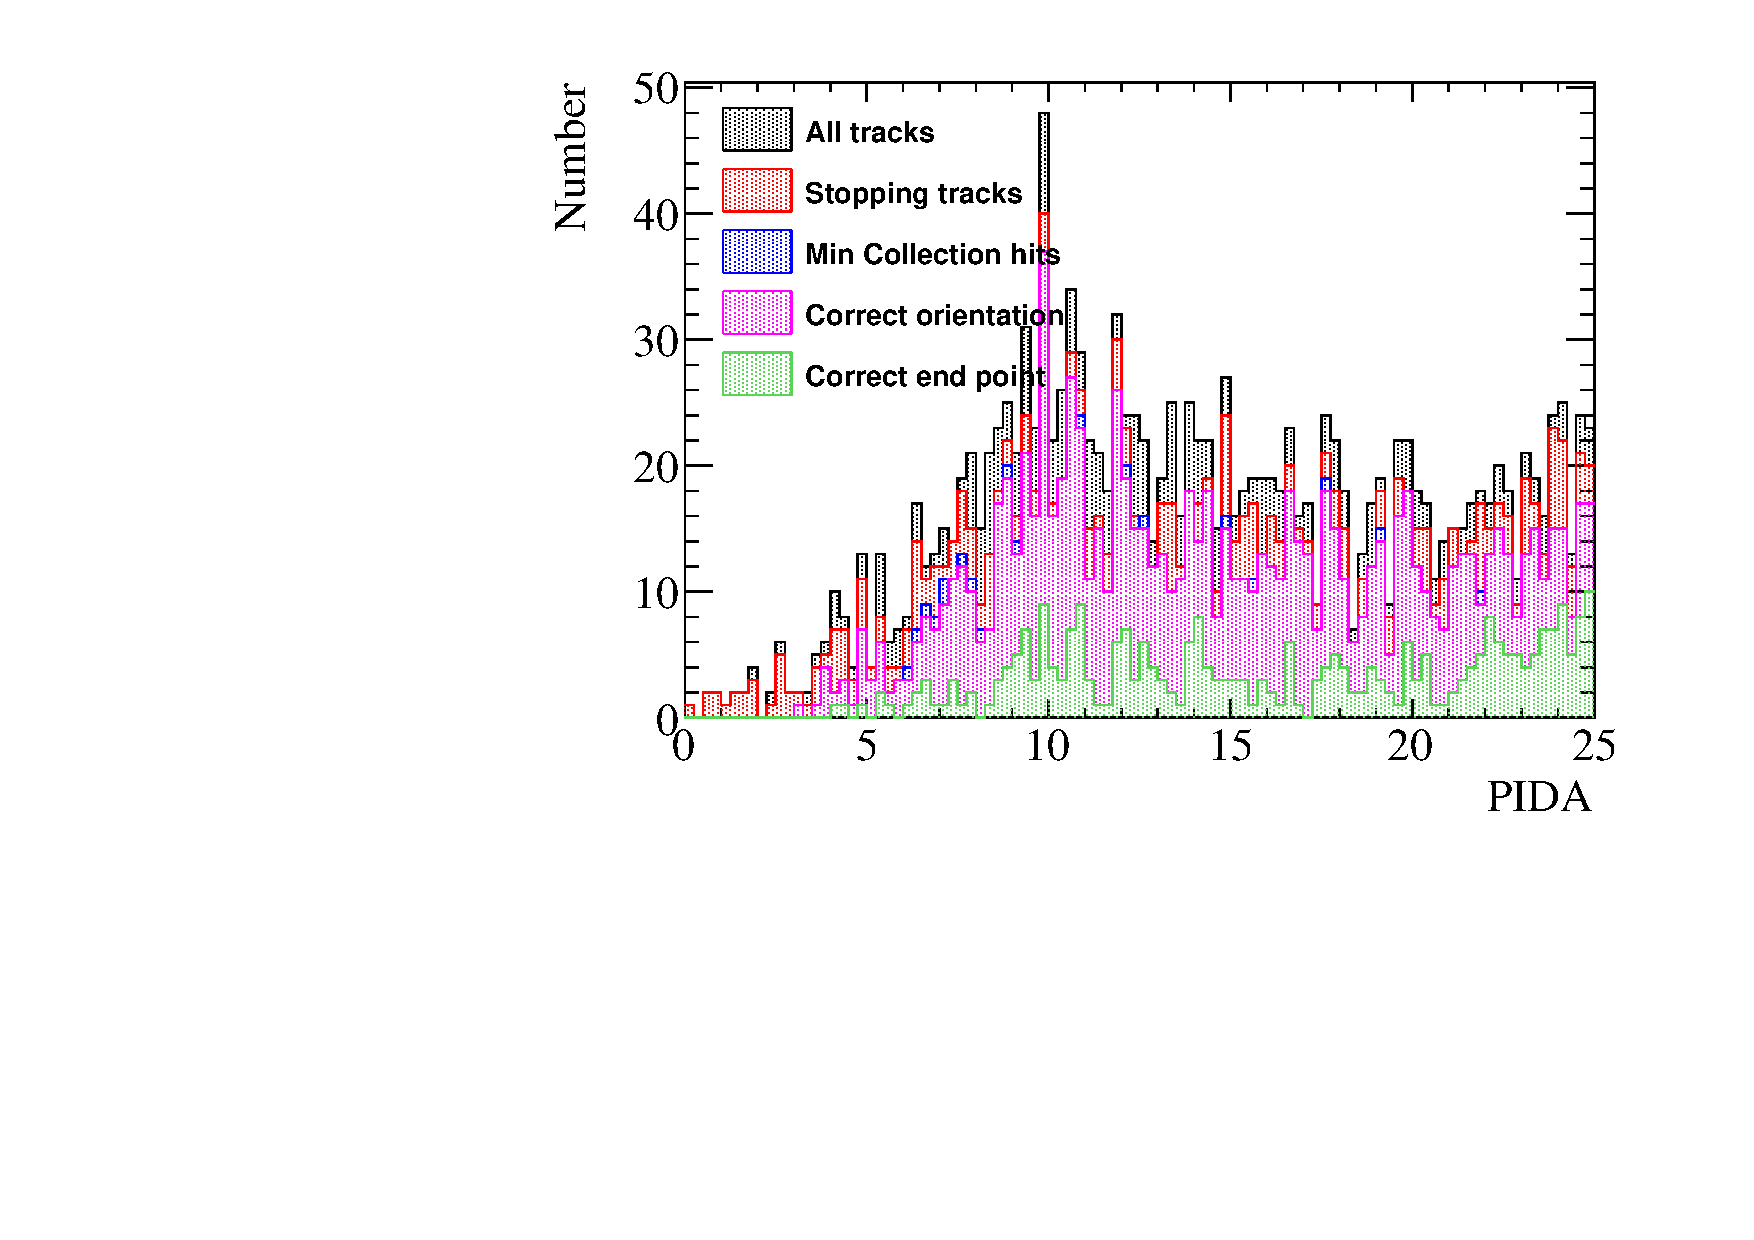
\includegraphics[width=\textwidth]{EnrinchedSample_500V_v06_18_00_Proton_PIDA}
        \caption{The PIDA values calculated for protons.}
        \label{fig:CRY_PIDA_Proton}
  \end{subfigure}
  \hspace{0.08\textwidth}
  \begin{subfigure}{.45\textwidth}
        \centering
        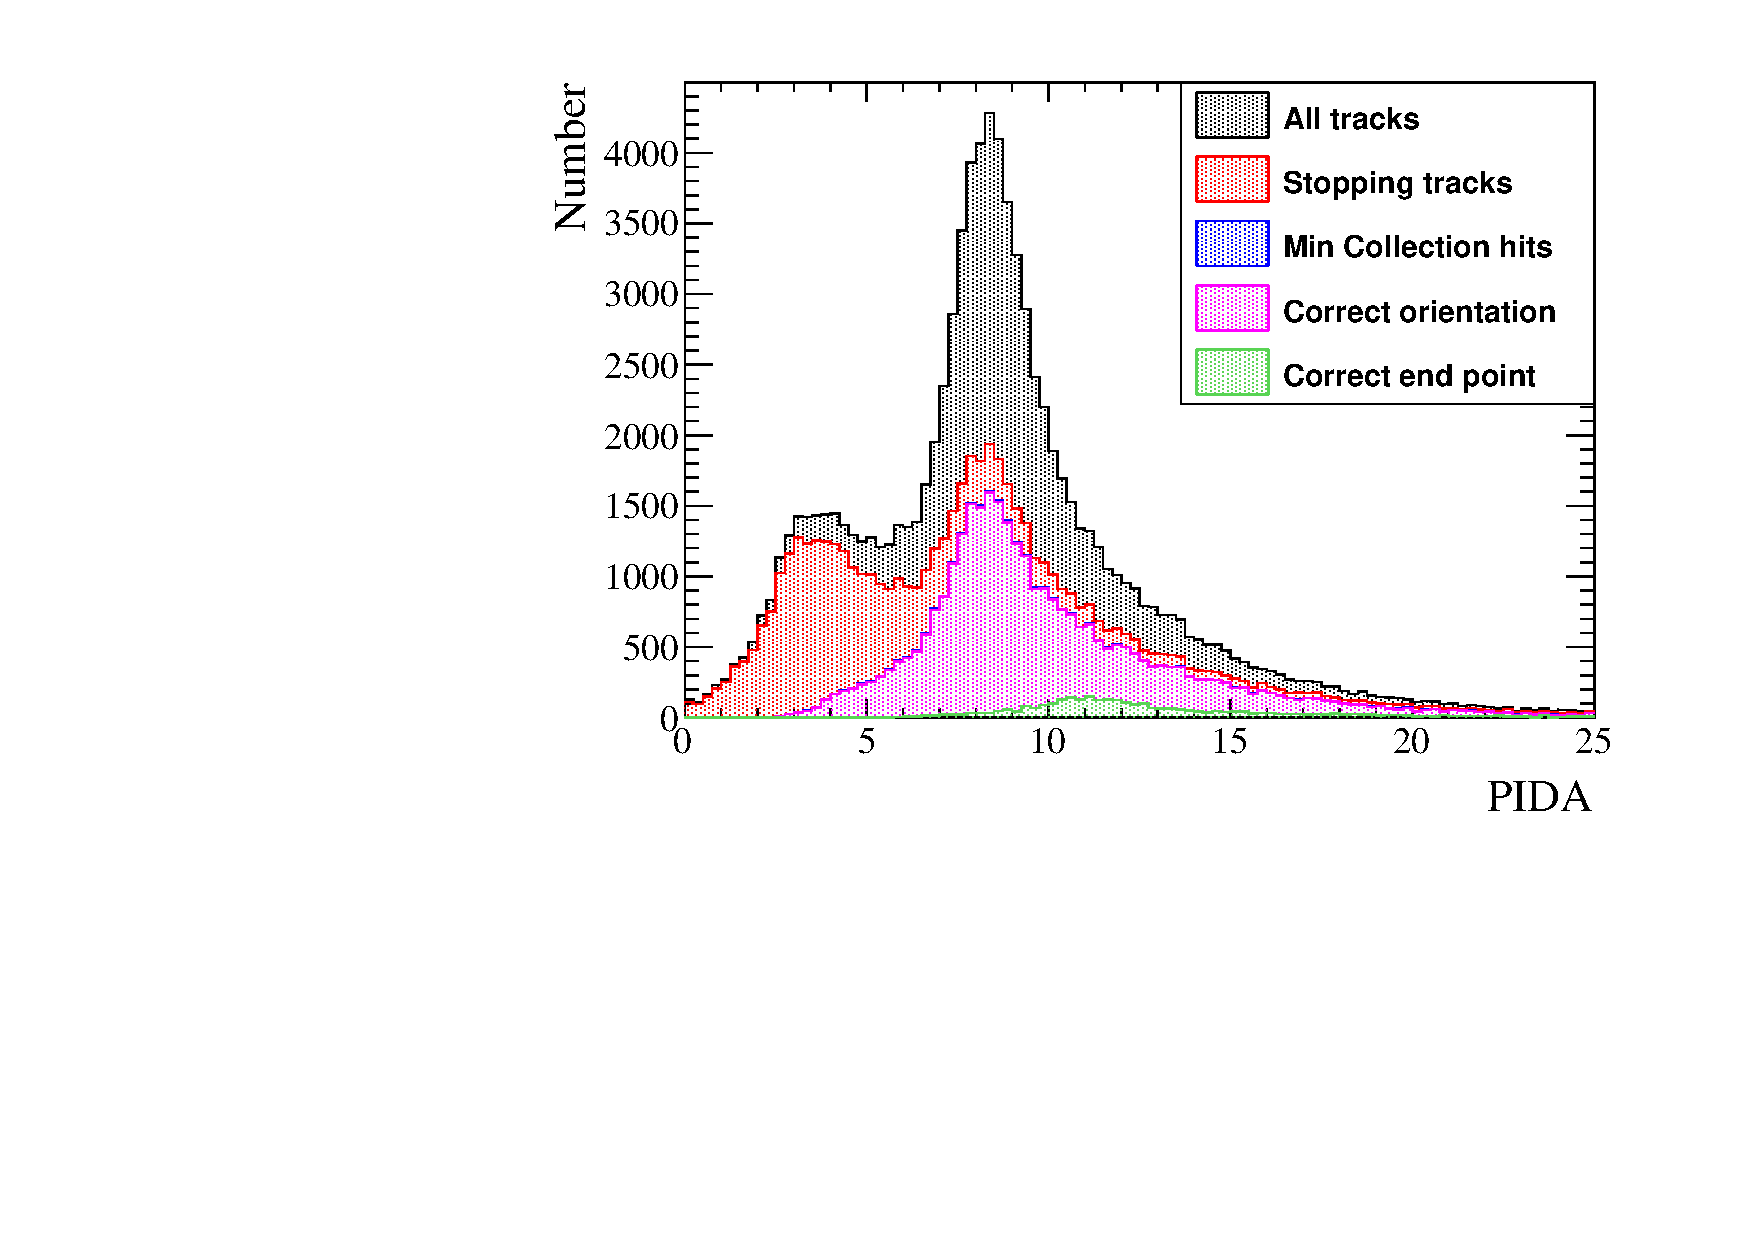
\includegraphics[width=\textwidth]{EnrinchedSample_500V_v06_18_00_Muon_PIDA}
        \caption{The PIDA values calculated for muons.}
        \label{fig:CRY_PIDA_Muon}
  \end{subfigure}
  \caption[The calculated PIDA values for muons and protons in a CRY sample through the 35 ton]
          {The calculated PIDA values for muons and protons in a CRY sample through the 35 ton. A series of criteria designed to select only tracks due to stopping particles which have a required number of collection plane hits is applied. The tracks are then further refined using truth information such as the true end point of the particle.}
  \label{fig:CRY_PIDA}
\end{figure}
